% Options for packages loaded elsewhere
\PassOptionsToPackage{unicode}{hyperref}
\PassOptionsToPackage{hyphens}{url}
\PassOptionsToPackage{dvipsnames,svgnames*,x11names*}{xcolor}
%
\documentclass[
  russian,
]{article}
\usepackage{amsmath,amssymb}
\usepackage{lmodern}
\usepackage{iftex}
\ifPDFTeX
  \usepackage[T1]{fontenc}
  \usepackage[utf8]{inputenc}
  %
  %\usepackage{polyglossia}
  %\usepackage[utf8x]{inputenc}
  %\usepackage[english,russian]{babel}
  %\setmainlanguage{russian}
  %
  \usepackage{textcomp} % provide euro and other symbols
\else % if luatex or xetex
  \usepackage{unicode-math}
  \defaultfontfeatures{Scale=MatchLowercase}
  \defaultfontfeatures[\rmfamily]{Ligatures=TeX,Scale=1}
\fi
% Use upquote if available, for straight quotes in verbatim environments
\IfFileExists{upquote.sty}{\usepackage{upquote}}{}
\IfFileExists{microtype.sty}{% use microtype if available
  \usepackage[]{microtype}
  \UseMicrotypeSet[protrusion]{basicmath} % disable protrusion for tt fonts
}{}
\makeatletter
\@ifundefined{KOMAClassName}{% if non-KOMA class
  \IfFileExists{parskip.sty}{%
    \usepackage{parskip}
  }{% else
    \setlength{\parindent}{0pt}
    \setlength{\parskip}{6pt plus 2pt minus 1pt}}
}{% if KOMA class
  \KOMAoptions{parskip=half}}
\makeatother
\usepackage{xcolor}
\IfFileExists{xurl.sty}{\usepackage{xurl}}{} % add URL line breaks if available
\IfFileExists{bookmark.sty}{\usepackage{bookmark}}{\usepackage{hyperref}}
\hypersetup{
  pdftitle={Начало работы},
  pdflang={ru-RU},
  colorlinks=true,
  linkcolor={blue},
  filecolor={Maroon},
  citecolor={Blue},
  urlcolor={Blue},
  pdfcreator={LaTeX via pandoc}}
\urlstyle{same} % disable monospaced font for URLs
\usepackage{color}
\usepackage{fancyvrb}
\newcommand{\VerbBar}{|}
\newcommand{\VERB}{\Verb[commandchars=\\\{\}]}
\DefineVerbatimEnvironment{Highlighting}{Verbatim}{commandchars=\\\{\}}
% Add ',fontsize=\small' for more characters per line
\usepackage{framed}
\definecolor{shadecolor}{RGB}{241,243,245}
\newenvironment{Shaded}{\begin{snugshade}}{\end{snugshade}}
\newcommand{\AlertTok}[1]{\textcolor[rgb]{0.68,0.00,0.00}{#1}}
\newcommand{\AnnotationTok}[1]{\textcolor[rgb]{0.37,0.37,0.37}{#1}}
\newcommand{\AttributeTok}[1]{\textcolor[rgb]{0.40,0.45,0.13}{#1}}
\newcommand{\BaseNTok}[1]{\textcolor[rgb]{0.68,0.00,0.00}{#1}}
\newcommand{\BuiltInTok}[1]{\textcolor[rgb]{0.00,0.23,0.31}{#1}}
\newcommand{\CharTok}[1]{\textcolor[rgb]{0.13,0.47,0.30}{#1}}
\newcommand{\CommentTok}[1]{\textcolor[rgb]{0.37,0.37,0.37}{#1}}
\newcommand{\CommentVarTok}[1]{\textcolor[rgb]{0.37,0.37,0.37}{\textit{#1}}}
\newcommand{\ConstantTok}[1]{\textcolor[rgb]{0.56,0.35,0.01}{#1}}
\newcommand{\ControlFlowTok}[1]{\textcolor[rgb]{0.00,0.23,0.31}{\textbf{#1}}}
\newcommand{\DataTypeTok}[1]{\textcolor[rgb]{0.68,0.00,0.00}{#1}}
\newcommand{\DecValTok}[1]{\textcolor[rgb]{0.68,0.00,0.00}{#1}}
\newcommand{\DocumentationTok}[1]{\textcolor[rgb]{0.37,0.37,0.37}{\textit{#1}}}
\newcommand{\ErrorTok}[1]{\textcolor[rgb]{0.68,0.00,0.00}{#1}}
\newcommand{\ExtensionTok}[1]{\textcolor[rgb]{0.00,0.23,0.31}{#1}}
\newcommand{\FloatTok}[1]{\textcolor[rgb]{0.68,0.00,0.00}{#1}}
\newcommand{\FunctionTok}[1]{\textcolor[rgb]{0.28,0.35,0.67}{#1}}
\newcommand{\ImportTok}[1]{\textcolor[rgb]{0.00,0.46,0.62}{#1}}
\newcommand{\InformationTok}[1]{\textcolor[rgb]{0.37,0.37,0.37}{#1}}
\newcommand{\KeywordTok}[1]{\textcolor[rgb]{0.00,0.23,0.31}{\textbf{#1}}}
\newcommand{\NormalTok}[1]{\textcolor[rgb]{0.00,0.23,0.31}{#1}}
\newcommand{\OperatorTok}[1]{\textcolor[rgb]{0.37,0.37,0.37}{#1}}
\newcommand{\OtherTok}[1]{\textcolor[rgb]{0.00,0.23,0.31}{#1}}
\newcommand{\PreprocessorTok}[1]{\textcolor[rgb]{0.68,0.00,0.00}{#1}}
\newcommand{\RegionMarkerTok}[1]{\textcolor[rgb]{0.00,0.23,0.31}{#1}}
\newcommand{\SpecialCharTok}[1]{\textcolor[rgb]{0.37,0.37,0.37}{#1}}
\newcommand{\SpecialStringTok}[1]{\textcolor[rgb]{0.13,0.47,0.30}{#1}}
\newcommand{\StringTok}[1]{\textcolor[rgb]{0.13,0.47,0.30}{#1}}
\newcommand{\VariableTok}[1]{\textcolor[rgb]{0.07,0.07,0.07}{#1}}
\newcommand{\VerbatimStringTok}[1]{\textcolor[rgb]{0.13,0.47,0.30}{#1}}
\newcommand{\WarningTok}[1]{\textcolor[rgb]{0.37,0.37,0.37}{\textit{#1}}}
\usepackage{longtable,booktabs,array}
\usepackage{calc} % for calculating minipage widths
% Correct order of tables after \paragraph or \subparagraph
\usepackage{etoolbox}
\makeatletter
\patchcmd\longtable{\par}{\if@noskipsec\mbox{}\fi\par}{}{}
\makeatother
% Allow footnotes in longtable head/foot
\IfFileExists{footnotehyper.sty}{\usepackage{footnotehyper}}{\usepackage{footnote}}
\makesavenoteenv{longtable}
\usepackage{graphicx}
\makeatletter
\def\maxwidth{\ifdim\Gin@nat@width>\linewidth\linewidth\else\Gin@nat@width\fi}
\def\maxheight{\ifdim\Gin@nat@height>\textheight\textheight\else\Gin@nat@height\fi}
\makeatother
% Scale images if necessary, so that they will not overflow the page
% margins by default, and it is still possible to overwrite the defaults
% using explicit options in \includegraphics[width, height, ...]{}
\setkeys{Gin}{width=\maxwidth,height=\maxheight,keepaspectratio}
% Set default figure placement to htbp
\makeatletter
\def\fps@figure{htbp}
\makeatother
\setlength{\emergencystretch}{3em} % prevent overfull lines
\providecommand{\tightlist}{%
  \setlength{\itemsep}{0pt}\setlength{\parskip}{0pt}}
\setcounter{secnumdepth}{-\maxdimen} % remove section numbering
% Make \paragraph and \subparagraph free-standing
\ifx\paragraph\undefined\else
  \let\oldparagraph\paragraph
  \renewcommand{\paragraph}[1]{\oldparagraph{#1}\mbox{}}
\fi
\ifx\subparagraph\undefined\else
  \let\oldsubparagraph\subparagraph
  \renewcommand{\subparagraph}[1]{\oldsubparagraph{#1}\mbox{}}
\fi
\makeatletter
\@ifpackageloaded{tcolorbox}{}{\usepackage[skins,breakable]{tcolorbox}}
\@ifpackageloaded{fontawesome5}{}{\usepackage{fontawesome5}}
\definecolor{quarto-callout-color}{HTML}{909090}
\definecolor{quarto-callout-note-color}{HTML}{0758E5}
\definecolor{quarto-callout-important-color}{HTML}{CC1914}
\definecolor{quarto-callout-warning-color}{HTML}{EB9113}
\definecolor{quarto-callout-tip-color}{HTML}{00A047}
\definecolor{quarto-callout-caution-color}{HTML}{FC5300}
\definecolor{quarto-callout-color-frame}{HTML}{acacac}
\definecolor{quarto-callout-note-color-frame}{HTML}{4582ec}
\definecolor{quarto-callout-important-color-frame}{HTML}{d9534f}
\definecolor{quarto-callout-warning-color-frame}{HTML}{f0ad4e}
\definecolor{quarto-callout-tip-color-frame}{HTML}{02b875}
\definecolor{quarto-callout-caution-color-frame}{HTML}{fd7e14}
\makeatother
\makeatletter
\@ifpackageloaded{caption}{}{\usepackage{caption}}
\AtBeginDocument{%
\ifdefined\contentsname
  \renewcommand*\contentsname{Содержание}
\else
  \newcommand\contentsname{Содержание}
\fi
\ifdefined\listfigurename
  \renewcommand*\listfigurename{Список Иллюстраций}
\else
  \newcommand\listfigurename{Список Иллюстраций}
\fi
\ifdefined\listtablename
  \renewcommand*\listtablename{Список Таблиц}
\else
  \newcommand\listtablename{Список Таблиц}
\fi
\ifdefined\figurename
  \renewcommand*\figurename{Рисунок}
\else
  \newcommand\figurename{Рисунок}
\fi
\ifdefined\tablename
  \renewcommand*\tablename{Таблица}
\else
  \newcommand\tablename{Таблица}
\fi
}
\@ifpackageloaded{float}{}{\usepackage{float}}
\floatstyle{ruled}
\@ifundefined{c@chapter}{\newfloat{codelisting}{h}{lop}}{\newfloat{codelisting}{h}{lop}[chapter]}
\floatname{codelisting}{Список}
\newcommand*\listoflistings{\listof{codelisting}{Список Каталогов}}
\makeatother
\makeatletter
\makeatother
\makeatletter
\@ifpackageloaded{caption}{}{\usepackage{caption}}
\@ifpackageloaded{subcaption}{}{\usepackage{subcaption}}
\makeatother
\ifXeTeX
  % Load polyglossia as late as possible: uses bidi with RTL langages (e.g. Hebrew, Arabic)
  \usepackage{polyglossia}
  %\setmainlanguage[]{}
  \setmainlanguage{russian}
\else
  \usepackage[main=russian]{babel}
% get rid of language-specific shorthands (see #6817):
\let\LanguageShortHands\languageshorthands
\def\languageshorthands#1{}
\fi
\ifLuaTeX
  \usepackage{selnolig}  % disable illegal ligatures
\fi

\title{Начало работы}
\author{}
\date{}

\begin{document}
\maketitle

\section{Основные элементы
интерфейса}\label{ux43eux441ux43dux43eux432ux43dux44bux435-ux44dux43bux435ux43cux435ux43dux442ux44b-ux438ux43dux442ux435ux440ux444ux435ux439ux441ux430}

Основным способом работы с ГИС является использование графического
пользовательского интерфейса.

Если вы только начинаете работать с QGIS, то у вас не будет отображаться
панель с перечислением недавних проектов.

\begin{tcolorbox}[enhanced jigsaw, arc=.35mm, bottomrule=.15mm, bottomtitle=1mm, breakable, colback=white, colbacktitle=quarto-callout-important-color!10!white, colframe=quarto-callout-important-color-frame, coltitle=black, left=2mm, leftrule=.75mm, opacityback=0, opacitybacktitle=0.6, rightrule=.15mm, title=\textcolor{quarto-callout-important-color}{\faExclamation}\hspace{0.5em}{Важно}, titlerule=0mm, toprule=.15mm, toptitle=1mm]

У нас с вами есть два специфичных для ГИС понятия, с которыми мы будем
постоянно встречаться:

\begin{itemize}
\item
  \textbf{слой} - как правило, это набор однотипных объектов, хранящихся
  в одном файле, или растровый файл с геопривязкой, или подключение к
  удаленному источнику (картографическому сервису или базе данных);
\item
  \textbf{проект} - это ваш сеанс работы, в котором хранится информация
  о всех открытых в данных момент слоях, их стилях, макетах и
  геомоделях.
\end{itemize}

\end{tcolorbox}

\begin{tcolorbox}[enhanced jigsaw, arc=.35mm, bottomrule=.15mm, bottomtitle=1mm, breakable, colback=white, colbacktitle=quarto-callout-tip-color!10!white, colframe=quarto-callout-tip-color-frame, coltitle=black, left=2mm, leftrule=.75mm, opacityback=0, opacitybacktitle=0.6, rightrule=.15mm, title=\textcolor{quarto-callout-tip-color}{\faLightbulb}\hspace{0.5em}{Дополнительно}, titlerule=0mm, toprule=.15mm, toptitle=1mm]

Если ваша панель инструментов отличается от того, что на картинке, то не
пугайтесь: у меня установлены некоторые модули, которые добавлены туда.
Впоследствии некоторые эти модули появятся и на вашей панели
инструментов.

\end{tcolorbox}

\begin{center}
\pandocbounded{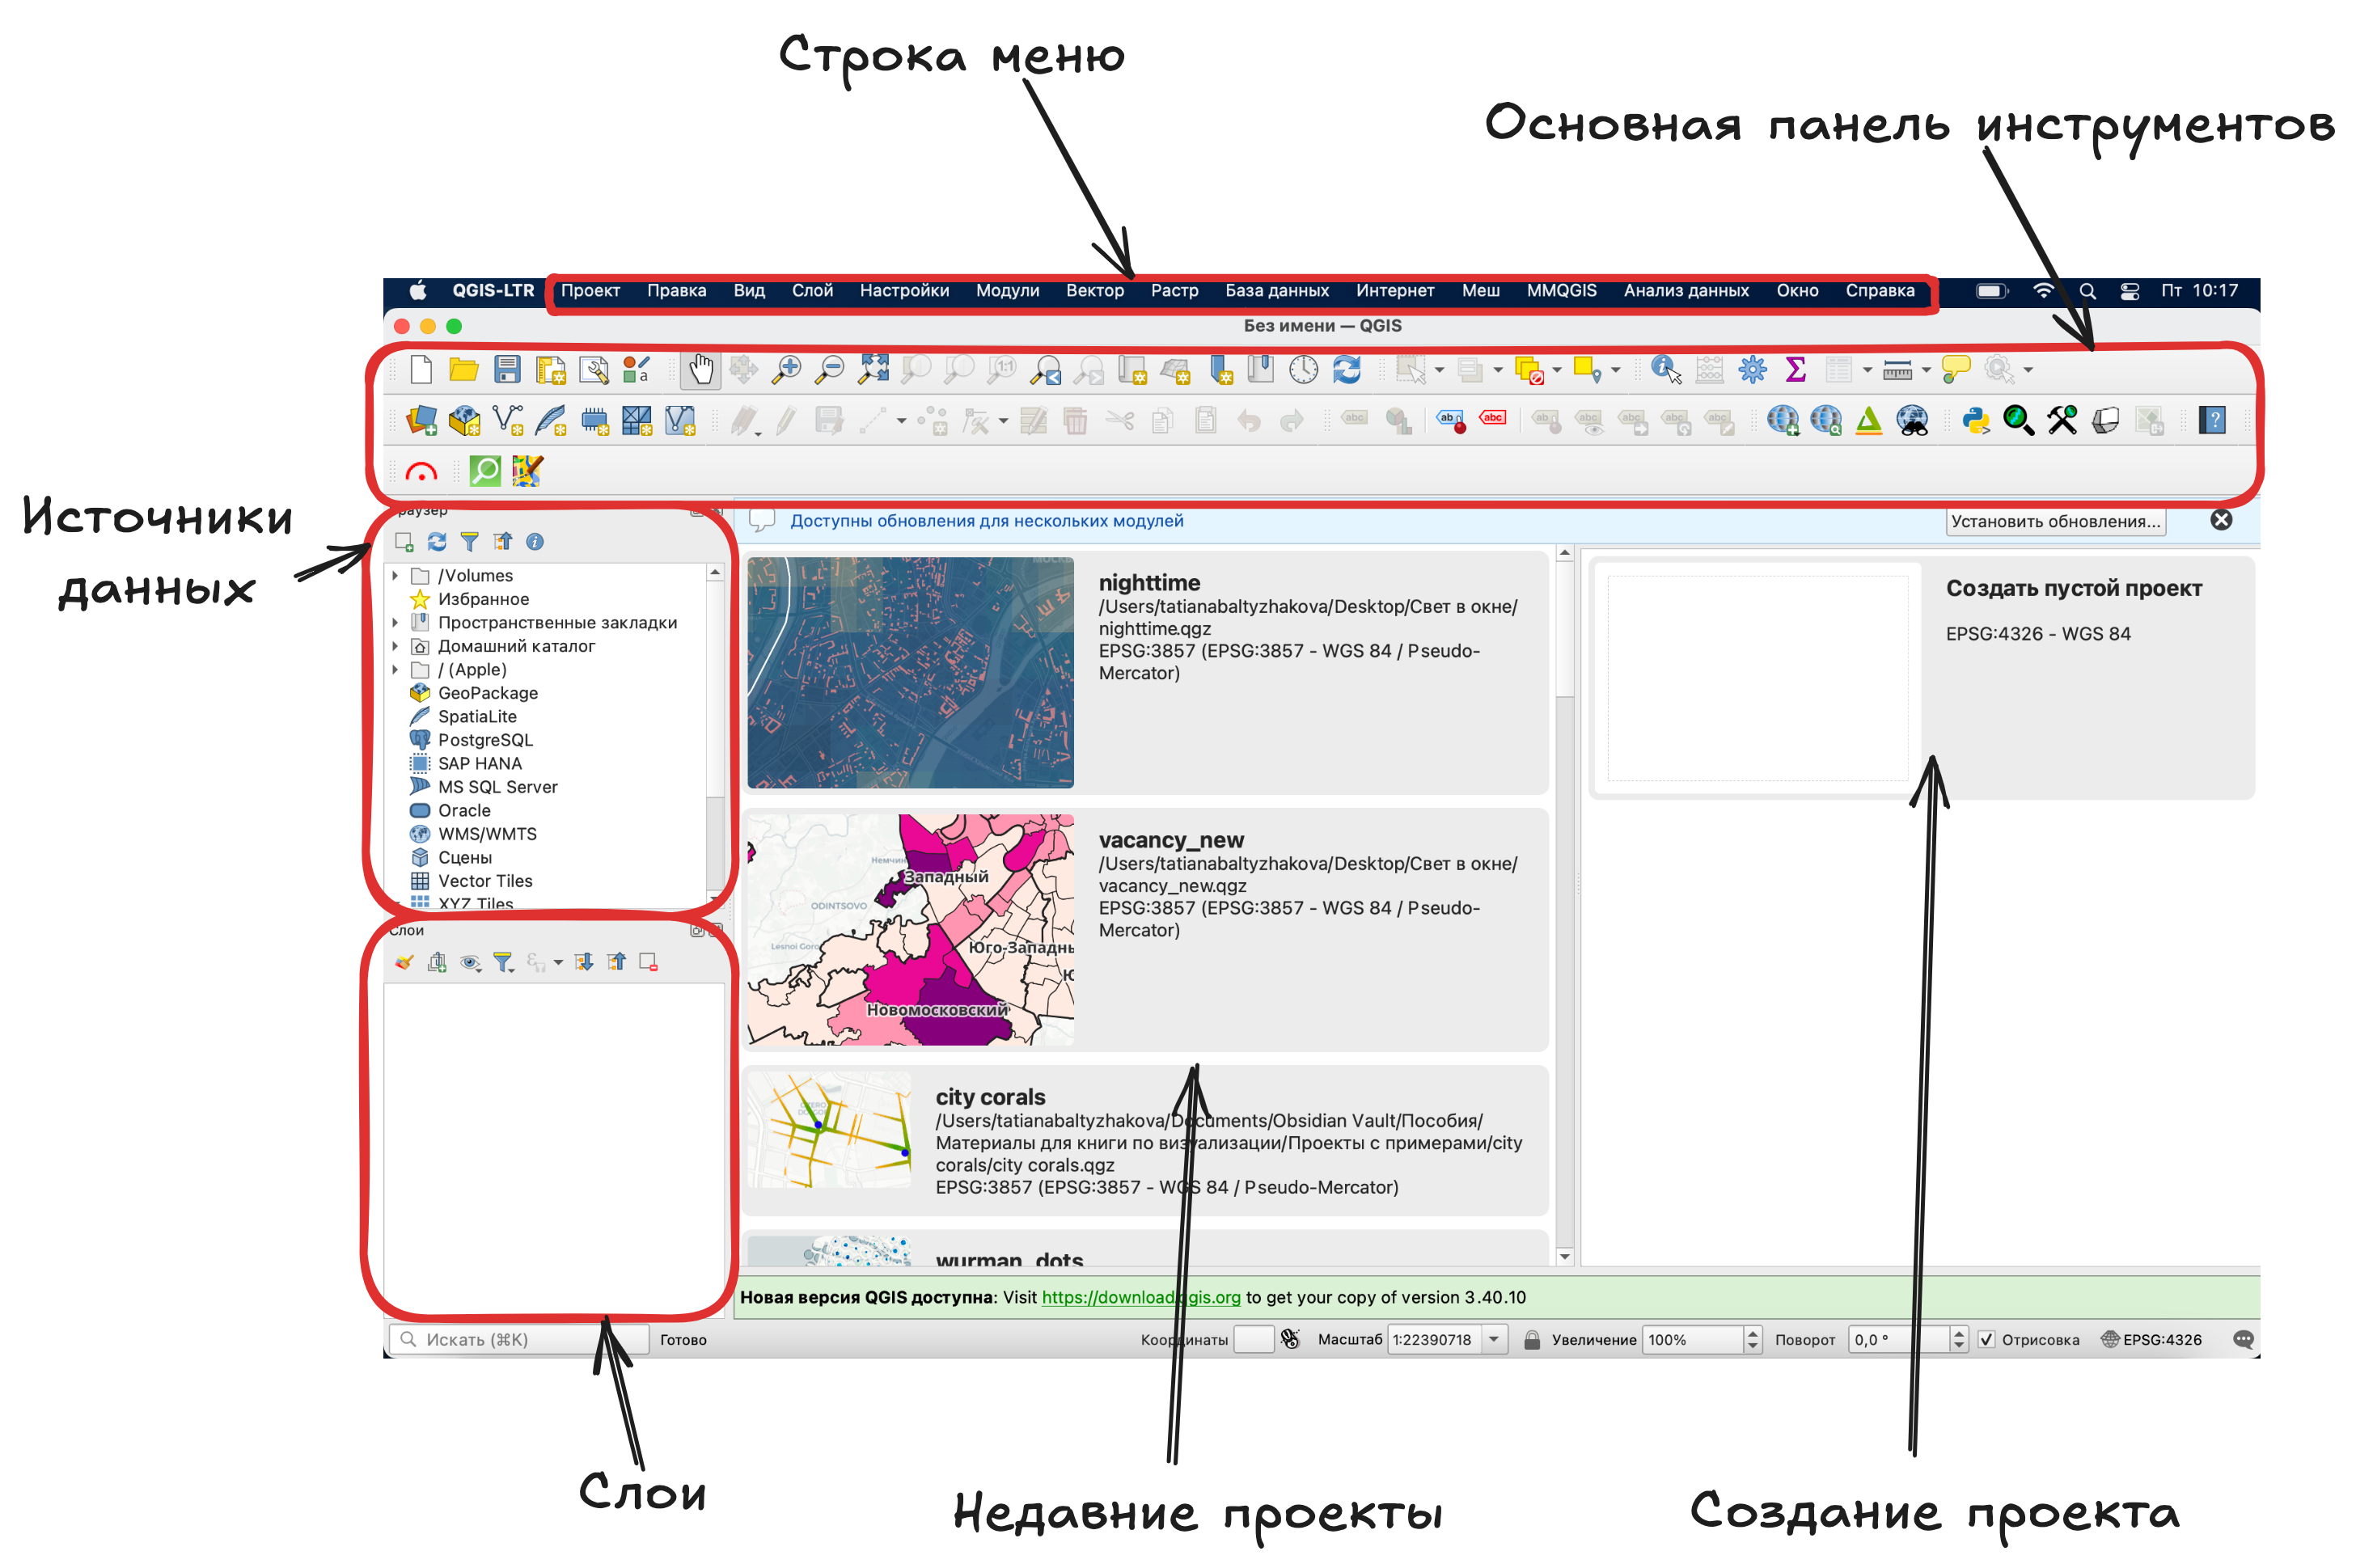
\includegraphics[keepaspectratio]{images/clipboard-2351392051.png}}
\end{center}

\begin{itemize}
\tightlist
\item
  панель \emph{Браузер} отображает все доступные вам источники данных
  как локальные (файлы на вашем компьютере), так и удаленные (базы
  данных и подключение к картографическим сервисам);
\end{itemize}

\begin{center}
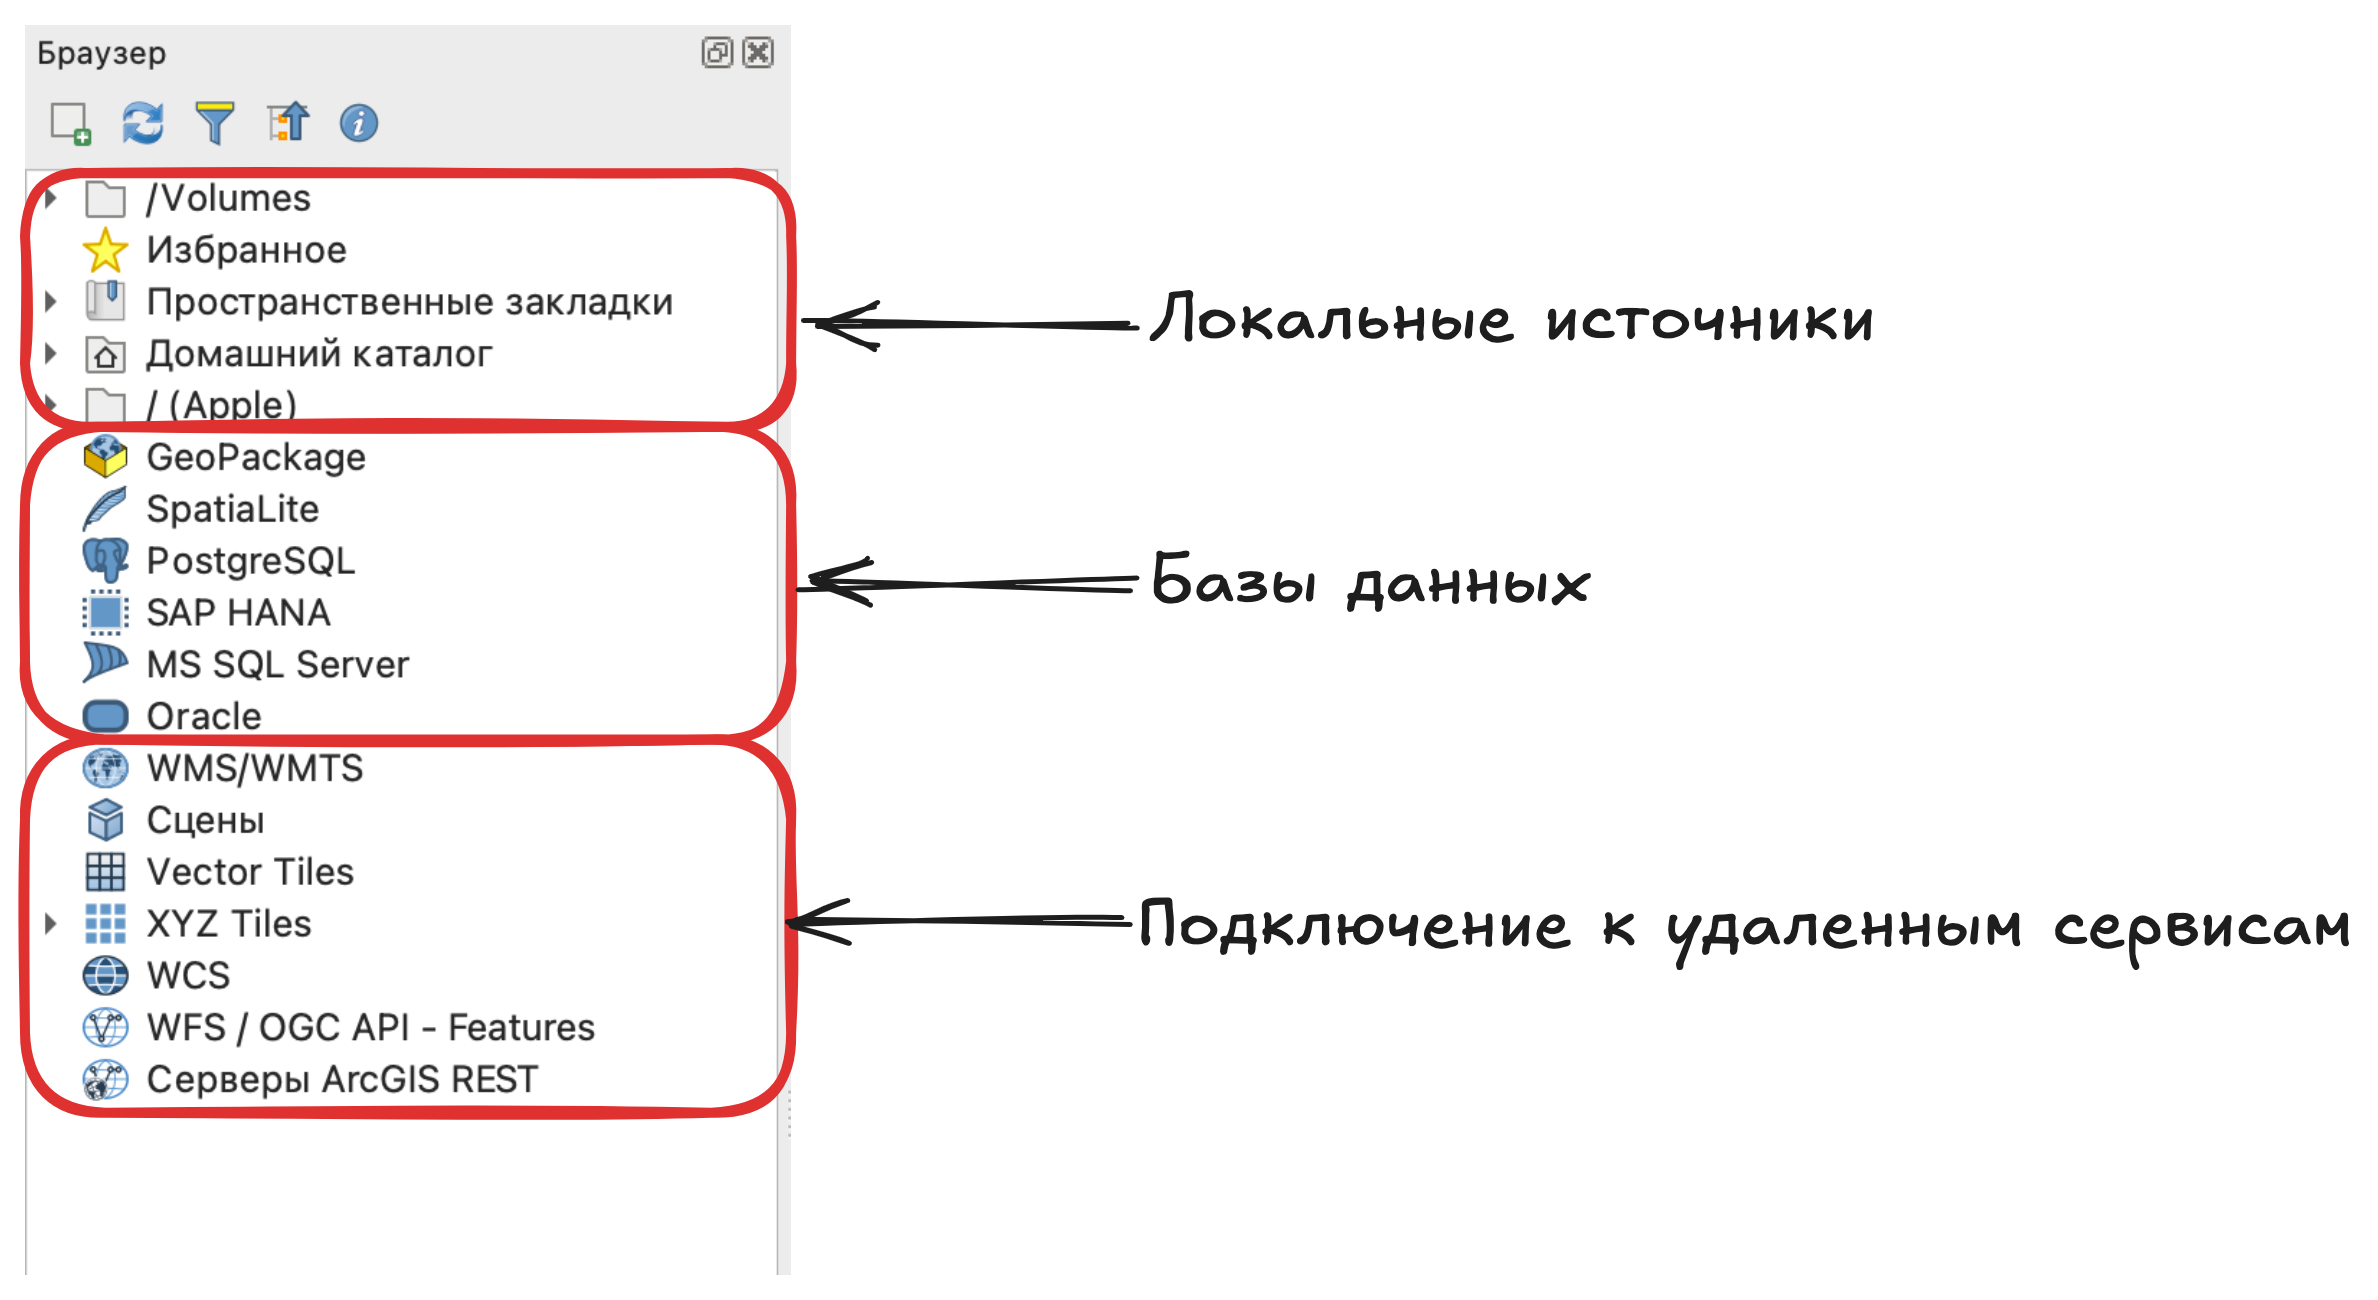
\includegraphics[width=6.80208in,height=\textheight,keepaspectratio]{images/clipboard-3652349245.png}
\end{center}

\begin{itemize}
\tightlist
\item
  панель \emph{Слои} будет отображать все открытые в данный момент слои
  вашего проекта.
\end{itemize}

Если вы закрыли панель браузера и/или панель слоев, то вы можете открыть
их снова из строки меню: \emph{Вид} \(\longrightarrow\) \emph{Панели}
\(\longrightarrow\) \emph{Браузер} или \emph{Слои}.

\begin{center}
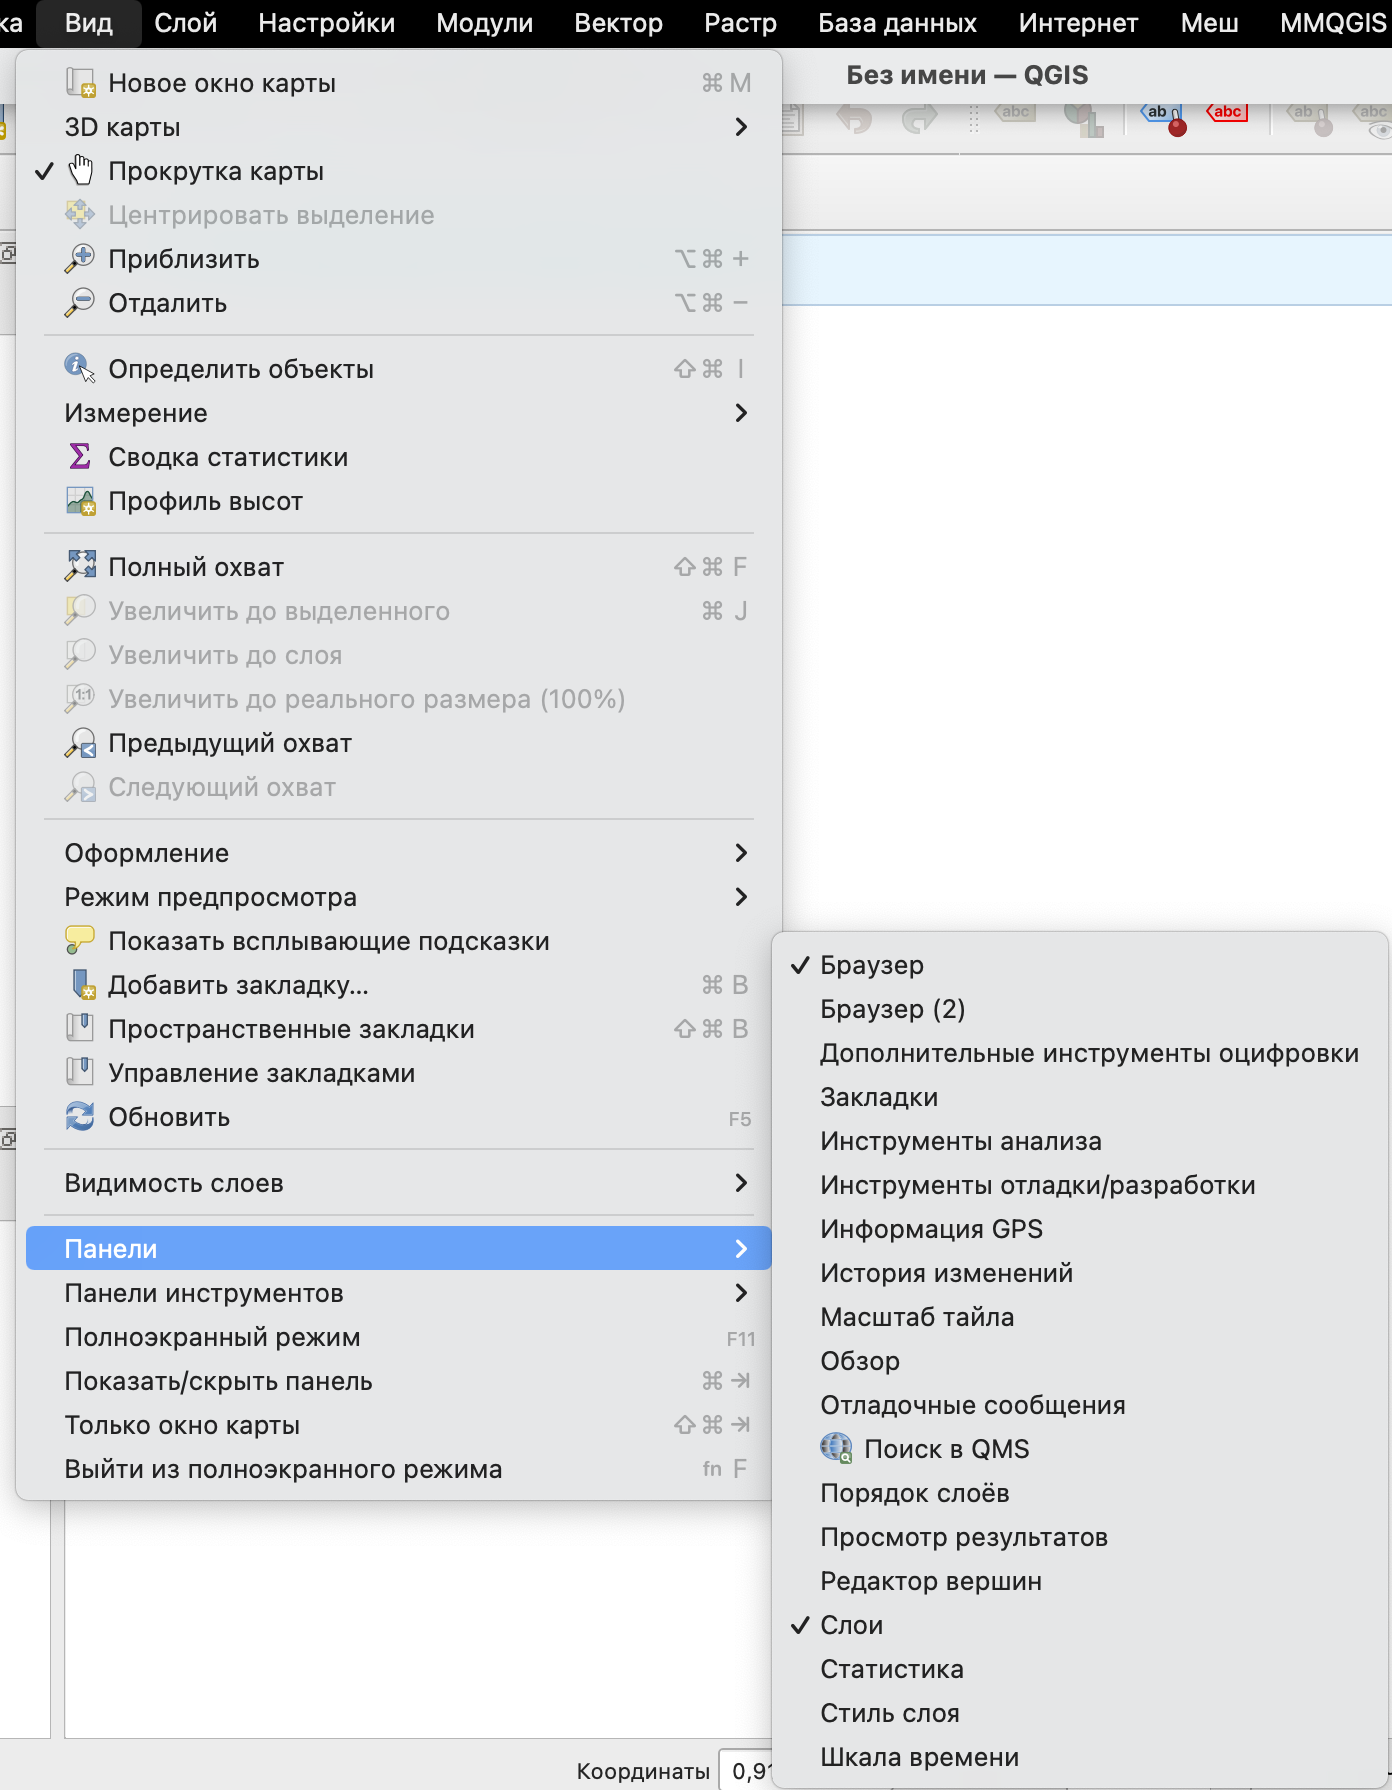
\includegraphics[width=6.47917in,height=\textheight,keepaspectratio]{images/clipboard-3478182616.png}
\end{center}

После того как вы создадите свой первый пустой проект вы увидите пустое
рабочее пространство, которое в некоторых контекстах и документации
может называться холстом.

\pandocbounded{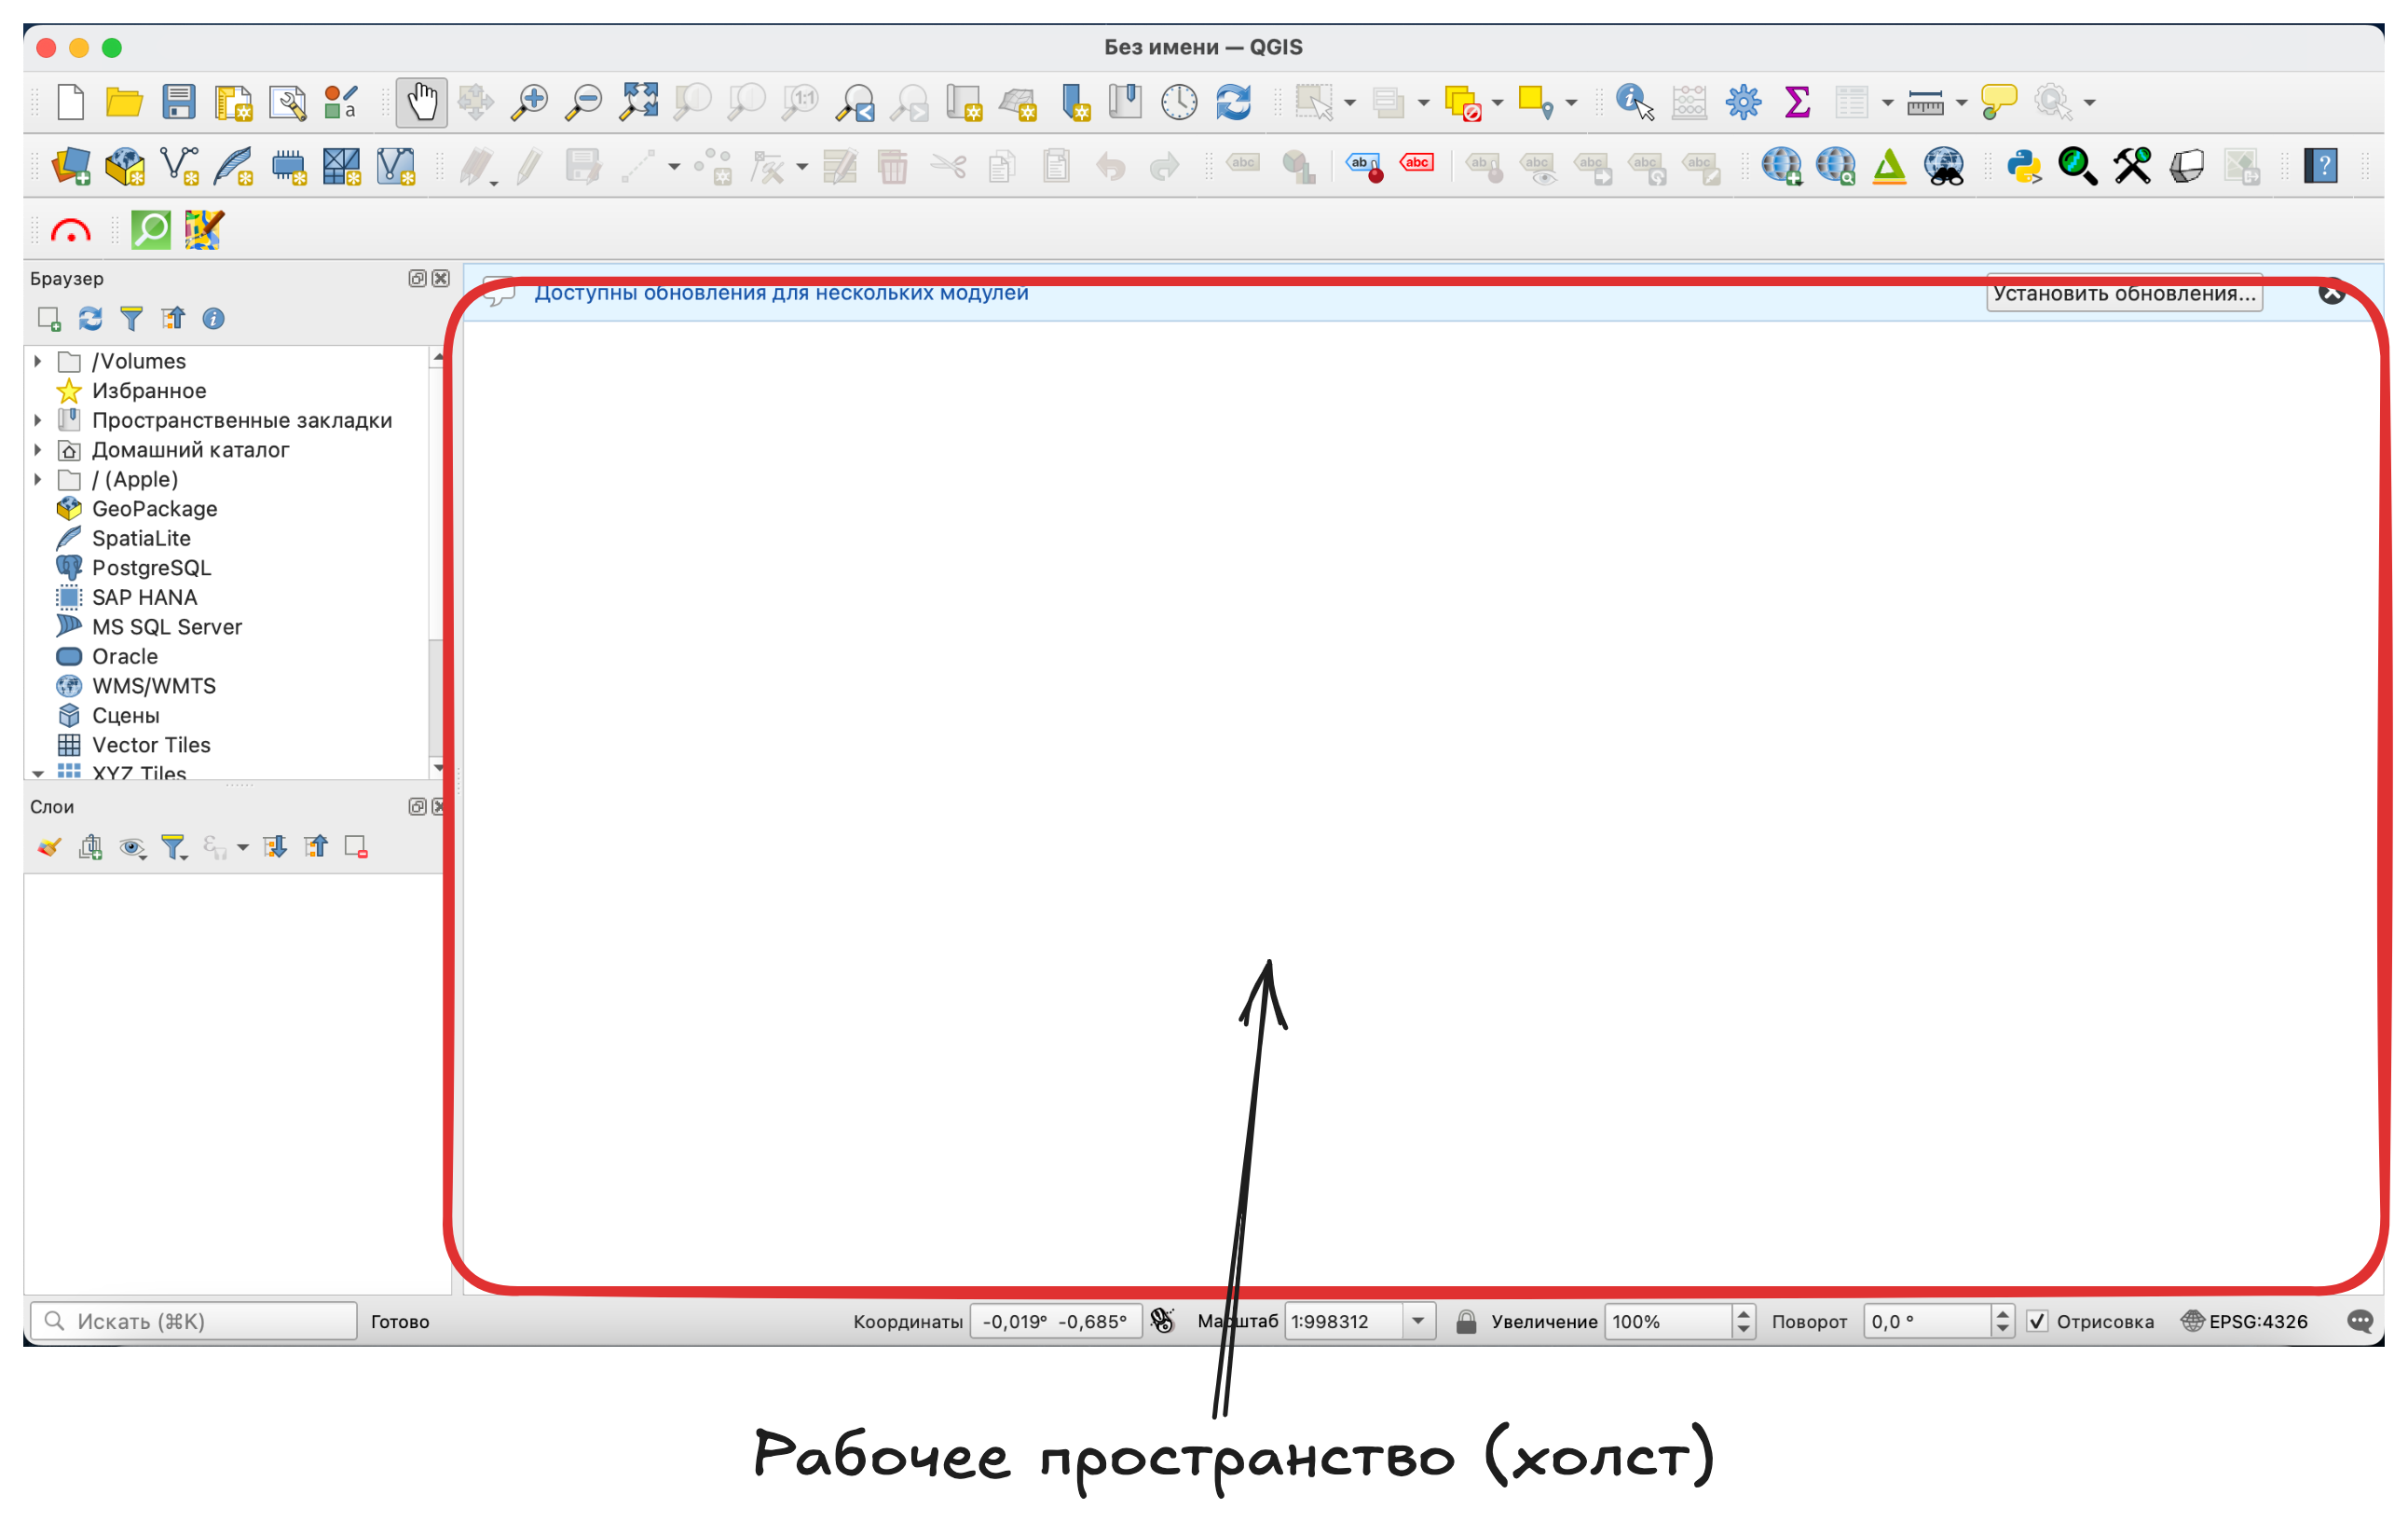
\includegraphics[keepaspectratio]{images/clipboard-1781010824.png}}

На основной панели инструментов, как правило, отображаются базовые
инструменты работы, некоторых из которых подписаны на картинке. Она
может дополняться как некоторыми инструментами из основного набора, так
и некоторыми инструментами из дополнительных модулей.

\pandocbounded{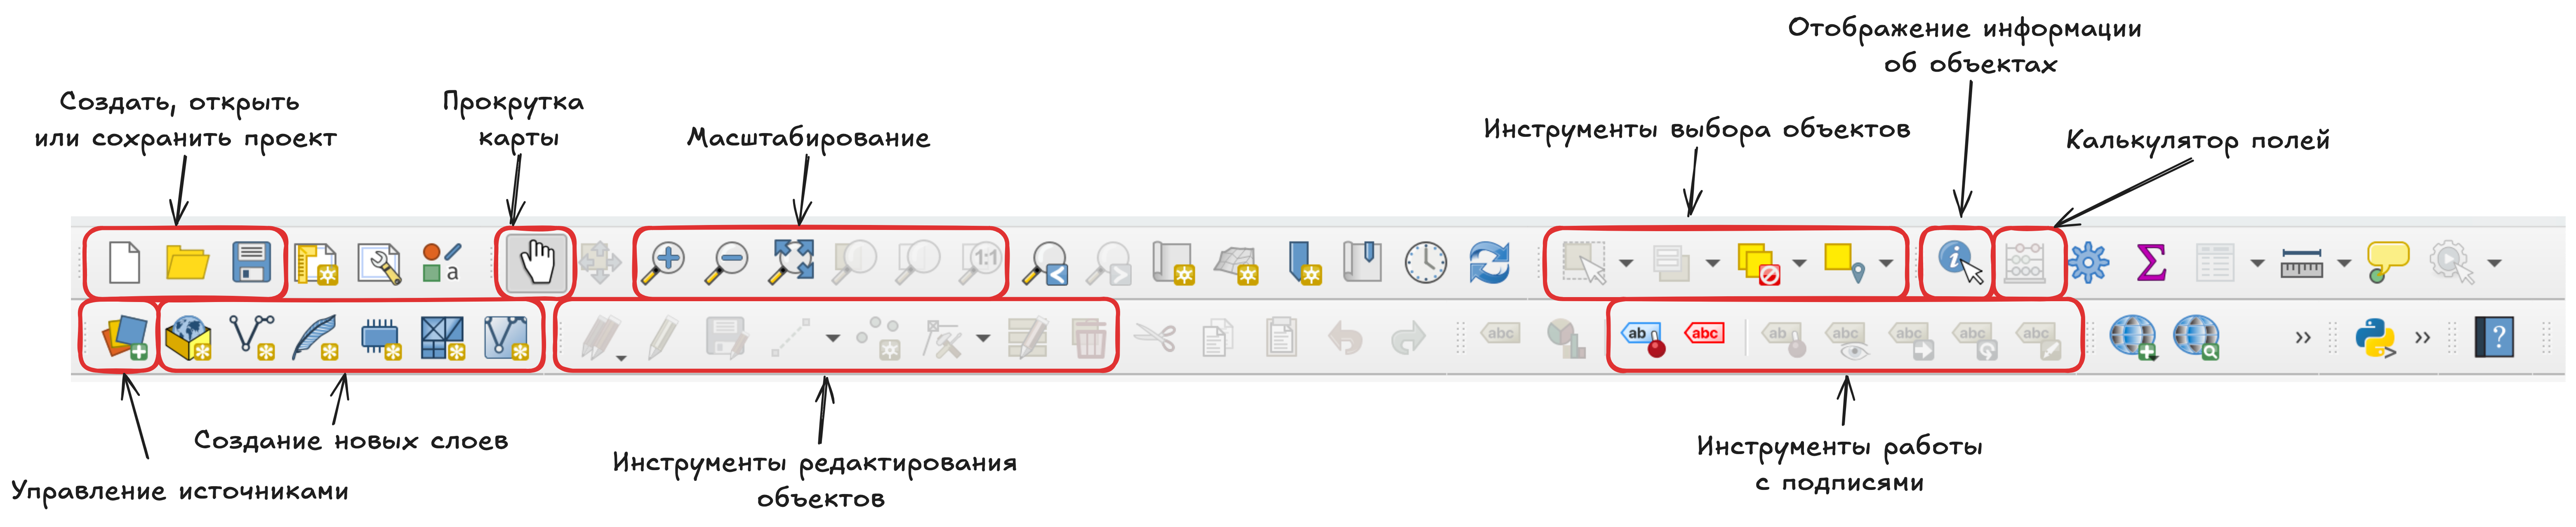
\includegraphics[keepaspectratio]{images/clipboard-3808504657.png}}

\begin{tcolorbox}[enhanced jigsaw, arc=.35mm, bottomrule=.15mm, bottomtitle=1mm, breakable, colback=white, colbacktitle=quarto-callout-tip-color!10!white, colframe=quarto-callout-tip-color-frame, coltitle=black, left=2mm, leftrule=.75mm, opacityback=0, opacitybacktitle=0.6, rightrule=.15mm, title=\textcolor{quarto-callout-tip-color}{\faLightbulb}\hspace{0.5em}{Дополнительно}, titlerule=0mm, toprule=.15mm, toptitle=1mm]

Что такое модуль?

Это либо дополнительные инструменты для расчетов, которых нет в базовом
наборе, либо инструменты, предоставляющие возможность взаимодействия с
удаленными источниками (например, загрузка данных).

\end{tcolorbox}

В нижней части окна есть некоторые дополнительные инструменты
взаимодействия с рабочим пространством.

\pandocbounded{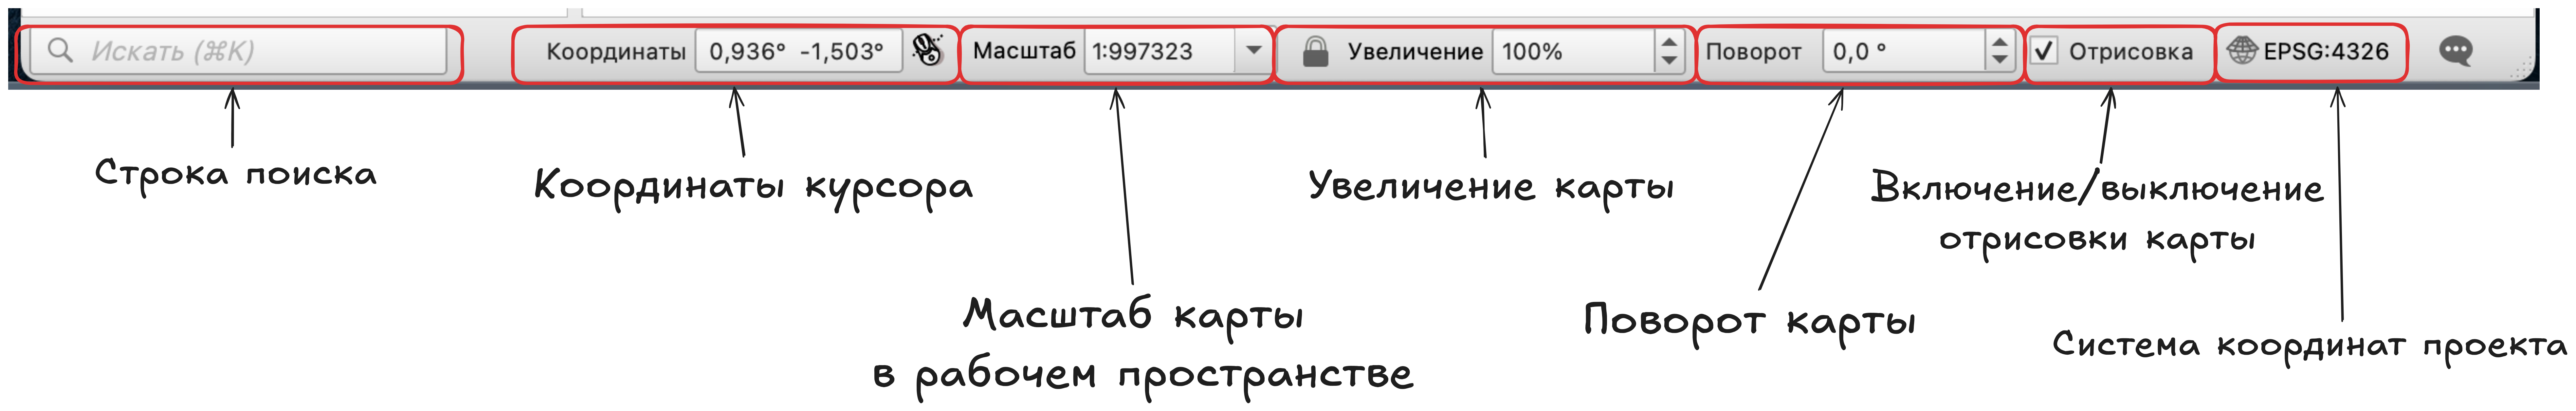
\includegraphics[keepaspectratio]{images/clipboard-1991001506.png}}

\begin{itemize}
\item
  строка поиска позволяет искать искать объекты по названию\footnote{\url{https://docs.qgis.org/3.40/en/docs/user_manual/introduction/qgis_gui.html\#locator-bar}};
\item
  далее показаны координаты вашего указателя мыши в системе координат
  проекта, по клику на значок мыши справа вы можете переключить эту
  строку в режим отображения охвата (то есть минимальных и максимальных
  координат видимой в рабочем пространстве карты)\footnote{здесь
    заложены некоторые ``пасхалки'' от разработчиков, почитать про них
    можно (на англ.)
    \url{https://www.geographyrealm.com/qgis-easter-eggs/} или (на
    русском) \url{https://cartetika.ru/tpost/1h9c4oc5o1-pashalki-v-qgis}};
\item
  масштаб, который может быть выбран из линейки стандартных (из
  выпадающего списка) или задан числом с клавиатуры;
\item
  увеличение позволяет увеличить изображение видимого фрагмента карты
  без изменения масштаба (как увеличительное стекло), требует фиксации
  масштаба кликом на значок замка;
\item
  поворот карты, который задается в градусах по часовой стрелке от
  направление на север;
\item
  включенная опция отрисовки карты значит, что изображение видимого в
  рабочем пространстве фрагмента карты будет меняться при перемещении
  и/или масштабировании, если вы ее отключите, то зафиксируете
  содержание карты;
\item
  система координат проекта.
\end{itemize}

\begin{tcolorbox}[enhanced jigsaw, arc=.35mm, bottomrule=.15mm, bottomtitle=1mm, breakable, colback=white, colbacktitle=quarto-callout-important-color!10!white, colframe=quarto-callout-important-color-frame, coltitle=black, left=2mm, leftrule=.75mm, opacityback=0, opacitybacktitle=0.6, rightrule=.15mm, title=\textcolor{quarto-callout-important-color}{\faExclamation}\hspace{0.5em}{Важно}, titlerule=0mm, toprule=.15mm, toptitle=1mm]

Система координат проекта в первую очередь задает систему координат для
той карты, которую мы видим в основном рабочем пространстве, кроме того,
в ней могут осуществляться некоторые расчеты (в зависимости от
инструмента).

Эта система координат не зависит от систем координат слоев и считается
внешней для них.

\end{tcolorbox}

\section{Добавление подложки на
карту}\label{ux434ux43eux431ux430ux432ux43bux435ux43dux438ux435-ux43fux43eux434ux43bux43eux436ux43aux438-ux43dux430-ux43aux430ux440ux442ux443}

Для начала работы добавим в наш проект подложку.

Подложкой в ГИС называют то, что используется как фоновое изображение,
как правило, это может быть карта в виде тайлов или какое-либо
изображение (спутниковый снимок, растр с геопривязкой).

Подложка необходима для добавления контекста на карту, возможности
ориентирования на местности, а также она может выполнять эстетическую
функцию при подготовке и оформлении карт.

По умолчанию на панели браузер нам доступны два варианта подложек в
формате \textbf{XYZ Tiles}:

\begin{itemize}
\item
  \emph{OpenStreetMap} - подложка на основе данных OpenStreet Map;
\item
  \emph{Mapzen Global Terrain} - подложка на основе сведений о рельефе.
\end{itemize}

По двойному клику левой кнопкой мыши вы можете добавить любую из них.

\pandocbounded{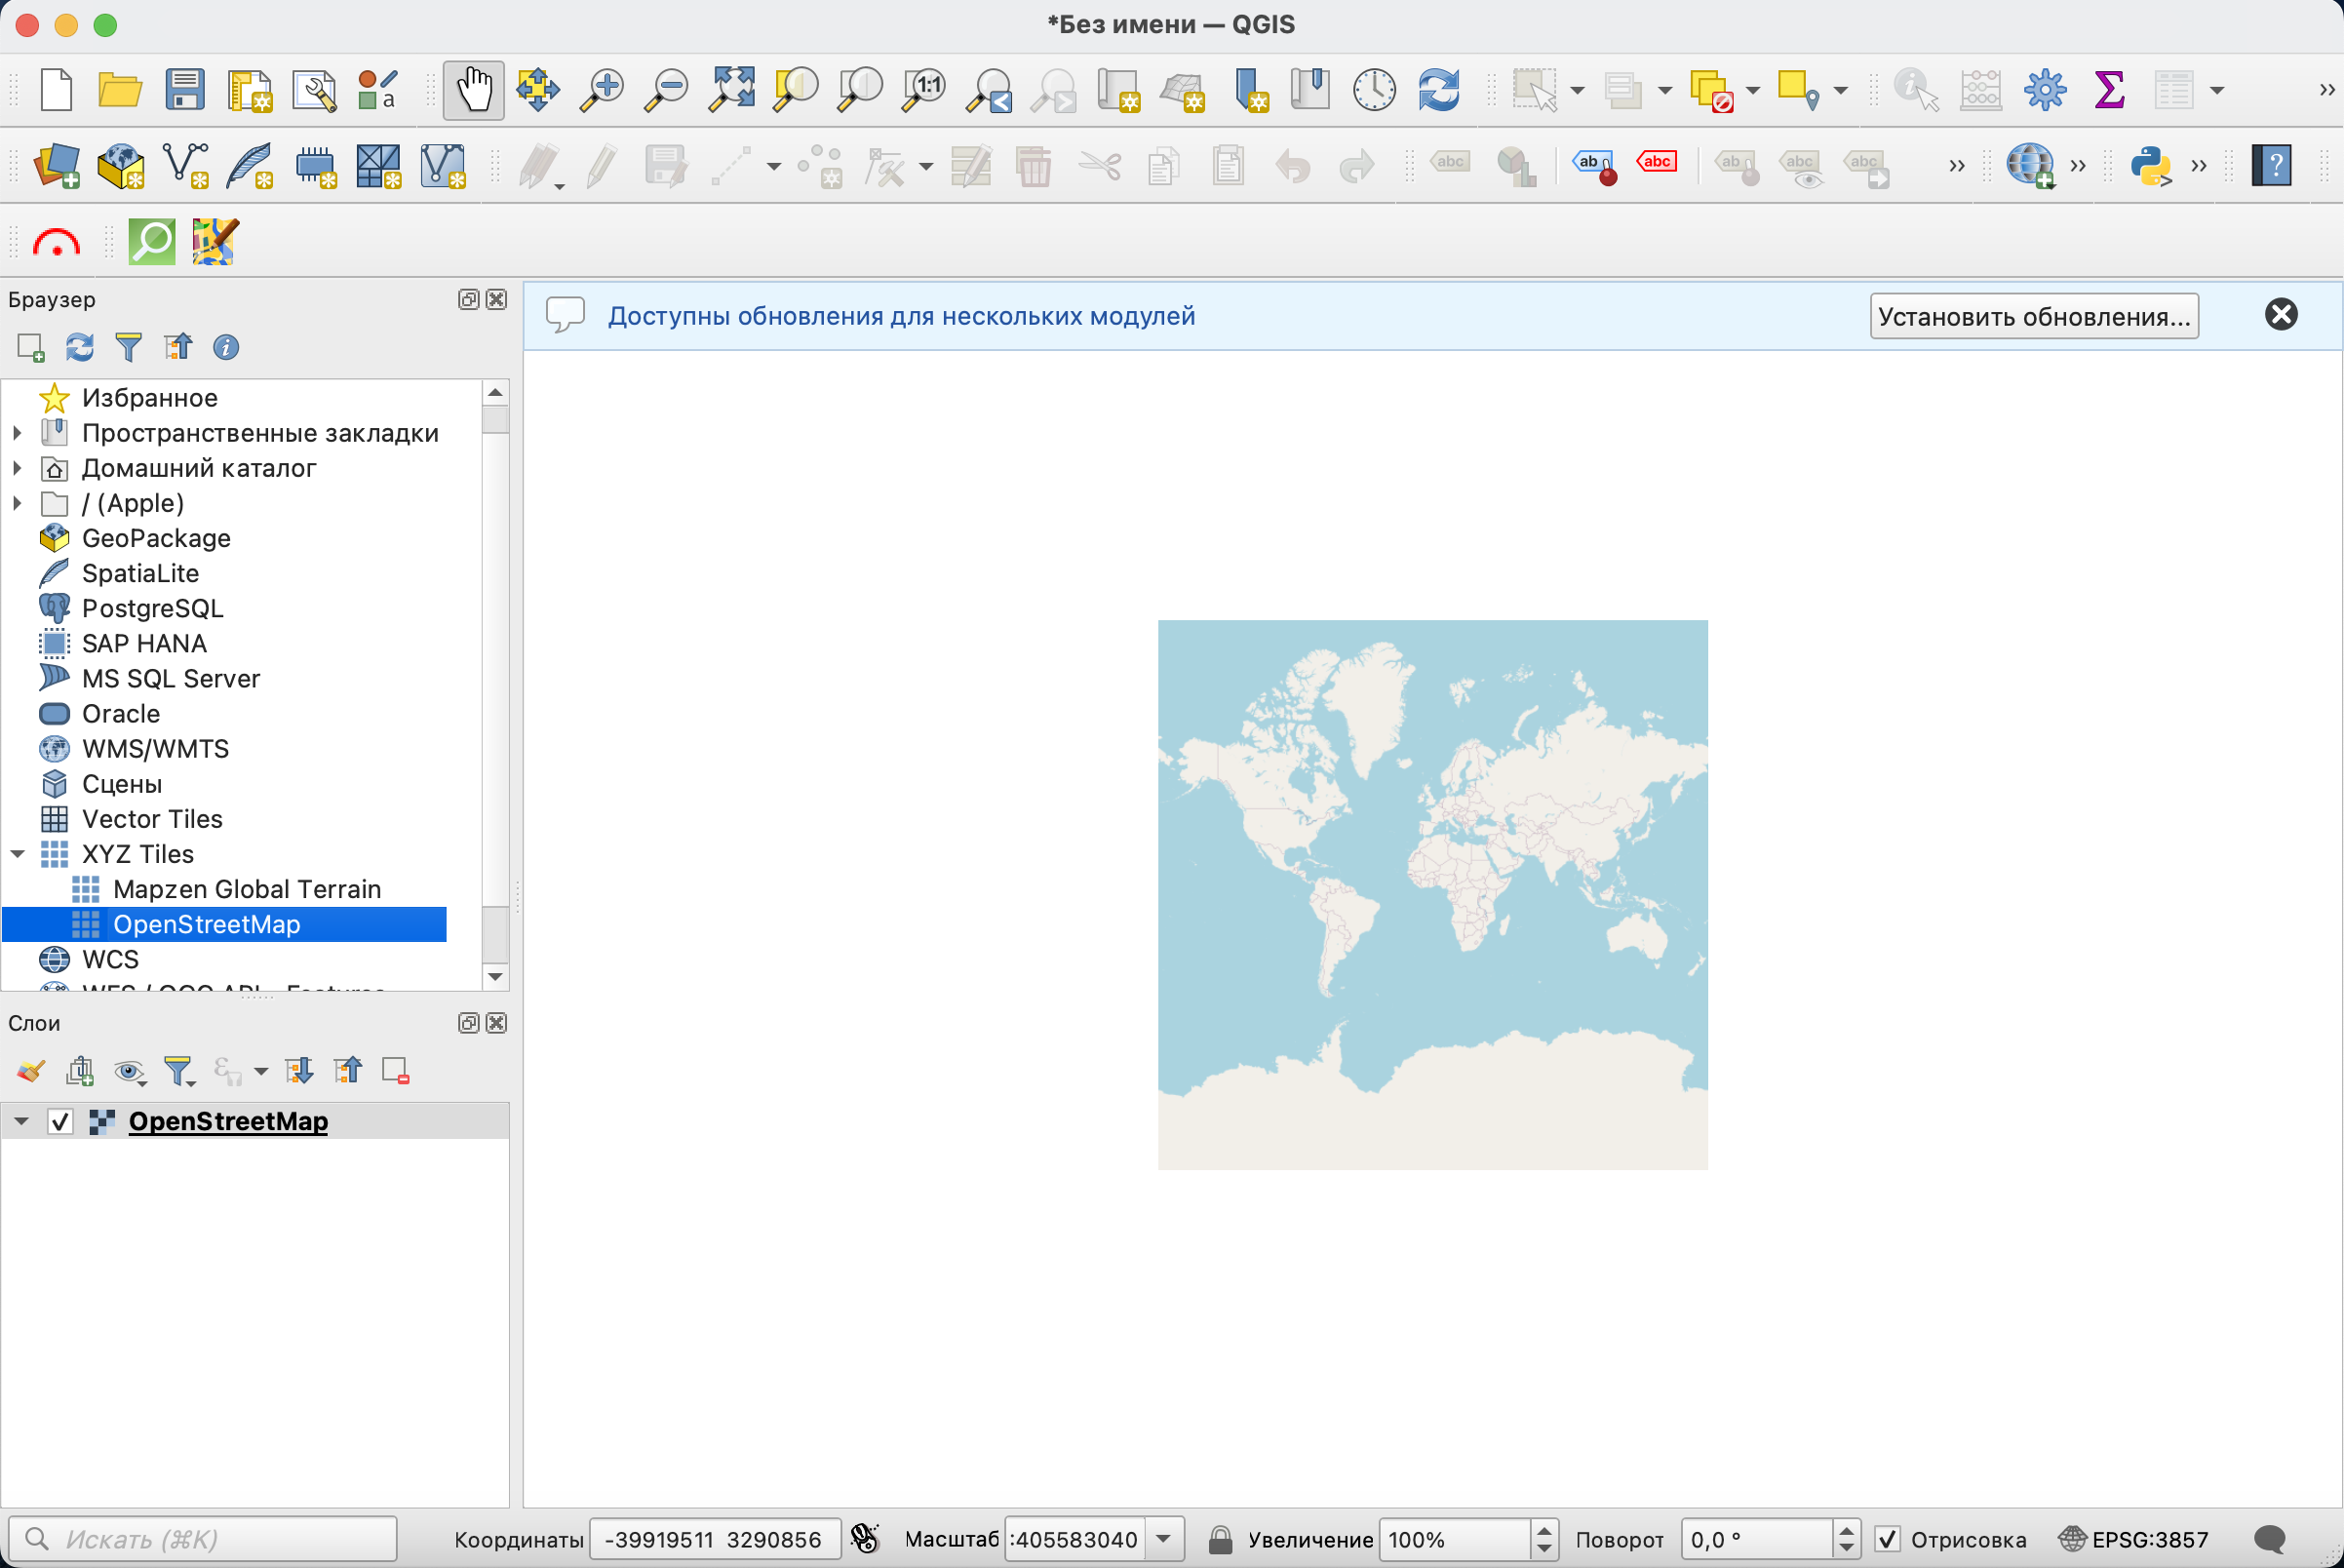
\includegraphics[keepaspectratio]{images/clipboard-2123566421.png}}

После добавления она должна появиться в рабочем пространстве и в панели
слоев.

Обратите внимание, что слева от названия подложки в панели слоев
нарисован квадратик с разноцветными ячейками, это значит, что
\textbf{слой растровый}.

\begin{tcolorbox}[enhanced jigsaw, arc=.35mm, bottomrule=.15mm, bottomtitle=1mm, breakable, colback=white, colbacktitle=quarto-callout-tip-color!10!white, colframe=quarto-callout-tip-color-frame, coltitle=black, left=2mm, leftrule=.75mm, opacityback=0, opacitybacktitle=0.6, rightrule=.15mm, title=\textcolor{quarto-callout-tip-color}{\faLightbulb}\hspace{0.5em}{Дополнительно}, titlerule=0mm, toprule=.15mm, toptitle=1mm]

При необходимости вы можете сами создавать и настраивать подключения к
картографическим сервисам.

\end{tcolorbox}

\subsection{Модуль
QuickMapServices}\label{ux43cux43eux434ux443ux43bux44c-quickmapservices}

Если подложек по умолчанию вам недостаточно, то вы можете как настроить
новые подключения к другим сервисам, так и воспользоваться модулем
(плагином) \textbf{QuickMapServices}, который предназначен для
добавления геосервисов и базовых карт.

Информацию о всех доступных модулях вы можете посмотреть на официальном
сайте репозитория - \url{https://plugins.qgis.org/}

Для установки модуля в строке меню нужно выбрать \emph{Модули}
\(\longrightarrow\) \emph{Управление модулями}, после чего вы увидите
окно репозитория (возможно понадобится пара секунд, чтобы в нему
подключиться), в котором можно найти интересующий вас модуль и
установить.

\begin{center}
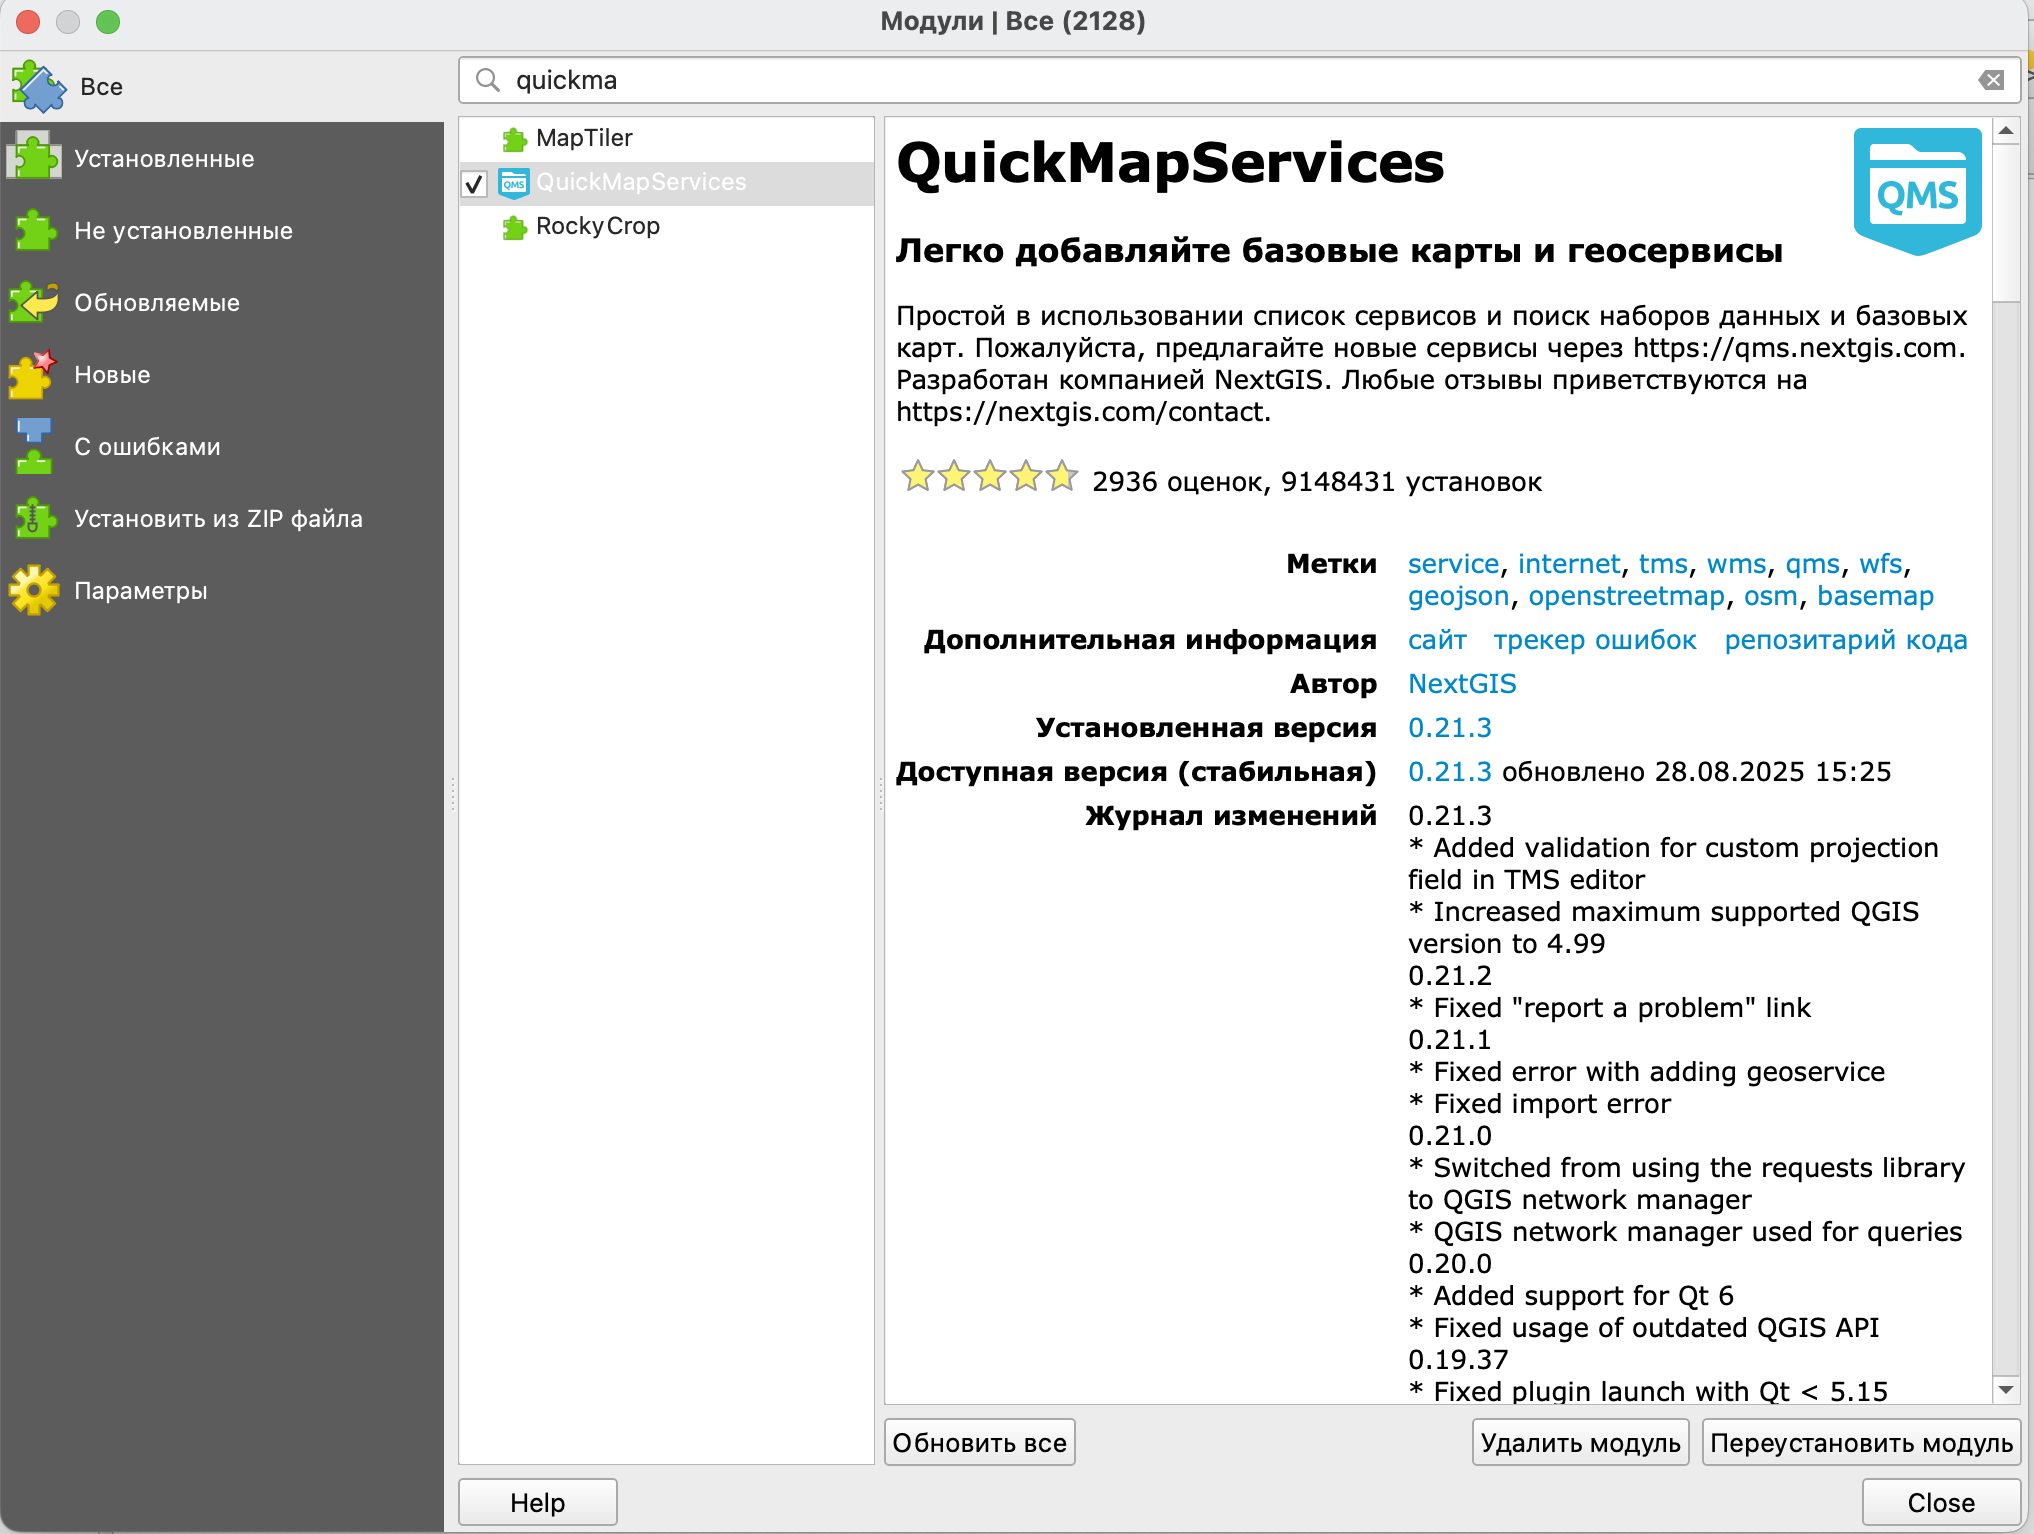
\includegraphics[width=12.42708in,height=\textheight,keepaspectratio]{images/clipboard-3226047774.png}
\end{center}

В том случае, если по какой-то причине вы не можете подключиться
напрямую к репозиторию из программы и установить нужный вам модуль, вы
можете скачать архив с модулем с сайта \url{https://plugins.qgis.org/} и
установить его, воспользовавшись опцией \emph{Установить из ZIP файла}.

После успешной установки модуля у вас в правой части окна появится
панель поиска геосервисов, где вы можете искать их по текстовому
запросу.

\begin{center}
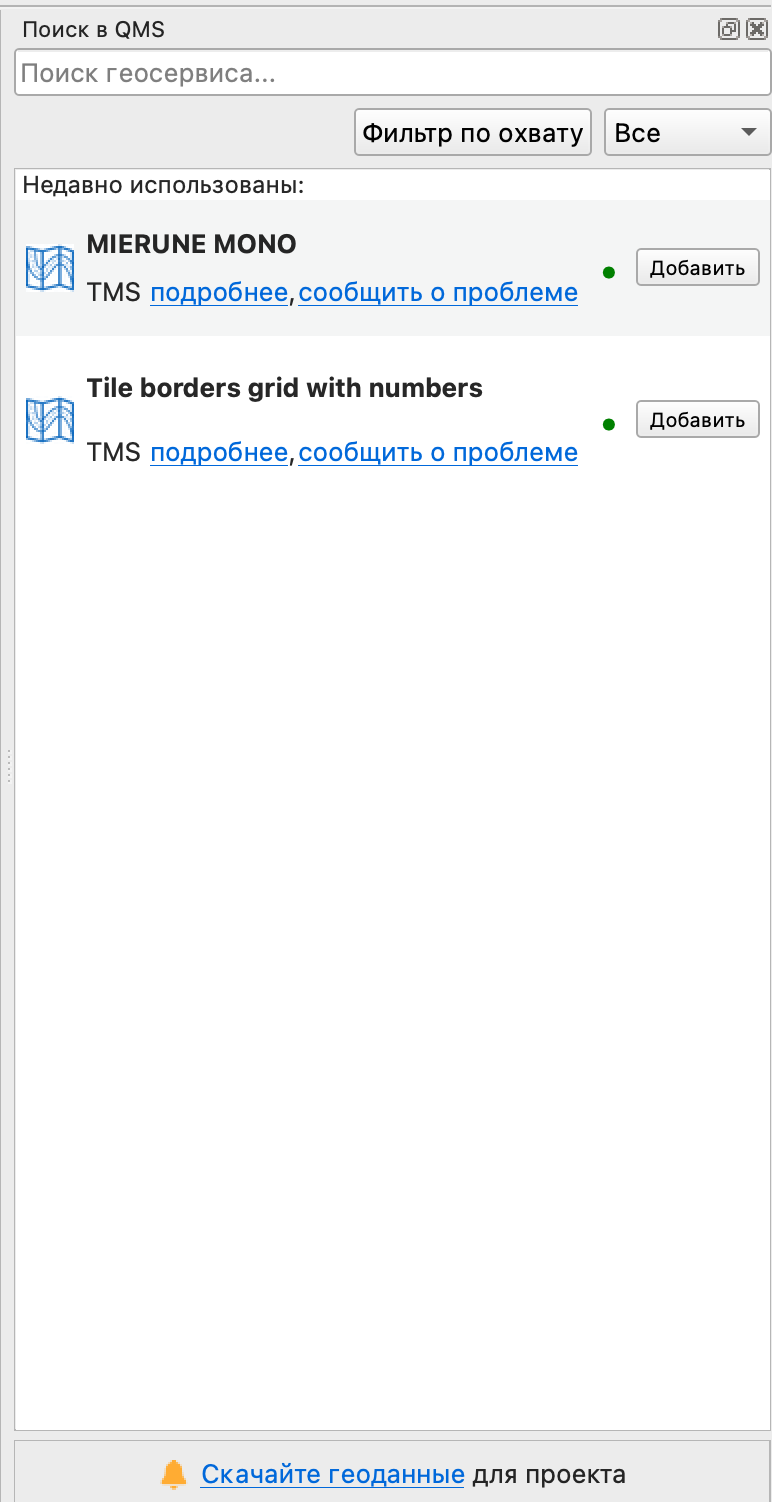
\includegraphics[width=4.82292in,height=\textheight,keepaspectratio]{images/clipboard-2328006450.png}
\end{center}

Если вы не хотите этого делать, панель можно просто закрыть.

Также на вашей основной панели инструментов должен появиться значок

\includegraphics[width=0.53125in,height=\textheight,keepaspectratio]{images/clipboard-522767533.png},
по клику на который вы увидите перечень доступных вам геосервисов и
базовых карт.

\begin{center}
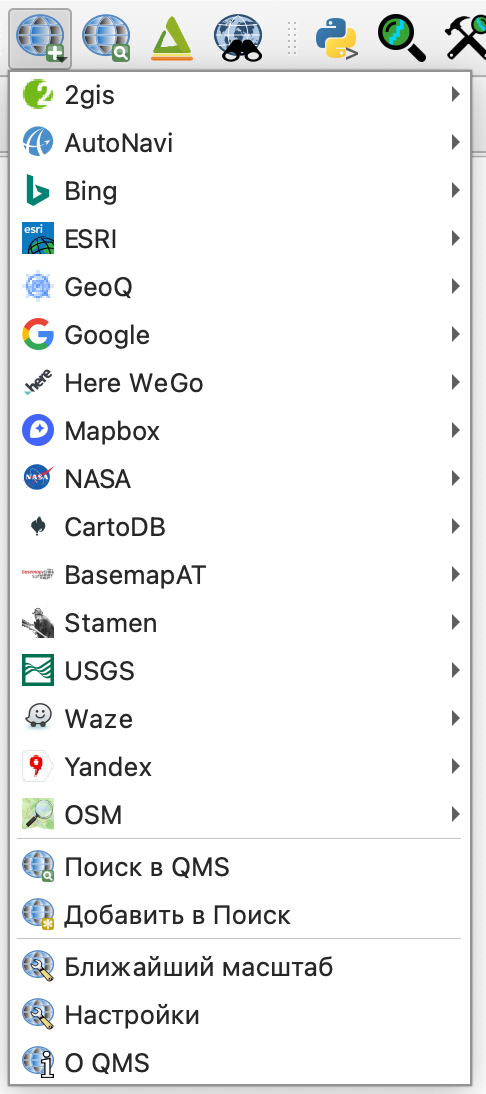
\includegraphics[width=3.69792in,height=\textheight,keepaspectratio]{images/clipboard-925549371.png}
\end{center}

\begin{tcolorbox}[enhanced jigsaw, arc=.35mm, bottomrule=.15mm, bottomtitle=1mm, breakable, colback=white, colbacktitle=quarto-callout-important-color!10!white, colframe=quarto-callout-important-color-frame, coltitle=black, left=2mm, leftrule=.75mm, opacityback=0, opacitybacktitle=0.6, rightrule=.15mm, title=\textcolor{quarto-callout-important-color}{\faExclamation}\hspace{0.5em}{Важно}, titlerule=0mm, toprule=.15mm, toptitle=1mm]

При первой установке модуля у вас не будет такого большого перечня, как
показано на картинке. Если вы хотите открыть к нему доступ, то вам нужно
перейти в настройки модуля и открыть вкладку \emph{Загрузить сервисы}
(\emph{Load more services}).

В этом окне вам нужно нажать на кнопку \emph{Получить дополнительные
источники данных} (\emph{Get contributed pack}), согласиться с условиями
их предоставления и сохранить настройки.

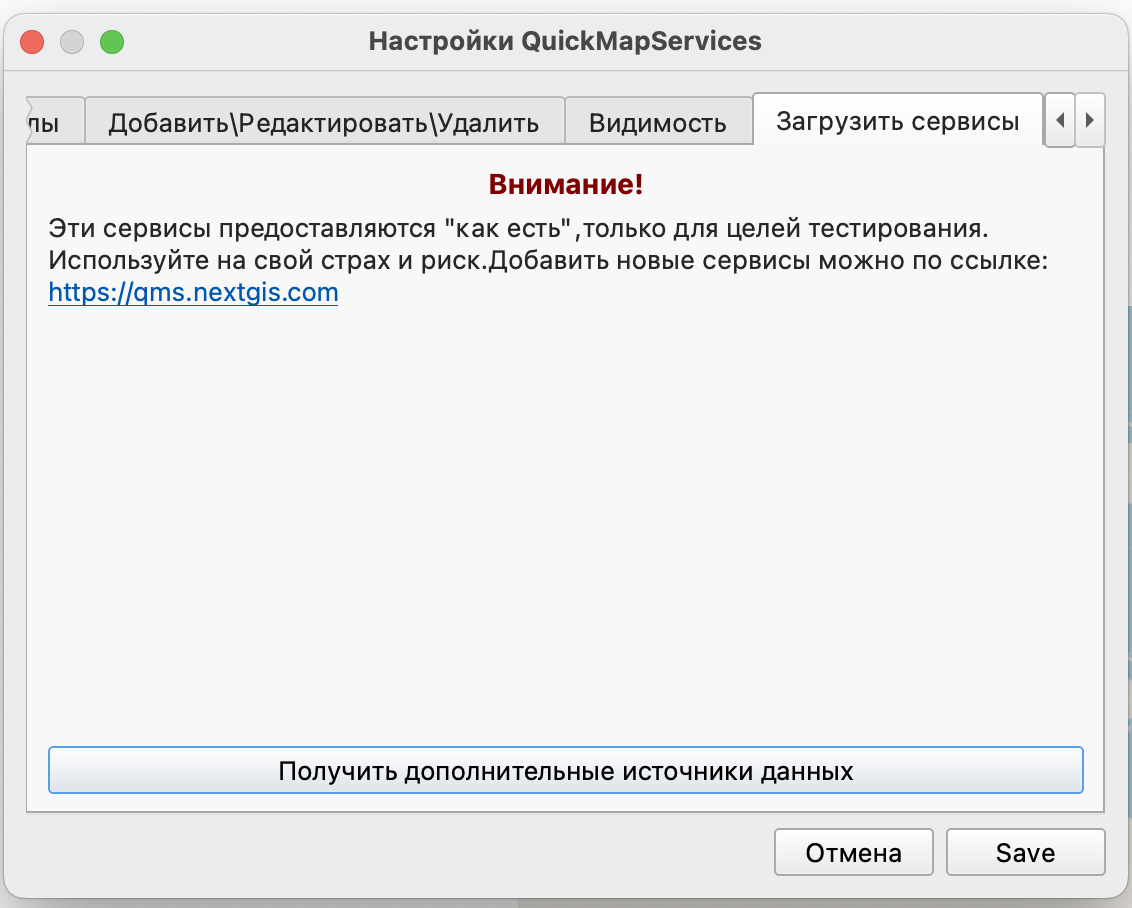
\includegraphics[width=10.38542in,height=\textheight,keepaspectratio]{images/clipboard-3228789104.png}

\end{tcolorbox}

\begin{tcolorbox}[enhanced jigsaw, arc=.35mm, bottomrule=.15mm, bottomtitle=1mm, breakable, colback=white, colbacktitle=quarto-callout-tip-color!10!white, colframe=quarto-callout-tip-color-frame, coltitle=black, left=2mm, leftrule=.75mm, opacityback=0, opacitybacktitle=0.6, rightrule=.15mm, title=\textcolor{quarto-callout-tip-color}{\faLightbulb}\hspace{0.5em}{Дополнительно}, titlerule=0mm, toprule=.15mm, toptitle=1mm]

Со списком всех доступных сервисов можно ознакомиться по ссылке
\url{https://qms.nextgis.com/}

Для более подробного ознакомления можете воспользоваться видео от
разработчиков.

Кроме того, что вы можете пользоваться уже имеющимися в модуле
подложками, можно подключать другие источники данных. Пример показан на
видео.

\begin{Shaded}
\begin{Highlighting}[]
\DataTypeTok{\textless{}}\KeywordTok{iframe}\OtherTok{ width}\OperatorTok{=}\StringTok{"720"}\OtherTok{ height}\OperatorTok{=}\StringTok{"405"}\OtherTok{ src}\OperatorTok{=}\StringTok{"https://rutube.ru/play/embed/a0926f5ac3c470563b2b39a12c47dfff/"}\OtherTok{ style}\OperatorTok{=}\StringTok{"border: none;"}\OtherTok{ allow}\OperatorTok{=}\StringTok{"clipboard{-}write; autoplay"}\OtherTok{ allowFullScreen}\DataTypeTok{\textgreater{}\textless{}/}\KeywordTok{iframe}\DataTypeTok{\textgreater{}}
\end{Highlighting}
\end{Shaded}

\end{tcolorbox}

\begin{tcolorbox}[enhanced jigsaw, arc=.35mm, bottomrule=.15mm, bottomtitle=1mm, breakable, colback=white, colbacktitle=quarto-callout-tip-color!10!white, colframe=quarto-callout-tip-color-frame, coltitle=black, left=2mm, leftrule=.75mm, opacityback=0, opacitybacktitle=0.6, rightrule=.15mm, title=\textcolor{quarto-callout-tip-color}{\faLightbulb}\hspace{0.5em}{Дополнительно}, titlerule=0mm, toprule=.15mm, toptitle=1mm]

Возможно после открытия новой подложки она появилась у вас в перечне
слоев, но не видна на карте, это происходит из-за того, что отрисовка
слоев ведется в том порядке, в котором они перечислены, то есть слои
ниже по списку находятся под более верхними слоями, которые их
закрывают.

При необходимости вы можете поменять порядок слоев, просто перетащив
один из них в списке выше или ниже, или отключить видимость верхнего
слоя, убрав галочку из чекбокса.

\end{tcolorbox}

\subsection{Настройка базовой
карты}\label{ux43dux430ux441ux442ux440ux43eux439ux43aux430-ux431ux430ux437ux43eux432ux43eux439-ux43aux430ux440ux442ux44b}

Так как базовые карты подложки у нас растровые, то настройка их стиля
довольно ограничена, хотя вы можете сделать так, чтобы они отвечали
общему стилю и задумке вашей карты.

Настройки стиля можно найти в свойствах слоя, которые открываются либо
двойным кликом по названию, либо из контекстного меню, полученного
кликом правой кнопки мыши.

\begin{center}
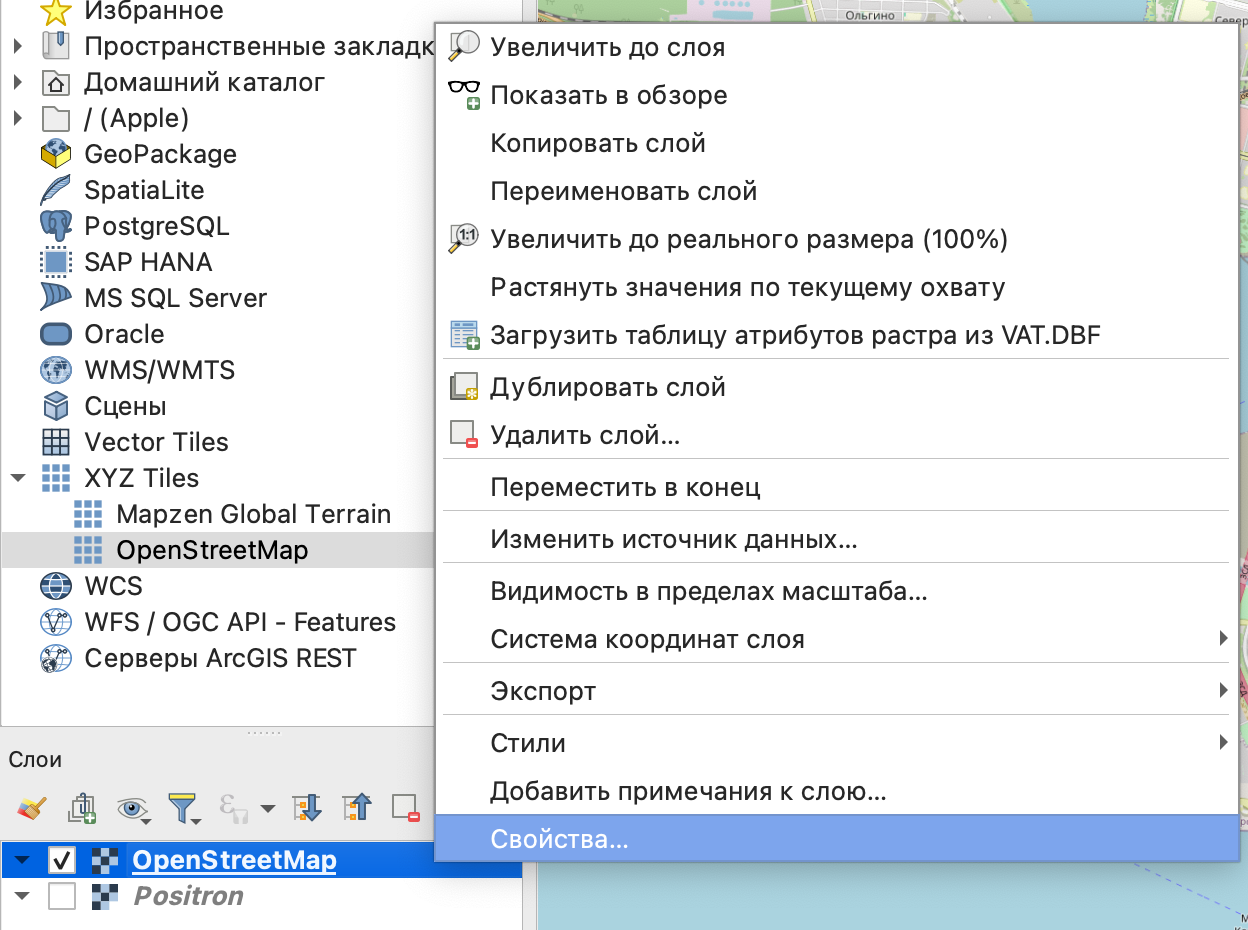
\includegraphics[width=9.78125in,height=\textheight,keepaspectratio]{images/clipboard-1308967251.png}
\end{center}

В свойствах вы увидите несколько пунктов, нас интересует пункт
\emph{Стиль}.

\begin{center}
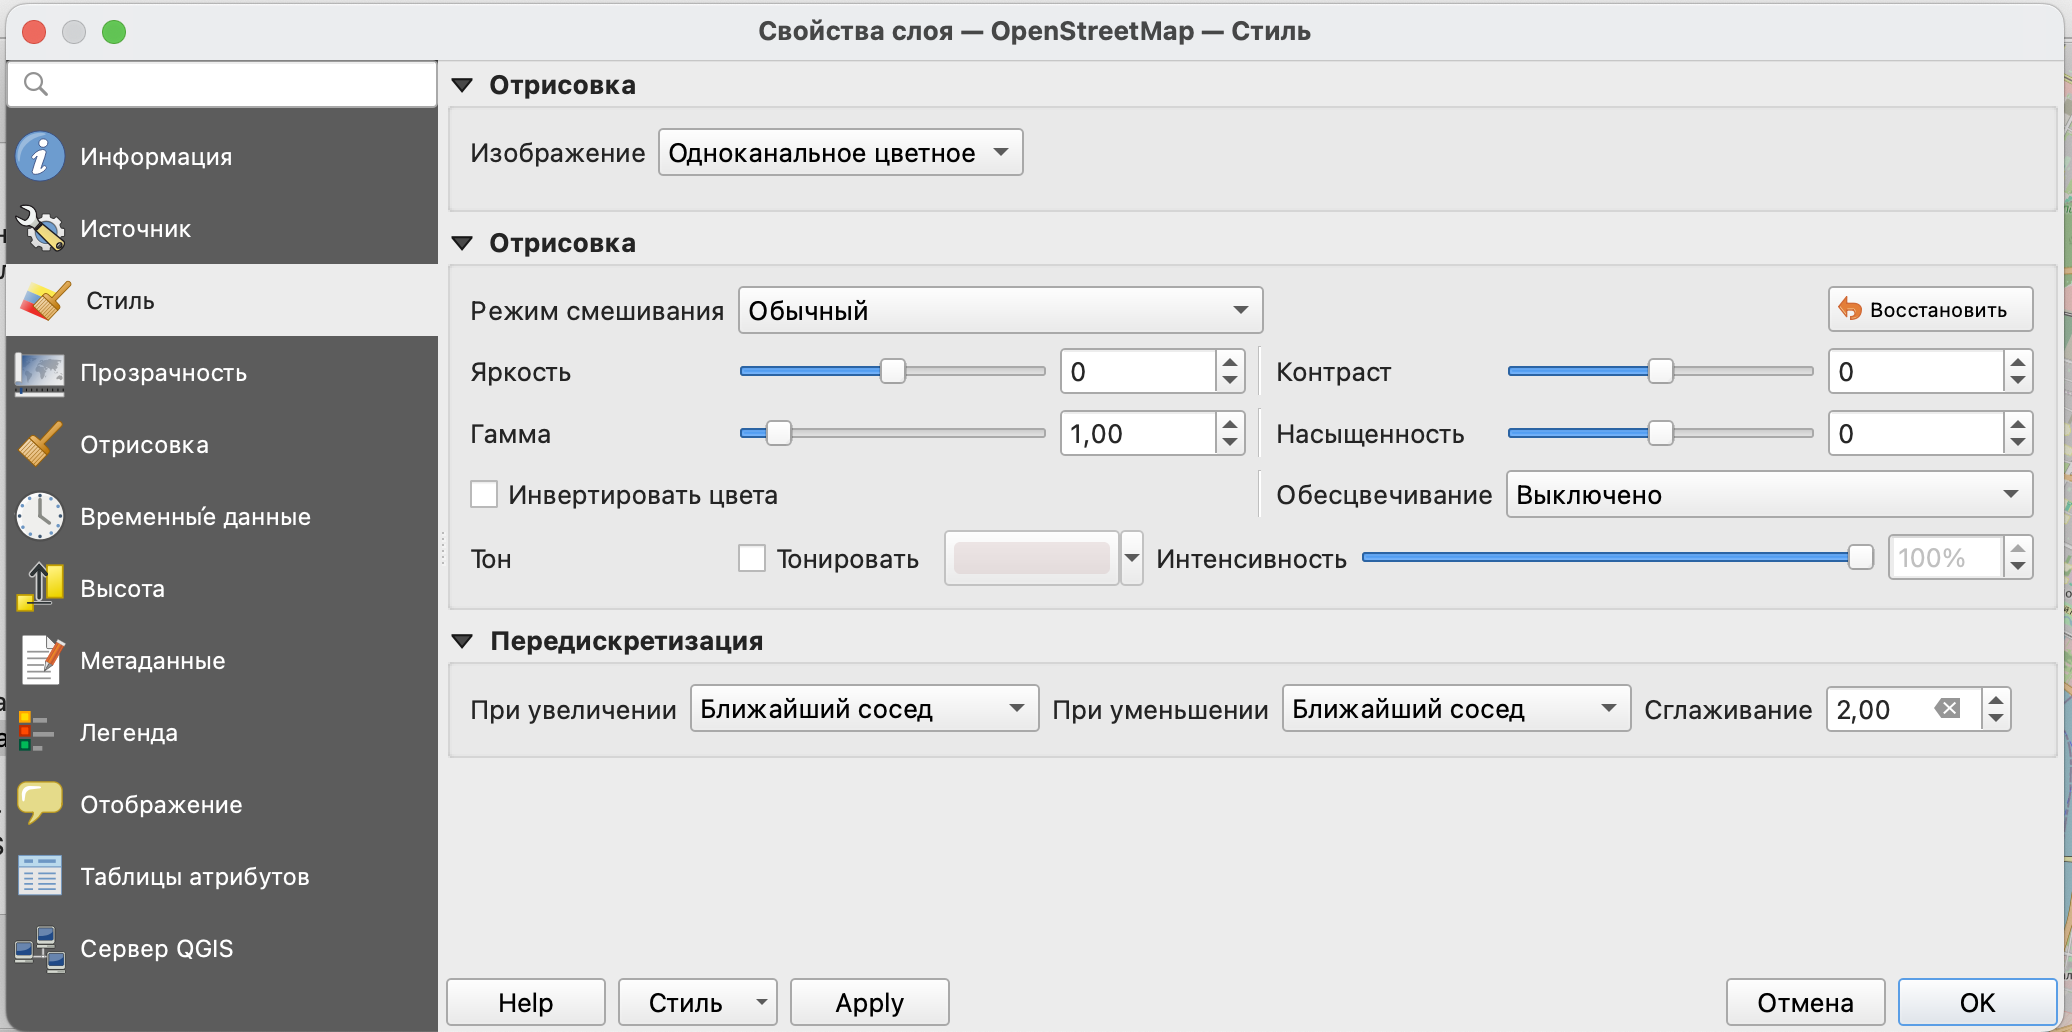
\includegraphics[width=18.82292in,height=\textheight,keepaspectratio]{images/clipboard-3430937073.png}
\end{center}

\subsubsection{Черно-белая
подложка}\label{ux447ux435ux440ux43dux43e-ux431ux435ux43bux430ux44f-ux43fux43eux434ux43bux43eux436ux43aux430}

Если вы хотите получить черно-белый вариант цветной подложки, то вы
можете снизить насыщенность до минимума.

\pandocbounded{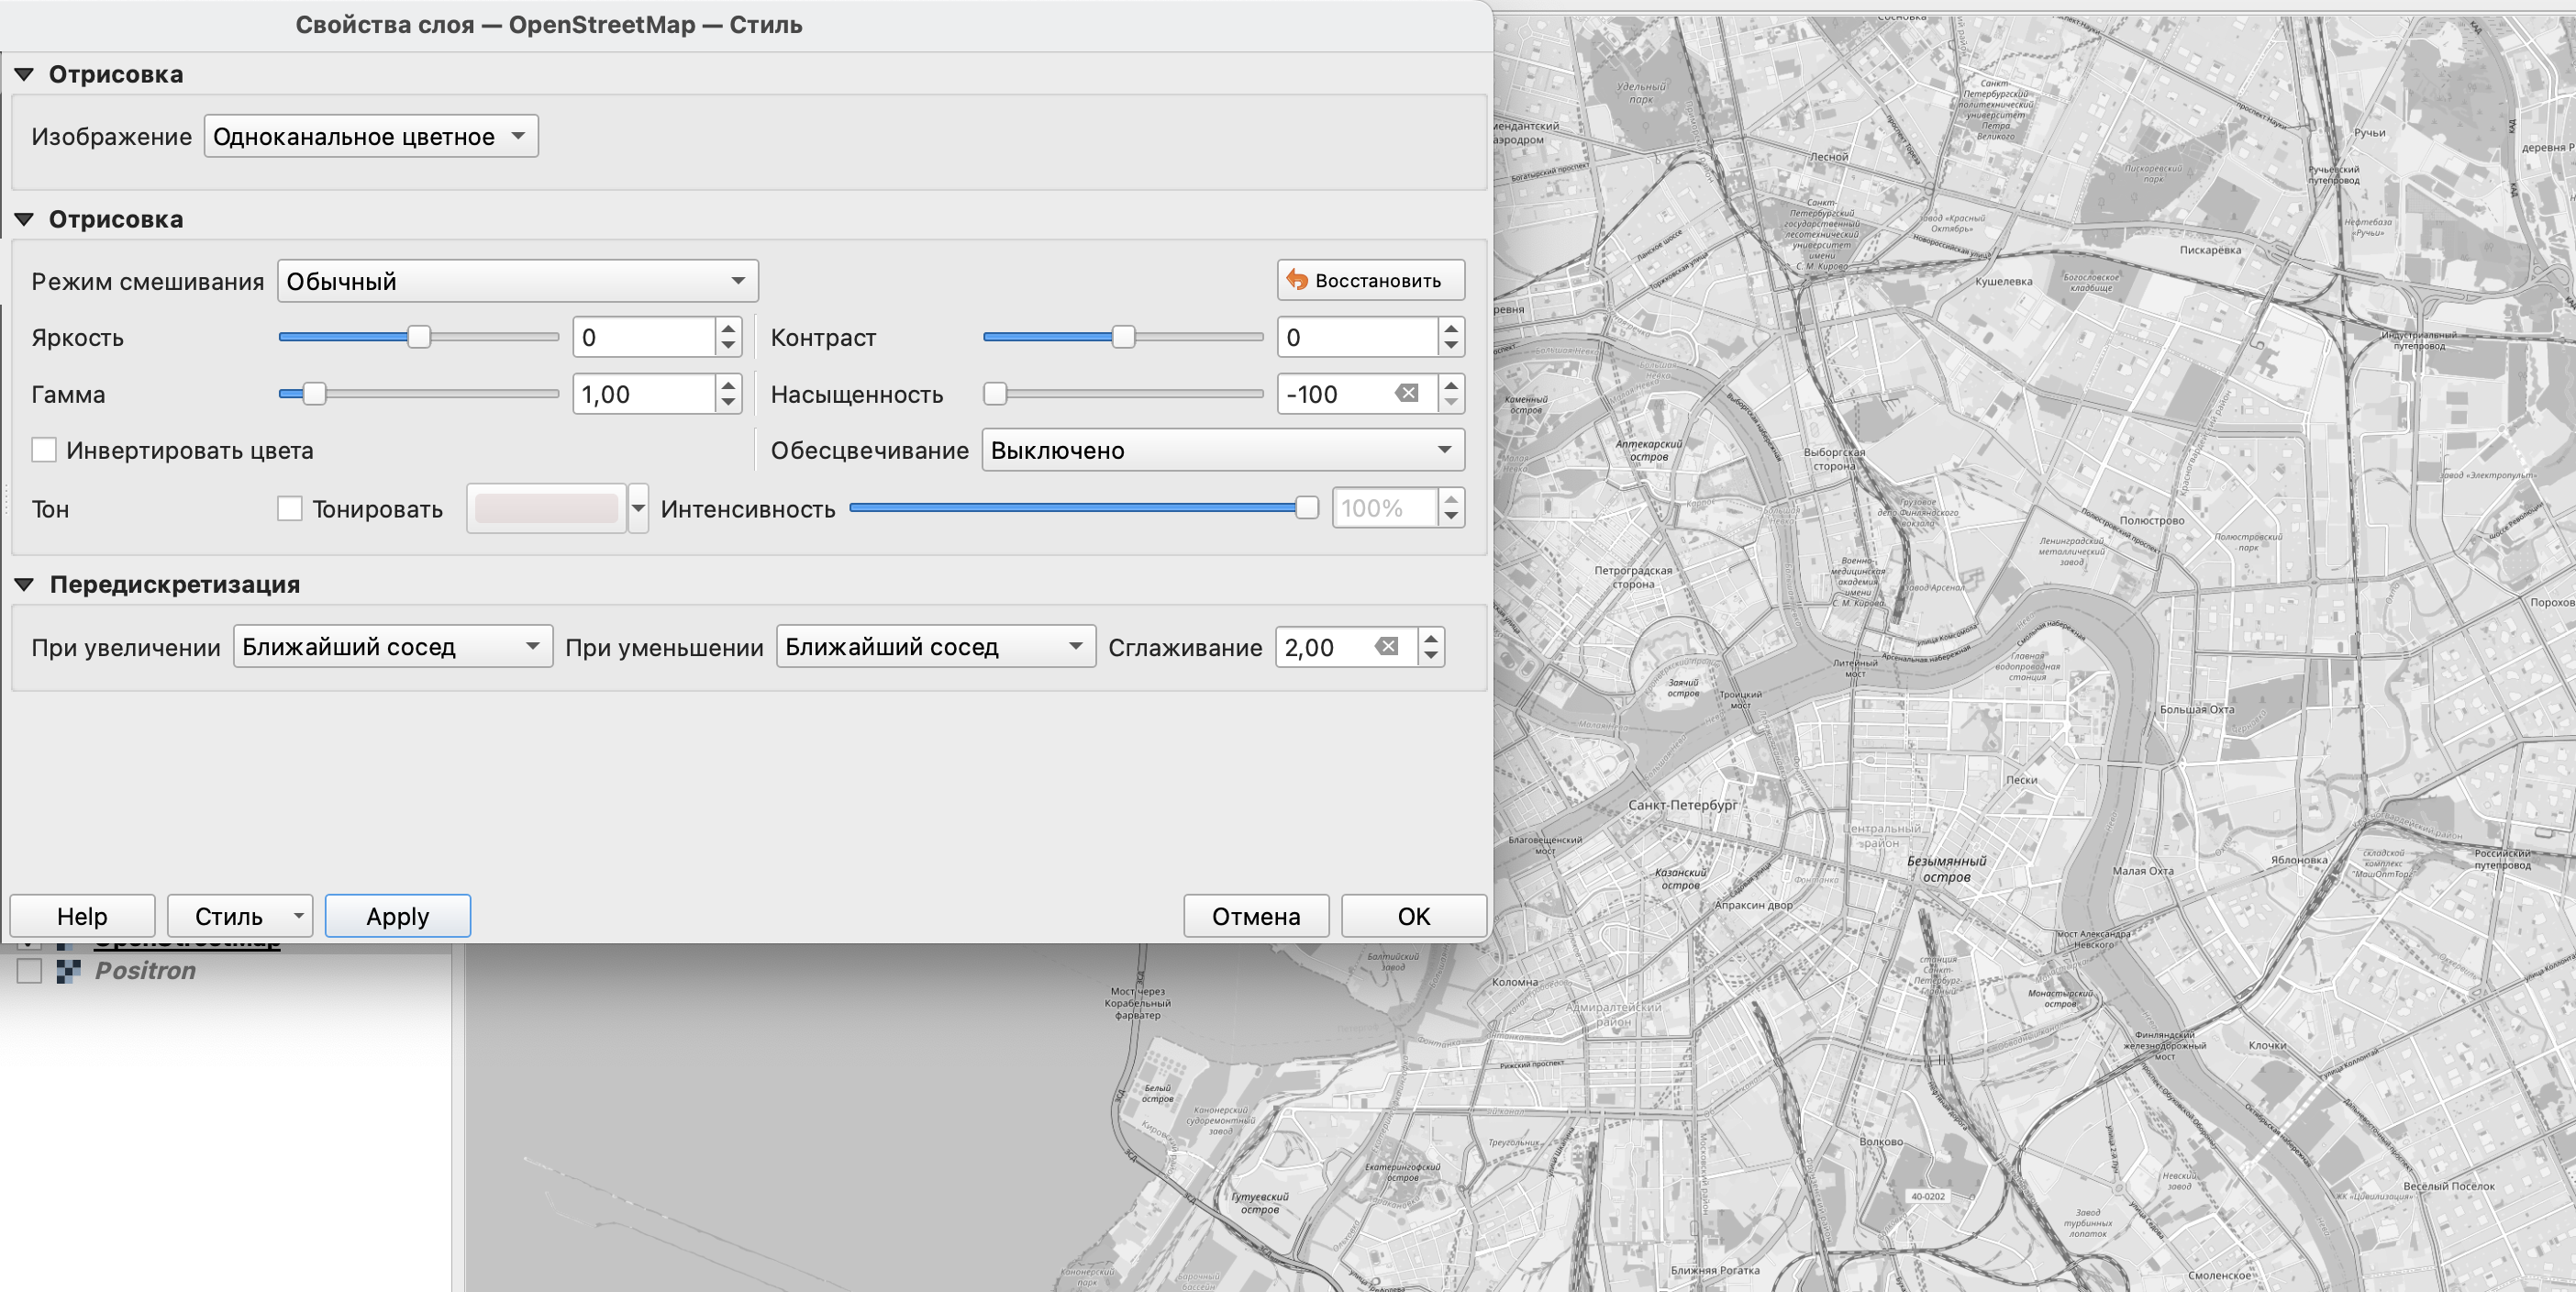
\includegraphics[keepaspectratio]{images/clipboard-3066223731.png}}

Вторым способом будет добавление обесцвечивания.

\pandocbounded{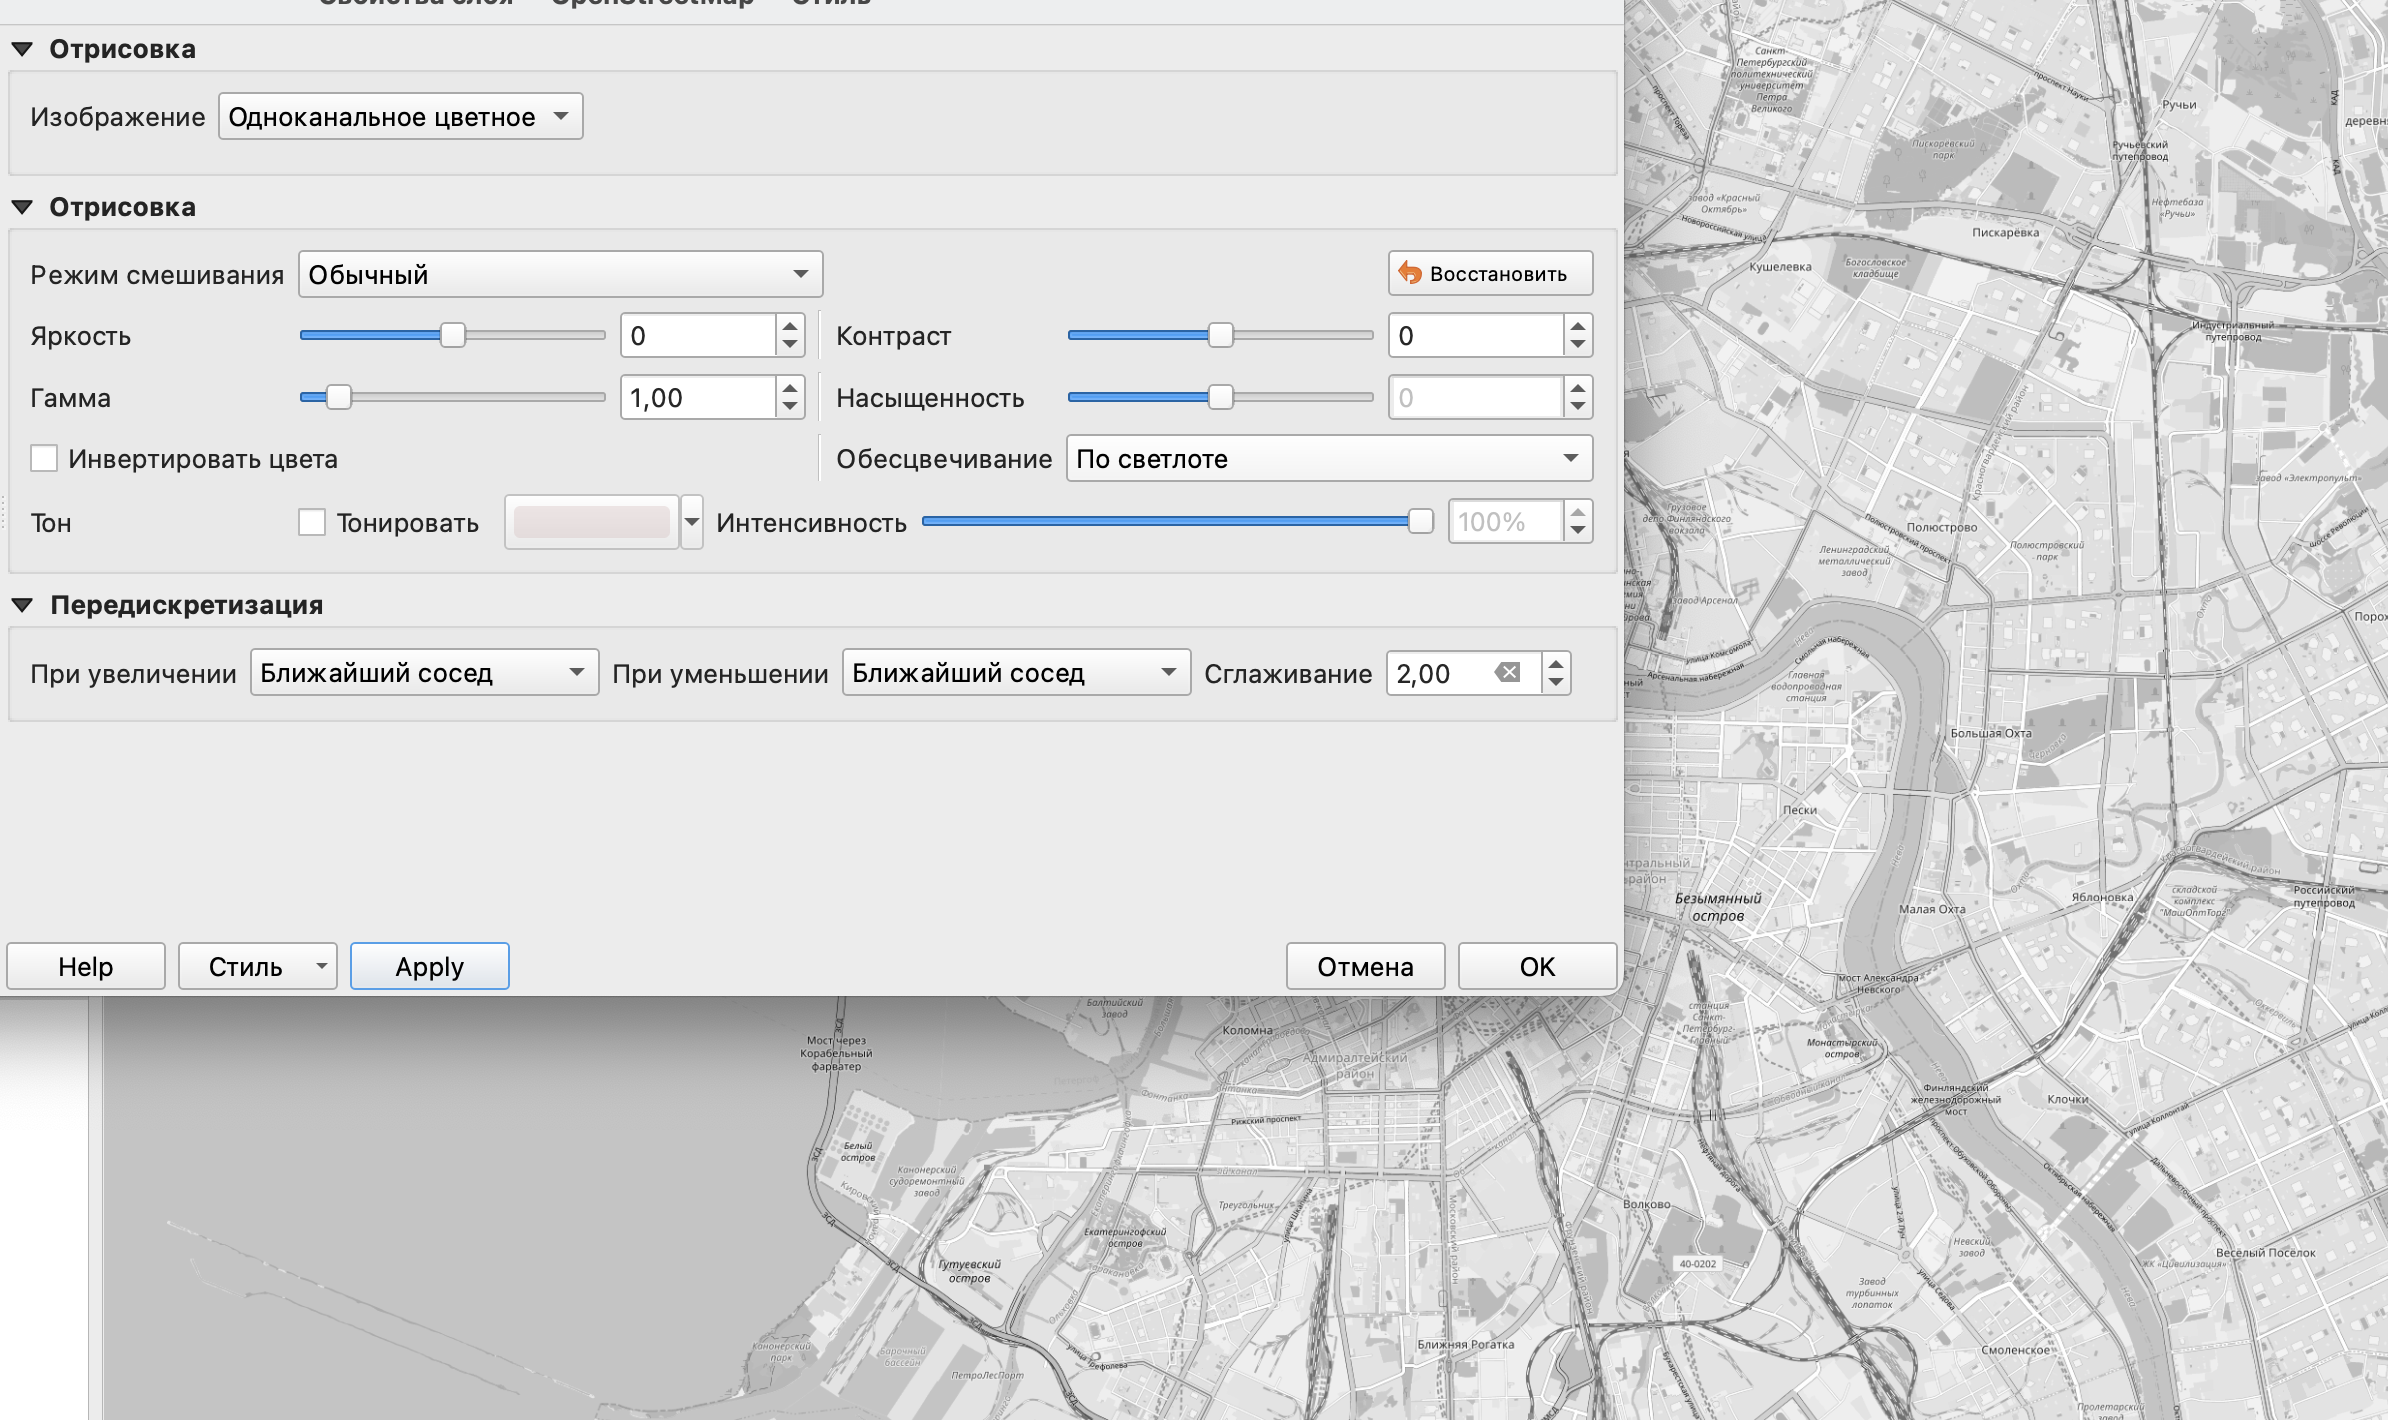
\includegraphics[keepaspectratio]{images/clipboard-3692804174.png}}

Если вы обесцветите изображение, а потом инвертируете, то вы получите
темный вариант подложки.

\pandocbounded{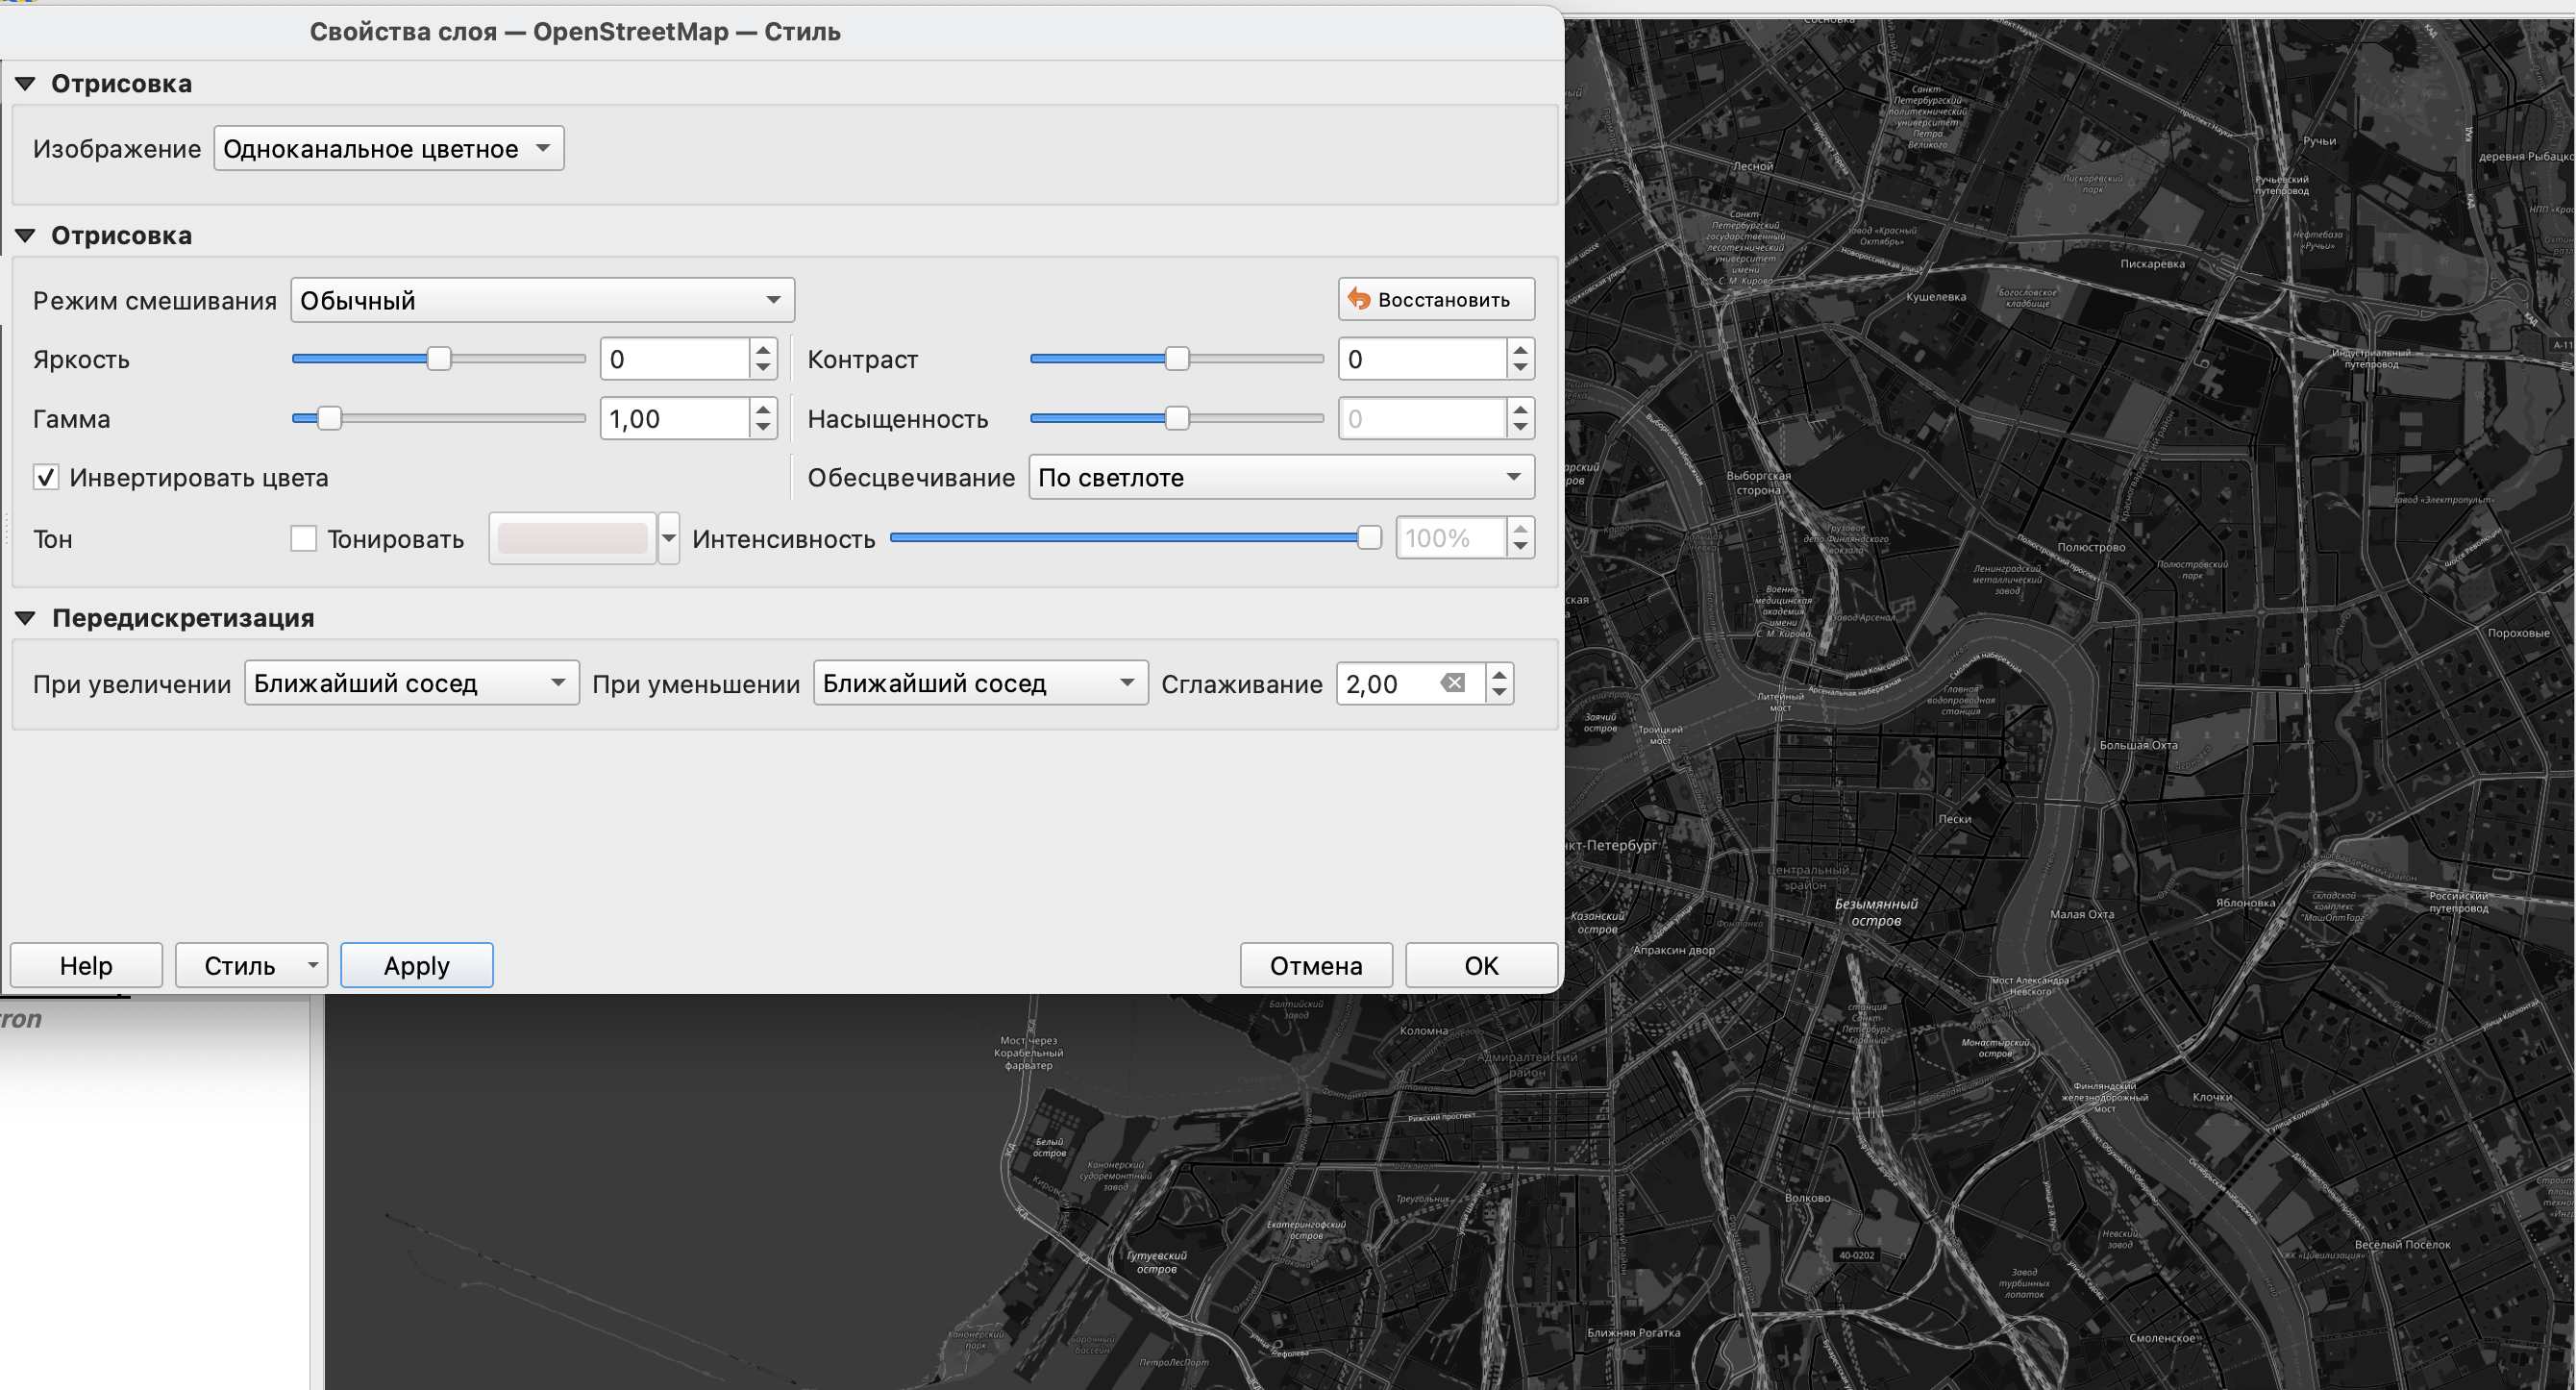
\includegraphics[keepaspectratio]{images/clipboard-1692698825.png}}

При использовании преимущественно монохромной подложки инвертирование
превратит светлую карту в темную и наоборот: темную в светлую.

\pandocbounded{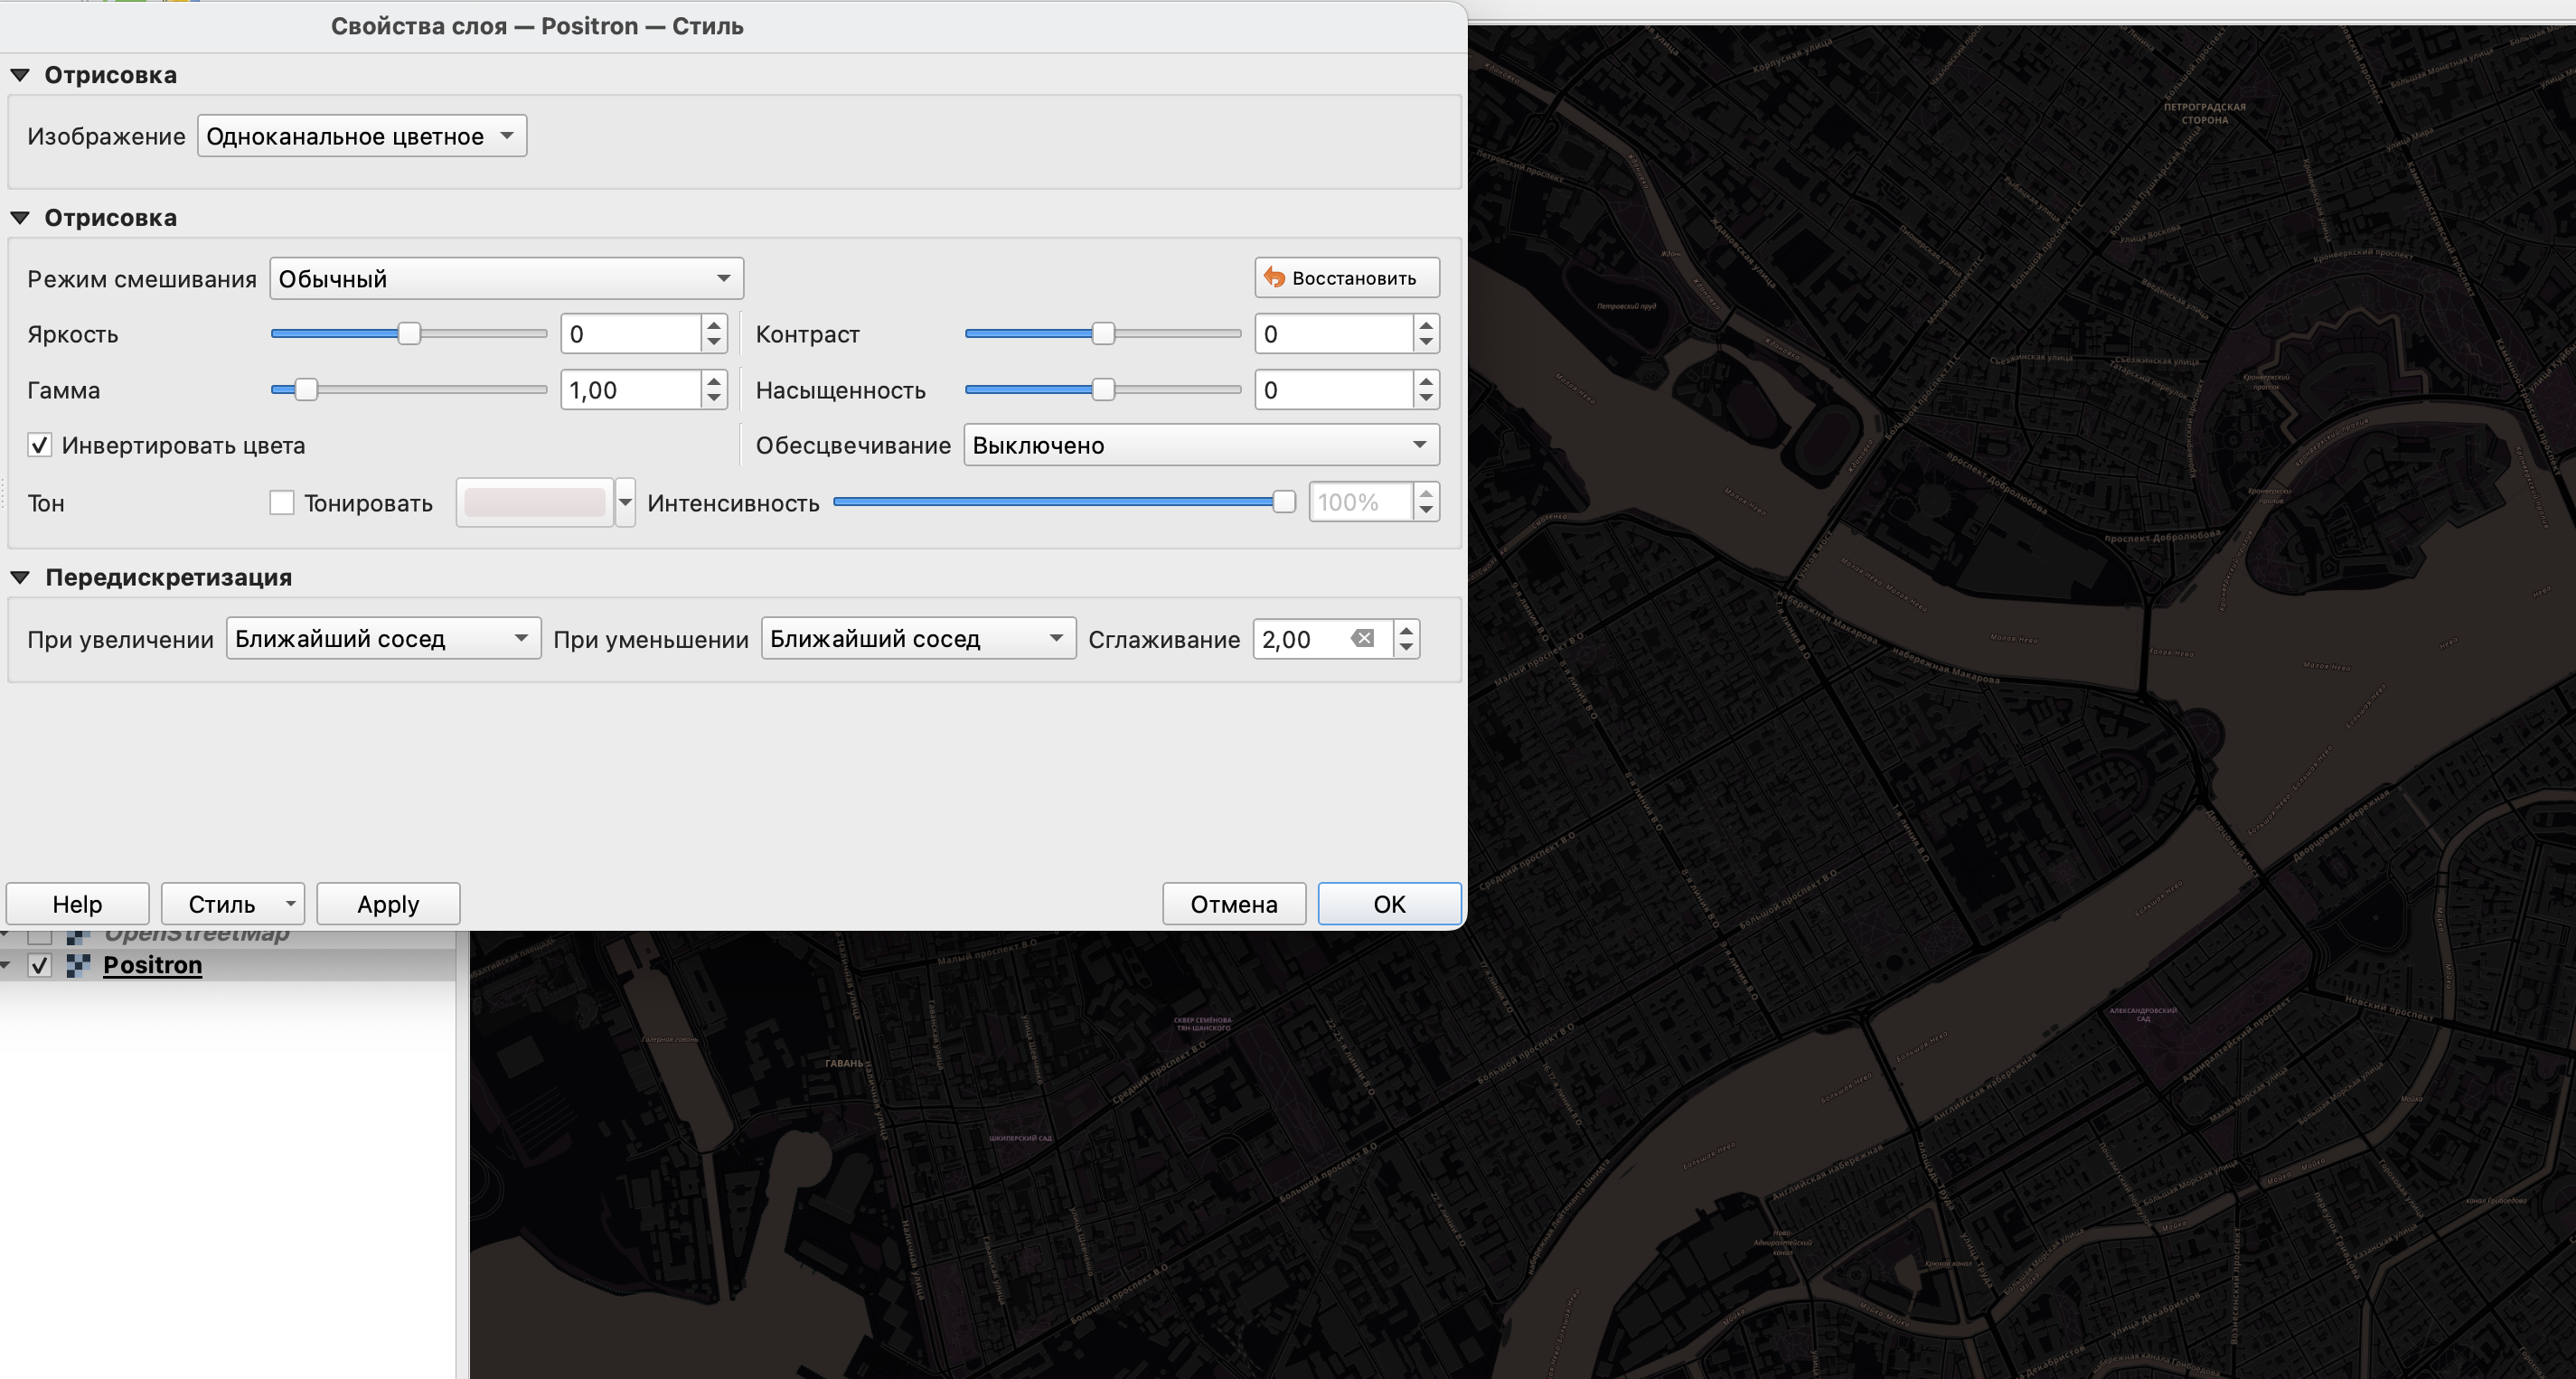
\includegraphics[keepaspectratio]{images/clipboard-1728003647.png}}

\subsubsection{Тонирование
карты}\label{ux442ux43eux43dux438ux440ux43eux432ux430ux43dux438ux435-ux43aux430ux440ux442ux44b}

Подложку как любое растровое изображение можно тонировать в тот оттенок,
который вы посчитаете нужным.

Для этого нужно поставить галочку слева от слова \emph{Тонировать} в
настройках стиля и выбрать нужный цвет. Настройка интенсивности здесь
позволяет выбрать степень тонирования.

\begin{center}
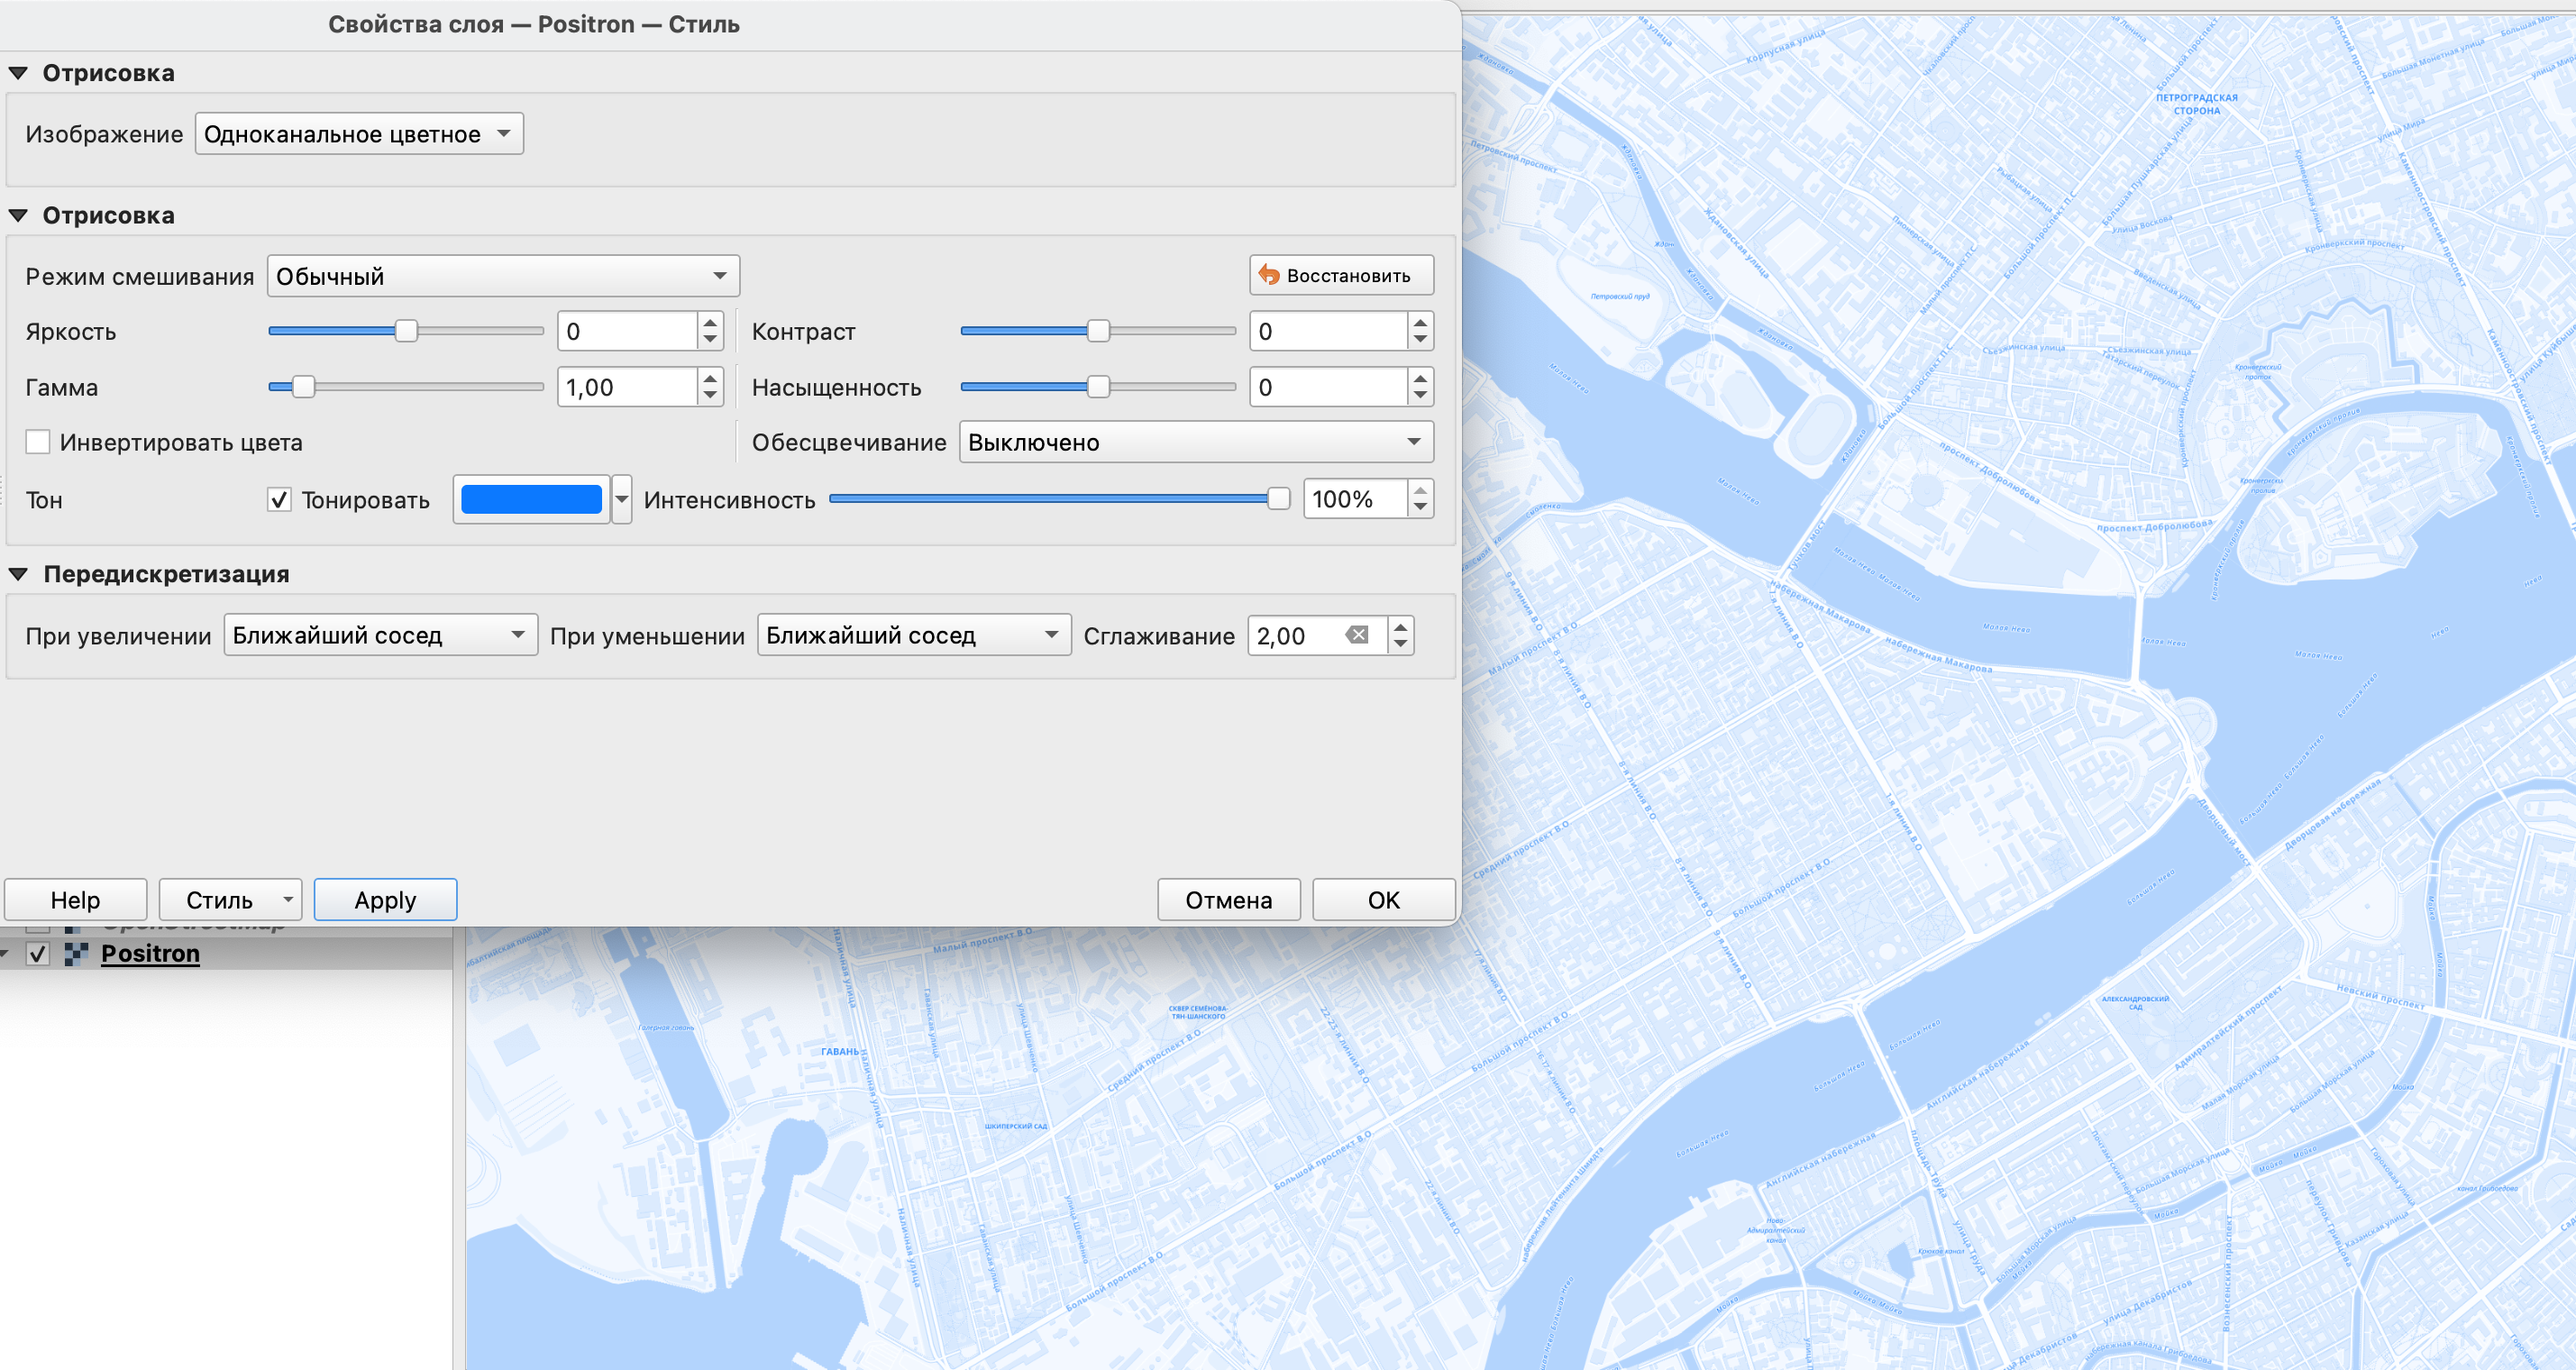
\includegraphics[width=19.58333in,height=\textheight,keepaspectratio]{images/clipboard-1921987371.png}
\end{center}

\begin{center}
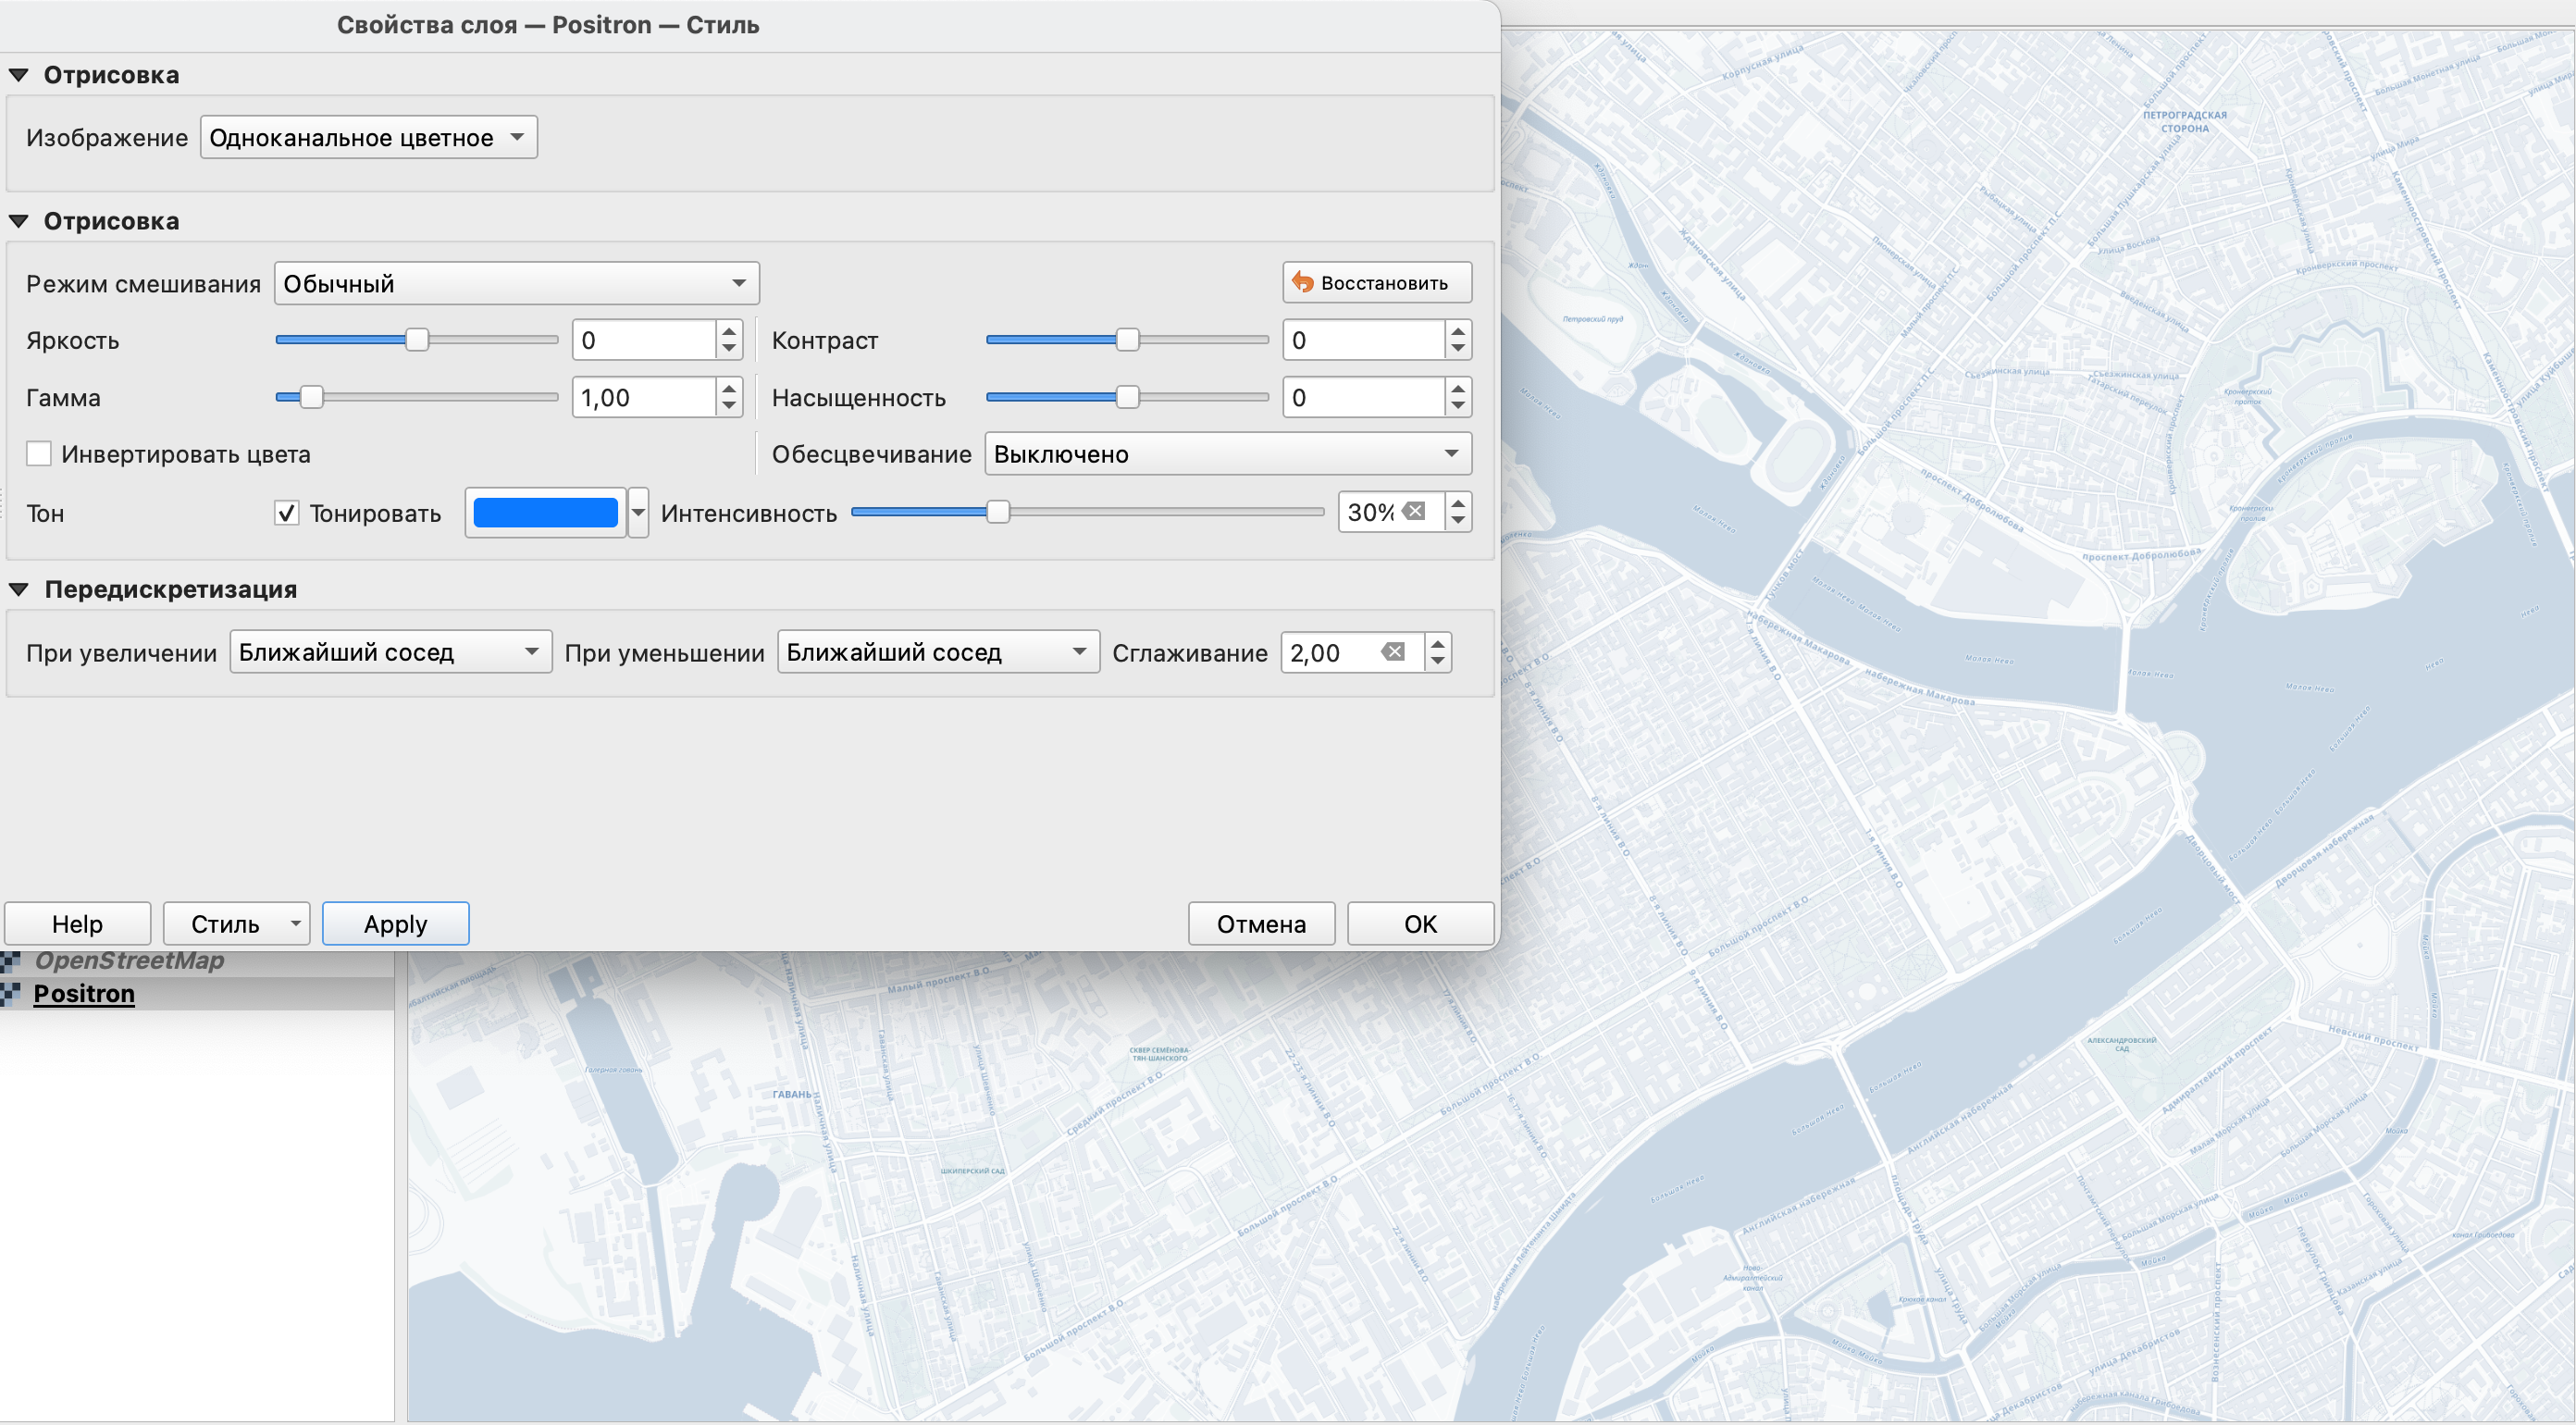
\includegraphics[width=18.83333in,height=\textheight,keepaspectratio]{images/clipboard-984317181.png}
\end{center}

Использование одновременно нескольких настроек позволяет добиться
дополнительного художественного эффекта.

\pandocbounded{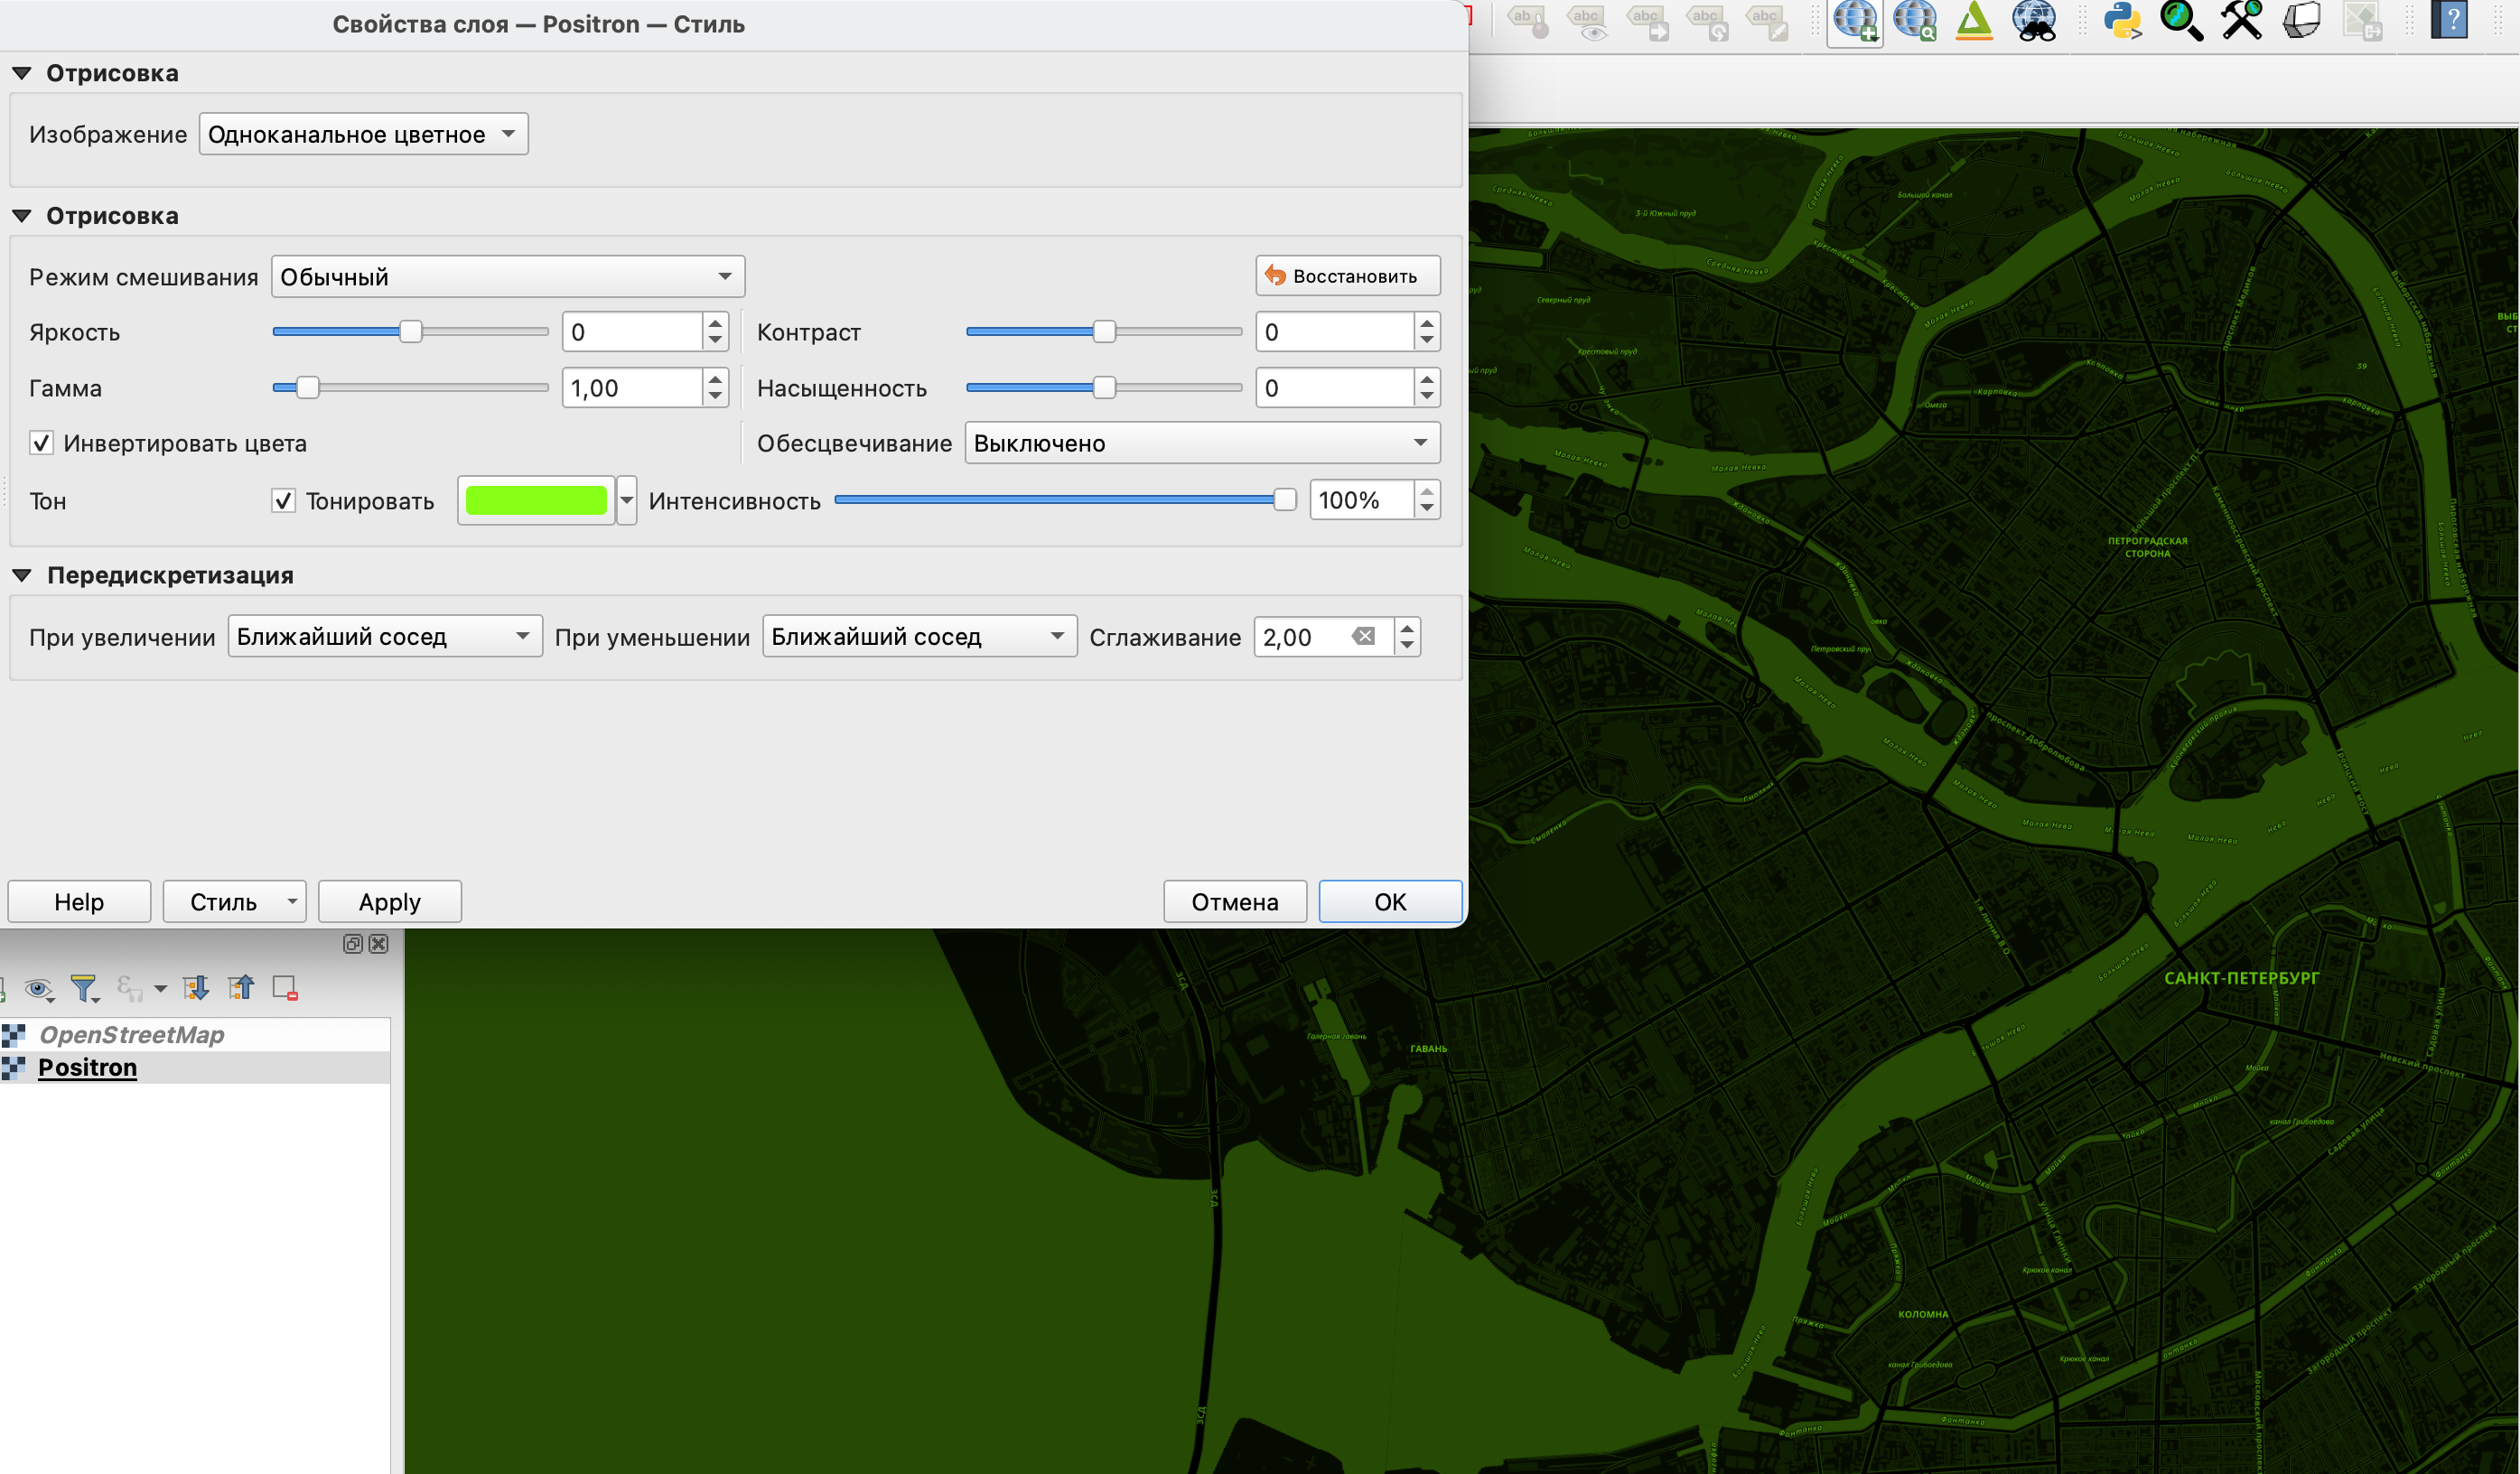
\includegraphics[keepaspectratio]{images/clipboard-2465586496.png}}

\section{Работа с векторными
слоями}\label{ux440ux430ux431ux43eux442ux430-ux441-ux432ux435ux43aux442ux43eux440ux43dux44bux43cux438-ux441ux43bux43eux44fux43cux438}

\subsection{Создание
слоя}\label{ux441ux43eux437ux434ux430ux43dux438ux435-ux441ux43bux43eux44f}

Новый векторный слой можно создать из панели инструментов (кнопка
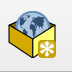
\includegraphics[width=0.40625in,height=\textheight,keepaspectratio]{images/clipboard-4258986521.png}
\emph{Создать слой GeoPackage}) или из строки меню: \emph{Слой}
\(\longrightarrow\) Создать слой.

\begin{center}
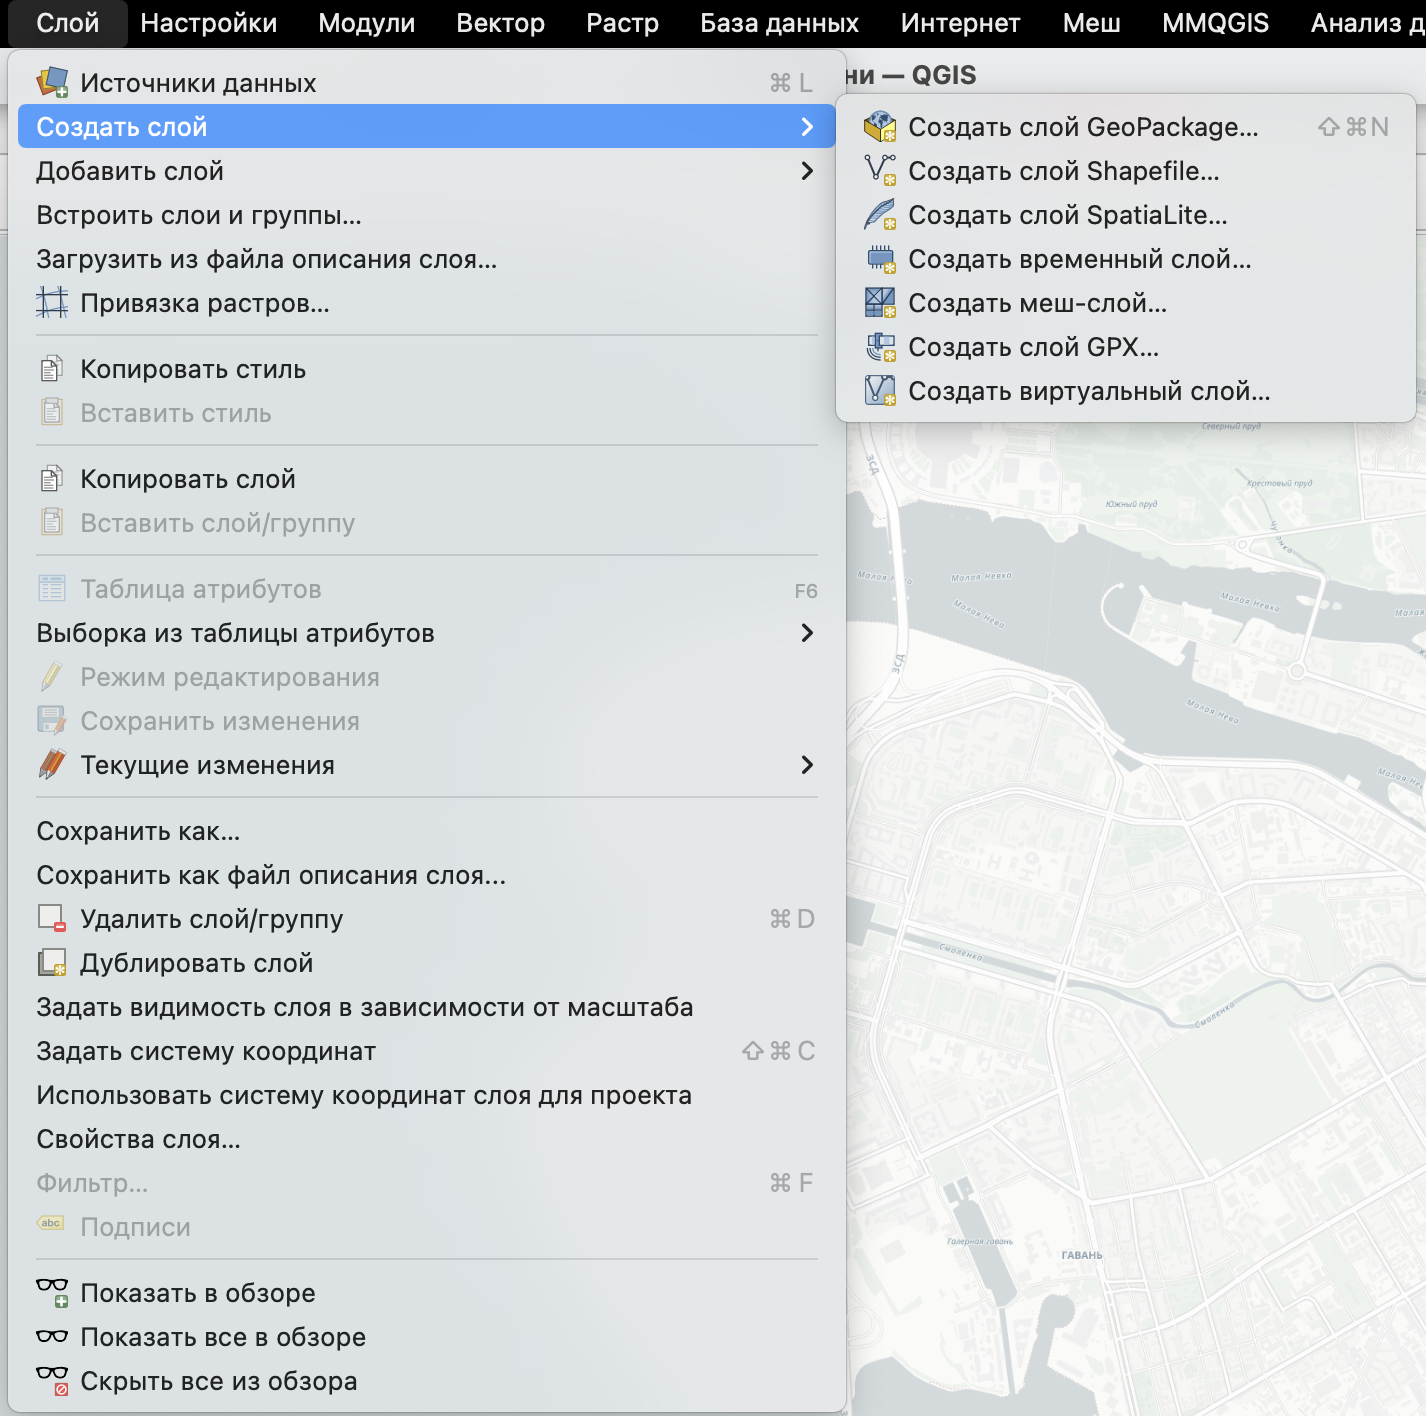
\includegraphics[width=9.4375in,height=\textheight,keepaspectratio]{images/clipboard-4193668470.png}
\end{center}

\begin{tcolorbox}[enhanced jigsaw, arc=.35mm, bottomrule=.15mm, bottomtitle=1mm, breakable, colback=white, colbacktitle=quarto-callout-important-color!10!white, colframe=quarto-callout-important-color-frame, coltitle=black, left=2mm, leftrule=.75mm, opacityback=0, opacitybacktitle=0.6, rightrule=.15mm, title=\textcolor{quarto-callout-important-color}{\faExclamation}\hspace{0.5em}{Важно}, titlerule=0mm, toprule=.15mm, toptitle=1mm]

На этом этапе вам сразу нужно выбрать тип файла, который вы будете
создавать. Рекомендую выбирать формат GeoPackage.

\end{tcolorbox}

Далее необходимо выбрать куда и под каким именем вы будете сохранять
свой файл. Так как у меня на картинке показан именно GeoPackage, то
вместо слов \emph{Имя файла} указано \emph{База данных}.

\begin{tcolorbox}[enhanced jigsaw, arc=.35mm, bottomrule=.15mm, bottomtitle=1mm, breakable, colback=white, colbacktitle=quarto-callout-caution-color!10!white, colframe=quarto-callout-caution-color-frame, coltitle=black, left=2mm, leftrule=.75mm, opacityback=0, opacitybacktitle=0.6, rightrule=.15mm, title=\textcolor{quarto-callout-caution-color}{\faFire}\hspace{0.5em}{Предупреждение}, titlerule=0mm, toprule=.15mm, toptitle=1mm]

В пункте \emph{База данных} (или \emph{Имя файла}) недостаточно указать
просто имя файла, там должен быть отображен полный путь к файлу, поэтому
необходимо нажать кнопку обзора
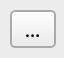
\includegraphics[width=0.40625in,height=0.375in]{images/clipboard-3642390843.png},
выбрать папку для сохранения и задать имя файла.

\end{tcolorbox}

\begin{center}
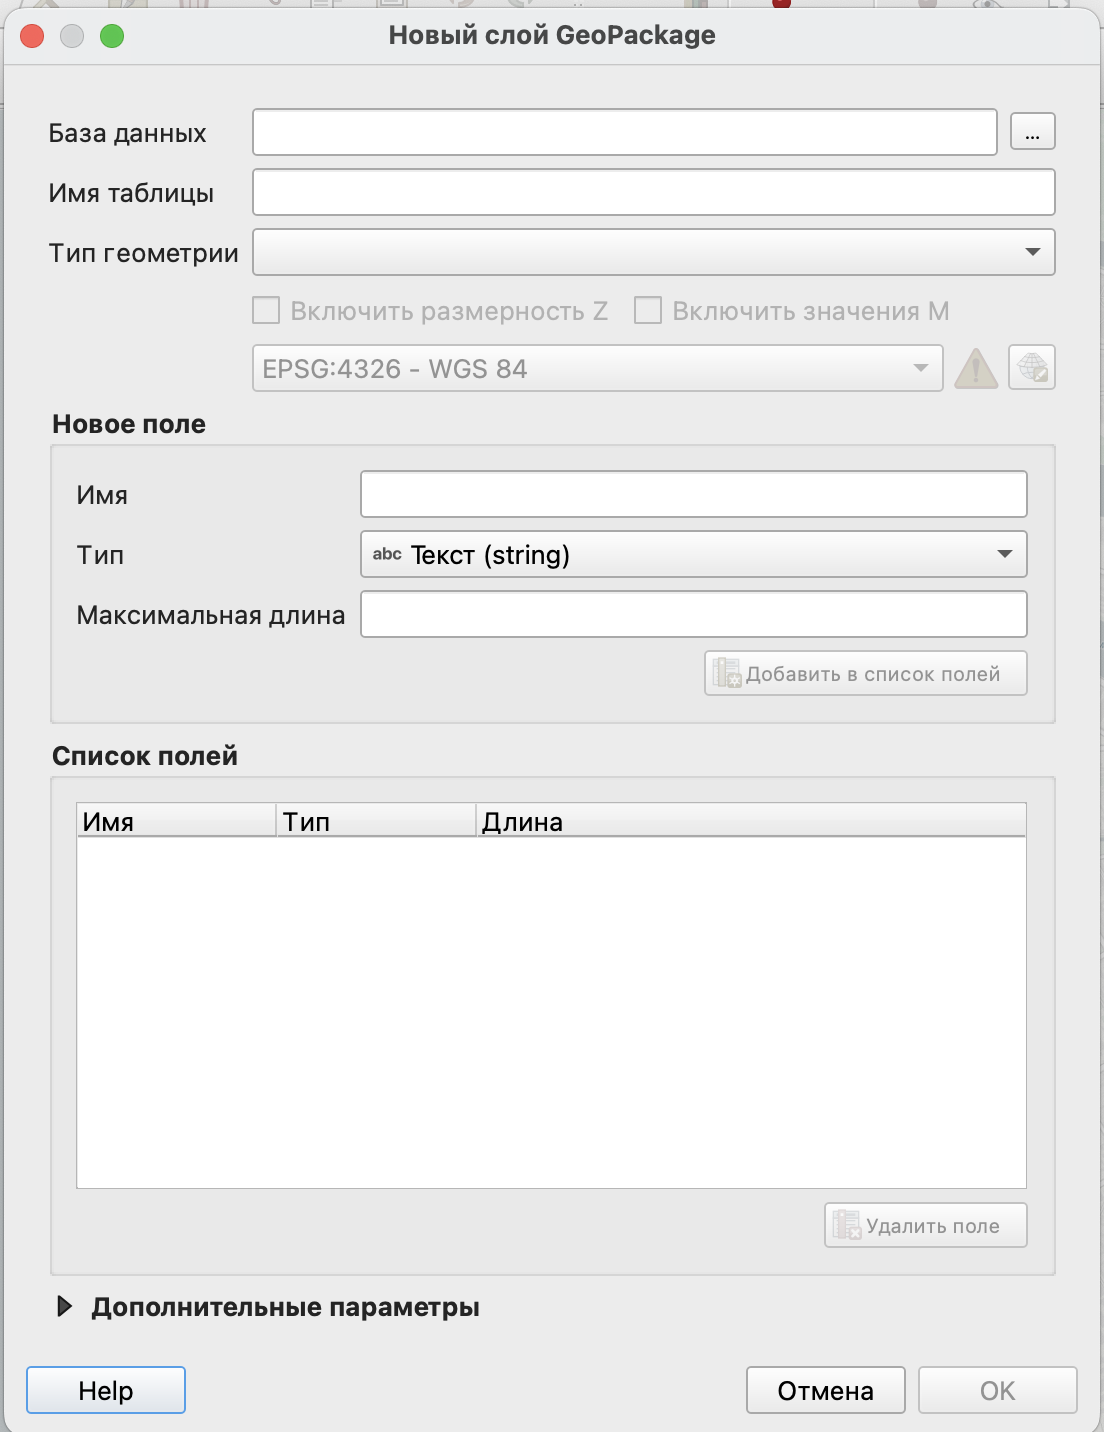
\includegraphics[width=6.42708in,height=\textheight,keepaspectratio]{images/clipboard-979152897.png}
\end{center}

\emph{Имя таблицы}, как правило, соответствует имени файла.

Тип геометрии вы для создания примера можете выбрать любой, в моем
случае будут рассмотрены полигоны, так как они дают больше всего
возможностей для редактирования.

По типом геометрии вам предлагают выбрать систему координат для слоя,
предлагая одну из них по умолчанию. О системах координат мы поговорим
чуть позднее, поэтому пока оставим предложенный нам вариант.

Ниже под заголовком \textbf{Новое поле} вы можете создать структуру
своей атрибутивной таблицы, то есть какие столбцы с какими названиями и
типами данных в ней будут. Для этого нужно указать имя столбца и тип
данных.

\begin{tcolorbox}[enhanced jigsaw, arc=.35mm, bottomrule=.15mm, bottomtitle=1mm, breakable, colback=white, colbacktitle=quarto-callout-important-color!10!white, colframe=quarto-callout-important-color-frame, coltitle=black, left=2mm, leftrule=.75mm, opacityback=0, opacitybacktitle=0.6, rightrule=.15mm, title=\textcolor{quarto-callout-important-color}{\faExclamation}\hspace{0.5em}{Важно}, titlerule=0mm, toprule=.15mm, toptitle=1mm]

Имена столбцов обязательно должны быть уникальными.

\end{tcolorbox}

Если на этом этапе вы ошибетесь в списке полей или вообще ничего не
укажете, то это не страшно, так как потом вы можете отредактировать это
средствами работы с таблицей атрибутов.

Для того, чтобы столбец был добавлен в таблицу атрибутов, нужно нажать
кнопку \emph{Добавить в список полей}, после чего он будет отображен в
списке ниже.

Очень рекомендую впоследствии стараться давать осмысленные имена своим
слоям и файлам, чтобы вы могли без проблем вспомнить, что в них
хранится.

После создания слой появится в вашей панели слоев. Обратите внимание,
что слева от названия слоя будет показана точка для слоя с точечными
объектами, линия - для слоя с линейными объектами и квадрат - для слоя с
полигональными объектами.

При этом изображение на карте у вас не поменялось, так как пока у вас не
было добавлено никаких объектов в слой.

\begin{tcolorbox}[enhanced jigsaw, arc=.35mm, bottomrule=.15mm, bottomtitle=1mm, breakable, colback=white, colbacktitle=quarto-callout-important-color!10!white, colframe=quarto-callout-important-color-frame, coltitle=black, left=2mm, leftrule=.75mm, opacityback=0, opacitybacktitle=0.6, rightrule=.15mm, title=\textcolor{quarto-callout-important-color}{\faExclamation}\hspace{0.5em}{Важно}, titlerule=0mm, toprule=.15mm, toptitle=1mm]

Обратите внимание, что при клике на название слоя, оно подсвечивается,
таким образом показывается \textbf{активный слой}. Все действия,
выполняемые в программе происходят с активным слоем.

\end{tcolorbox}

\subsection{Создание и редактирование
объектов}\label{ux441ux43eux437ux434ux430ux43dux438ux435-ux438-ux440ux435ux434ux430ux43aux442ux438ux440ux43eux432ux430ux43dux438ux435-ux43eux431ux44aux435ux43aux442ux43eux432}

Для того, чтобы начать создание объектов, слой необходимо сделать
редактируемым. Это осуществляется либо путем нажатия на кнопку
\emph{Начать редактирование}

\includegraphics[width=0.42708in,height=\textheight,keepaspectratio]{images/clipboard-3707174716.png},
либо из контекстного меню слоя.

\begin{center}
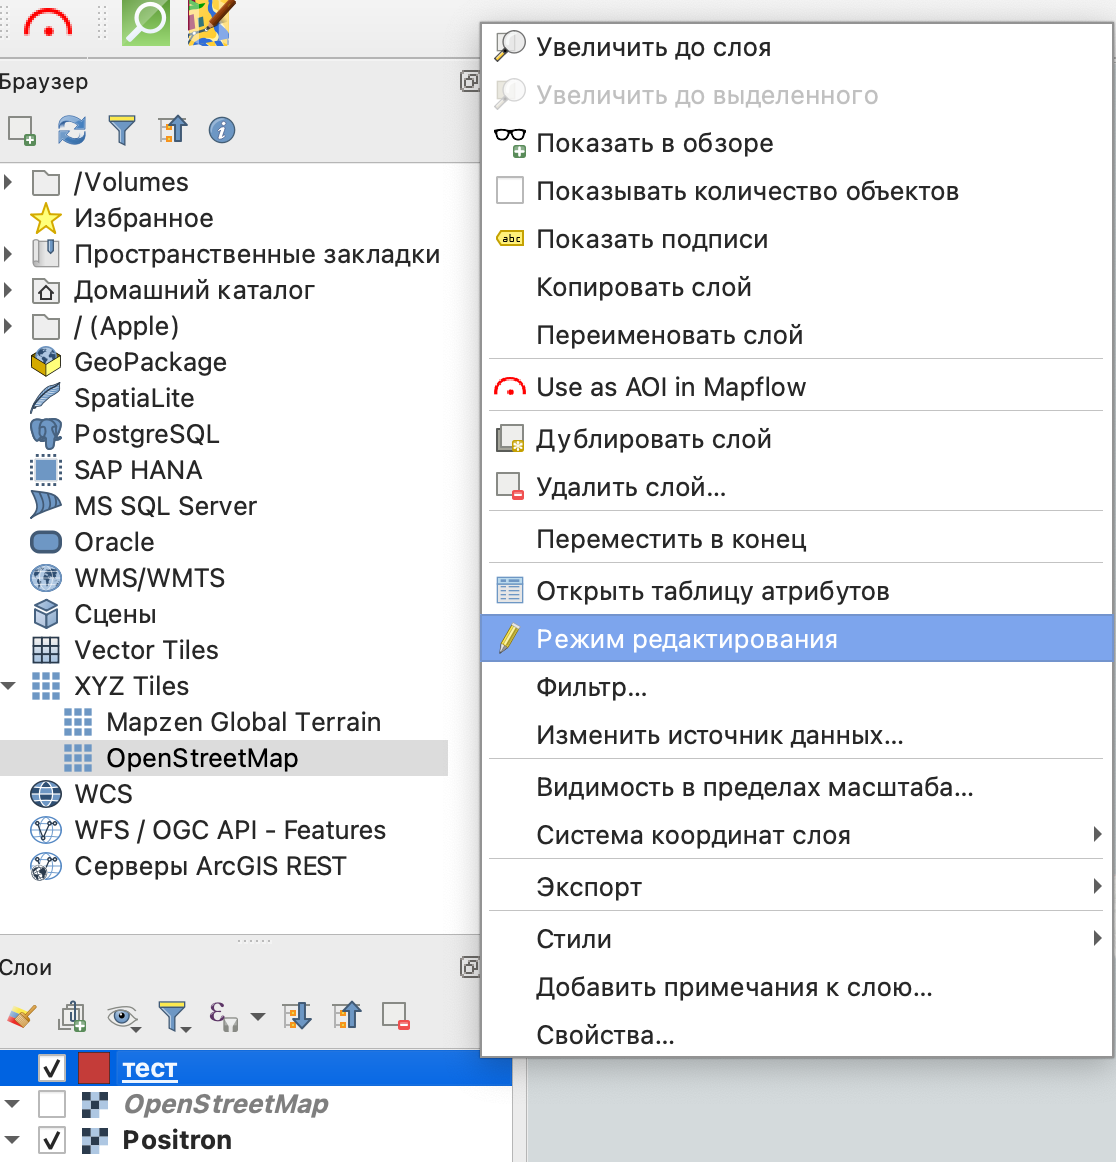
\includegraphics[width=7in,height=\textheight,keepaspectratio]{images/clipboard-3592244129.png}
\end{center}

После того, как слой стал перешел в режим редактирования слева от его
имени появится знак карандаша, символизирующий этот статус, а основная
панель инструментов изменится и на ней активируются инструменты создания
и редактирования векторных объектов.

По умолчанию создание объекта здесь выполняется сегментами, то есть
отрезками прямых линий между поворотными точками. Каждая поворотная
точка указывается кликом левой кнопки мыши, а завершение отрисовки
происходит по клику правой кнопки.

Отметить отрисовку объекта можно просто нажав в процессе кнопку
\emph{Escape} на клавиатуре.

Создание точечных объектов происходит по клику, а линейные создаются
похоже на полигональные, только по завершении отрисовки не дополняются
до замкнутого контура.

Другие доступные опции кроме оцифровки сегментами:

\begin{center}
\pandocbounded{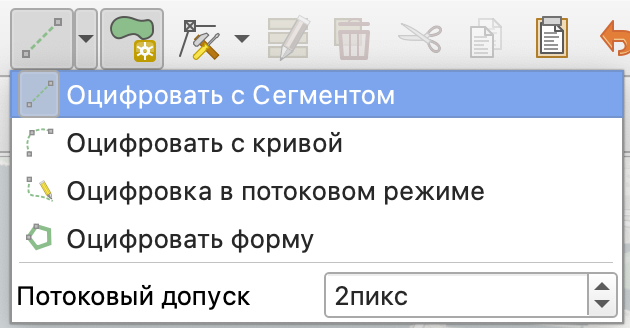
\includegraphics[keepaspectratio]{images/clipboard-2449145075.png}}
\end{center}

\begin{itemize}
\tightlist
\item
  оцифровать с кривой
\end{itemize}

\begin{itemize}
\tightlist
\item
  оцифровка в потоковом режиме
\end{itemize}

\begin{itemize}
\tightlist
\item
  оцифровать форму
\end{itemize}

\begin{tcolorbox}[enhanced jigsaw, arc=.35mm, bottomrule=.15mm, bottomtitle=1mm, breakable, colback=white, colbacktitle=quarto-callout-tip-color!10!white, colframe=quarto-callout-tip-color-frame, coltitle=black, left=2mm, leftrule=.75mm, opacityback=0, opacitybacktitle=0.6, rightrule=.15mm, title=\textcolor{quarto-callout-tip-color}{\faLightbulb}\hspace{0.5em}{Дополнительно}, titlerule=0mm, toprule=.15mm, toptitle=1mm]

По умолчанию у вас после создания каждого объекта будет всплывать окно
заполнения атрибутов. Вы можете заполнять атрибуты сразу для каждого
объекта или потом сразу для всех в атрибутивной таблице. Главное, не
забывайте в этой форме нажимать OK, иначе объекты не будут созданы.

Если вы хотите отключить автоматическую форму, это можно сделать в
настройках программы: \emph{Настройки} \(\longrightarrow\)
\emph{Параметры}.

\pandocbounded{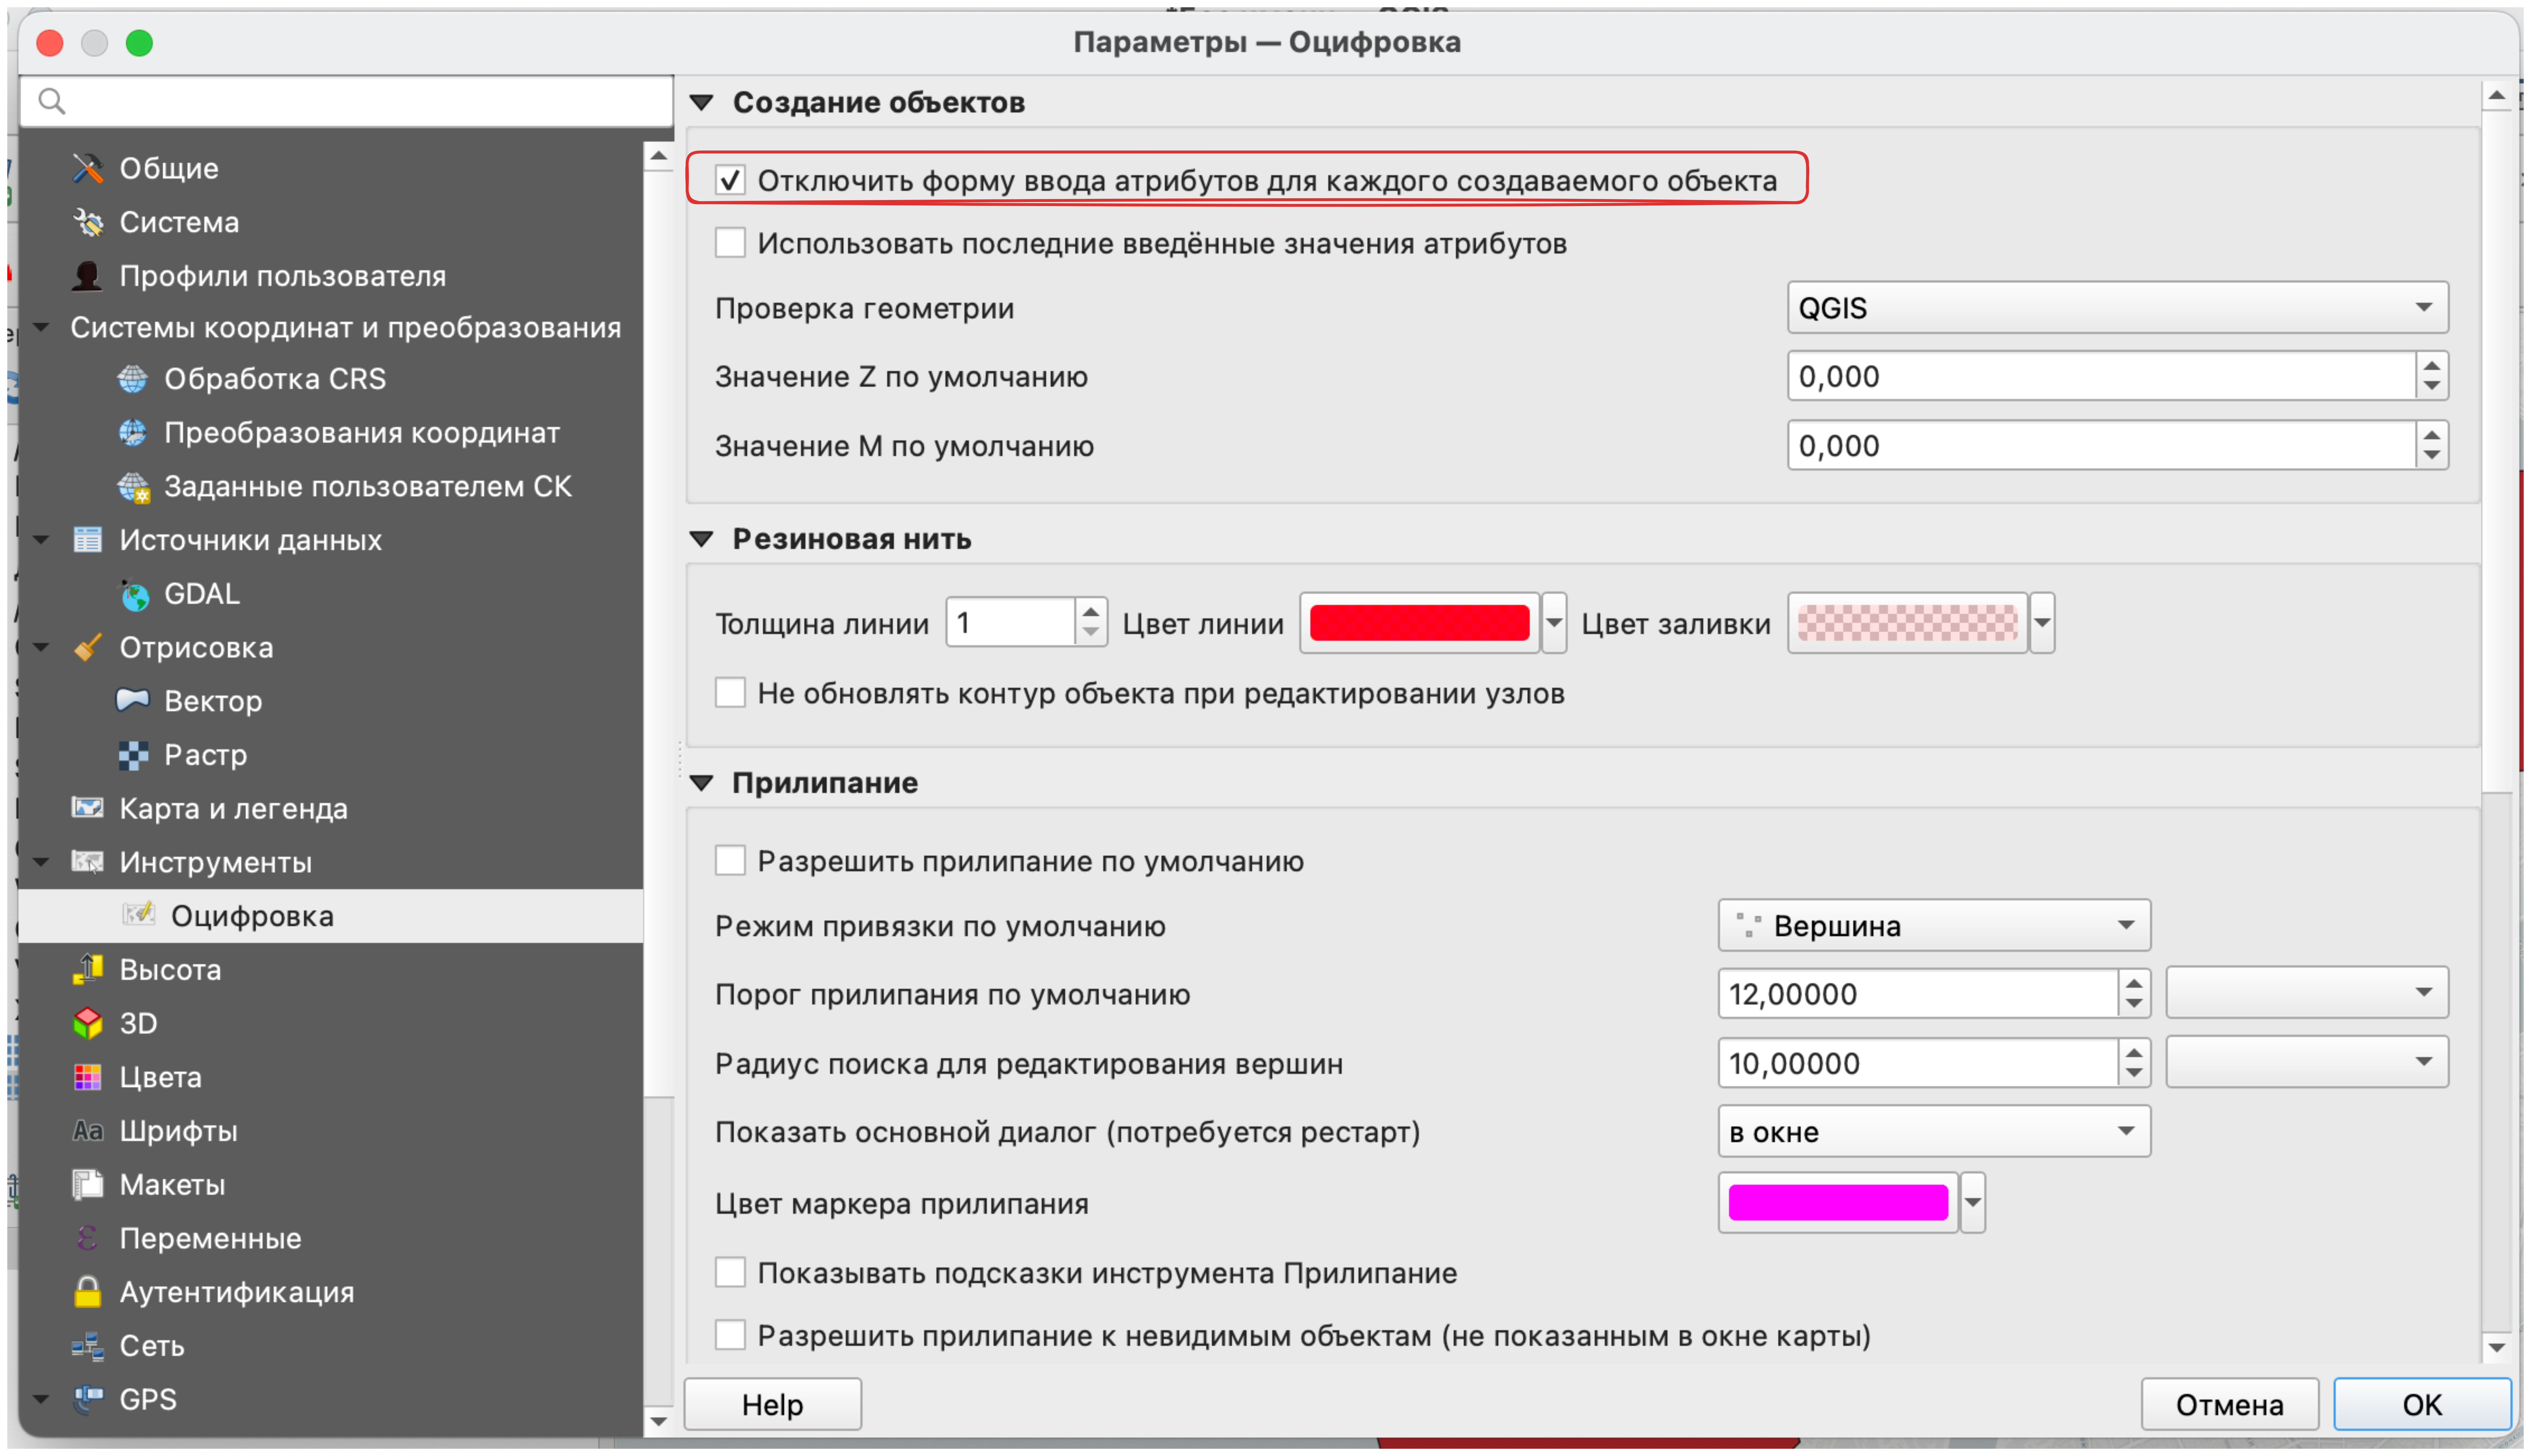
\includegraphics[keepaspectratio]{images/clipboard-3860238208.png}}

\end{tcolorbox}

В том случае, если вы хотите создавать объекты конкретной геометрической
формы (квадраты, круги, эллипсы), вы можете включить \emph{Панель
инструментов оцифровки}.

\begin{center}
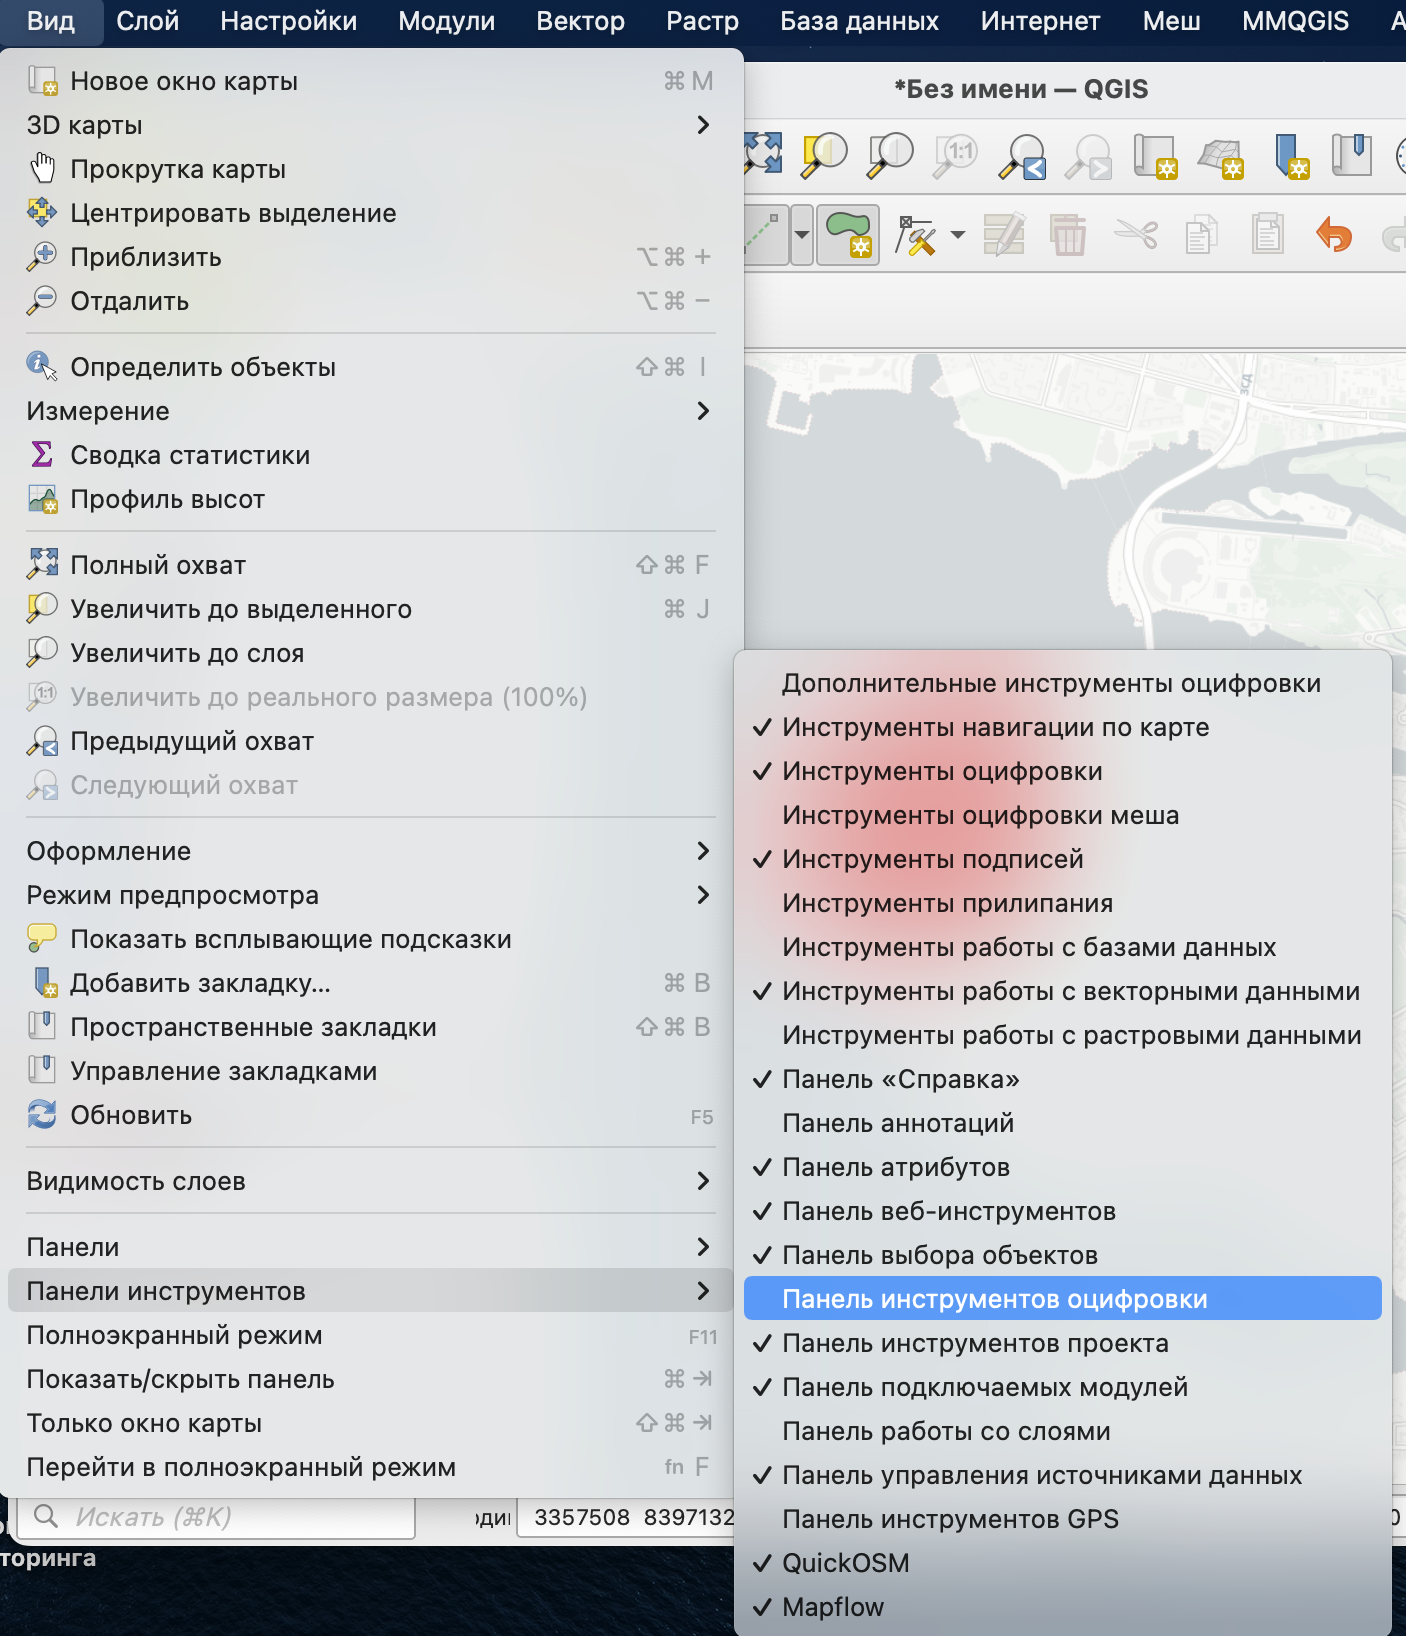
\includegraphics[width=8.05208in,height=\textheight,keepaspectratio]{images/clipboard-755946127.png}
\end{center}

Эта панель будет добавлена на панель инструментов и позволит вам
создавать геометрические объекты определенной формы с различными
параметрами:

\begin{center}
\pandocbounded{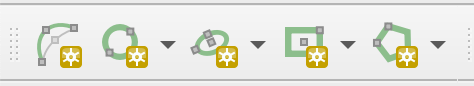
\includegraphics[keepaspectratio]{images/clipboard-3891180925.png}}
\end{center}

\begin{itemize}
\item
  \emph{циклическая строковая последовательность по радиусу}
  (\emph{Circular string by radius}) - отрисовка кривыми по двум точкам;
\item
  круг;

  \pandocbounded{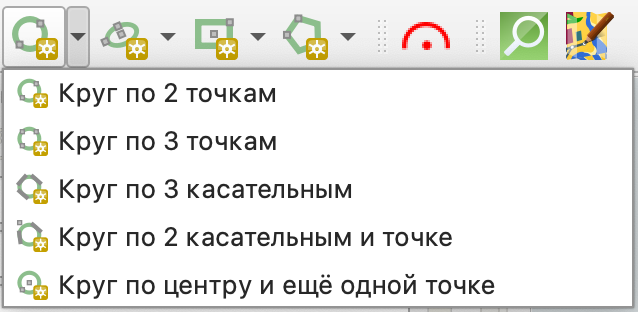
\includegraphics[keepaspectratio]{images/clipboard-1997811227.png}}
\item
  эллипс;
\end{itemize}

\begin{center}
\pandocbounded{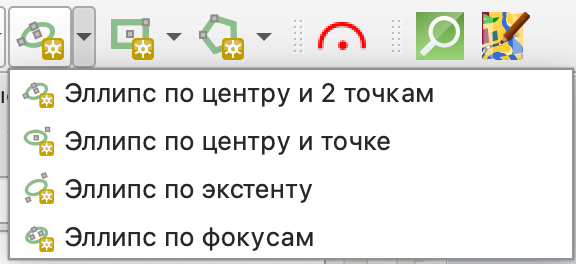
\includegraphics[keepaspectratio]{images/clipboard-472402114.png}}
\end{center}

\begin{itemize}
\tightlist
\item
  прямоугольник;
\end{itemize}

\begin{center}
\pandocbounded{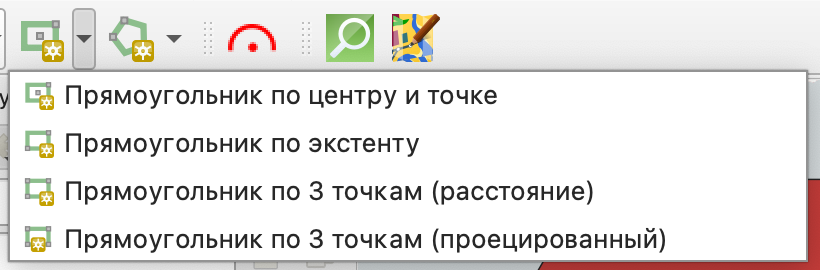
\includegraphics[keepaspectratio]{images/clipboard-1971131246.png}}
\end{center}

\begin{itemize}
\tightlist
\item
  создание правильного (выпуклого) многоугольника.
\end{itemize}

\begin{center}
\pandocbounded{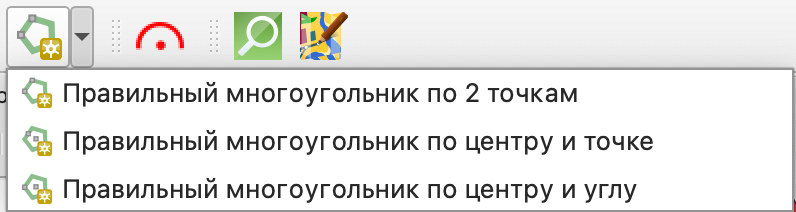
\includegraphics[keepaspectratio]{images/clipboard-3187458729.png}}
\end{center}

Для переноса объектов и их редактирования можно воспользоваться панелью
дополнительных инструментов оцифровки.

\begin{center}
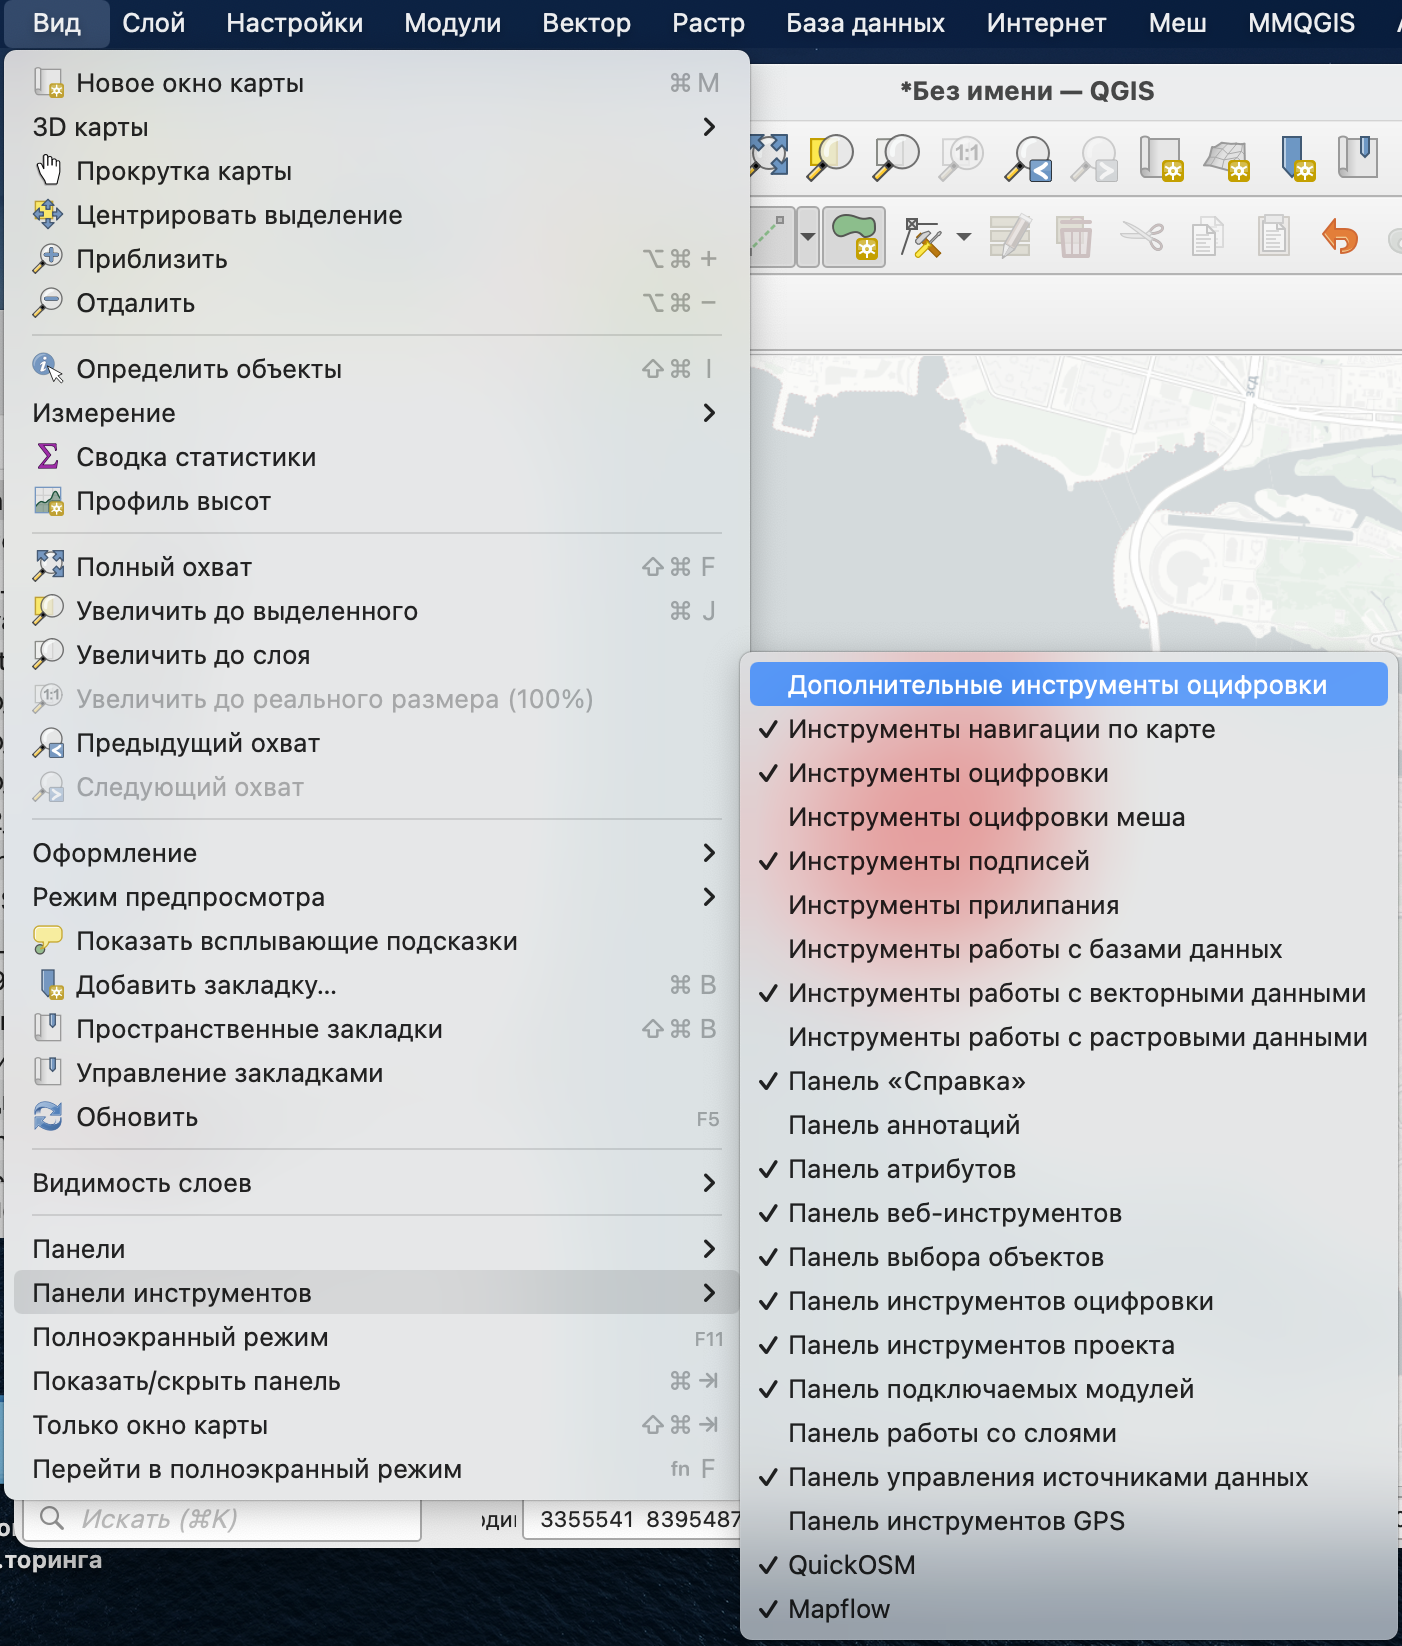
\includegraphics[width=7.98958in,height=\textheight,keepaspectratio]{images/clipboard-968594682.png}
\end{center}

Она будет добавлена на основную панель инструментов. С ее помощью вы
можете переносить объекты, поворачивать, вырезать отверстия в полигонах,
разрезать объекты и прочее.

\begin{center}
\pandocbounded{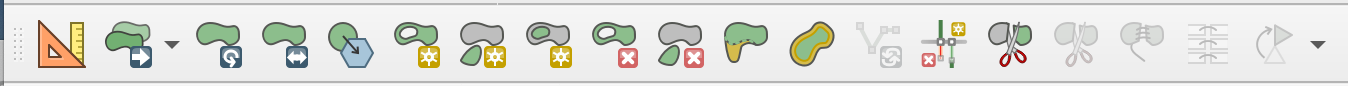
\includegraphics[keepaspectratio]{images/clipboard-2930058851.png}}
\end{center}

Если вы хотите отрисовывать объекты по их геометрическим параметрам:
углам между сотронами или сегментами линий, расстоянию, координатам
поворотных точек, то вы можете воспользоваться еще одной панелью
дополнительных инструментов оцифровки.

Ее можно включить или по клику на значок
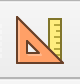
\includegraphics[width=0.34375in,height=0.35417in]{images/clipboard-2879122134.png},
или из строки меню.

\begin{center}
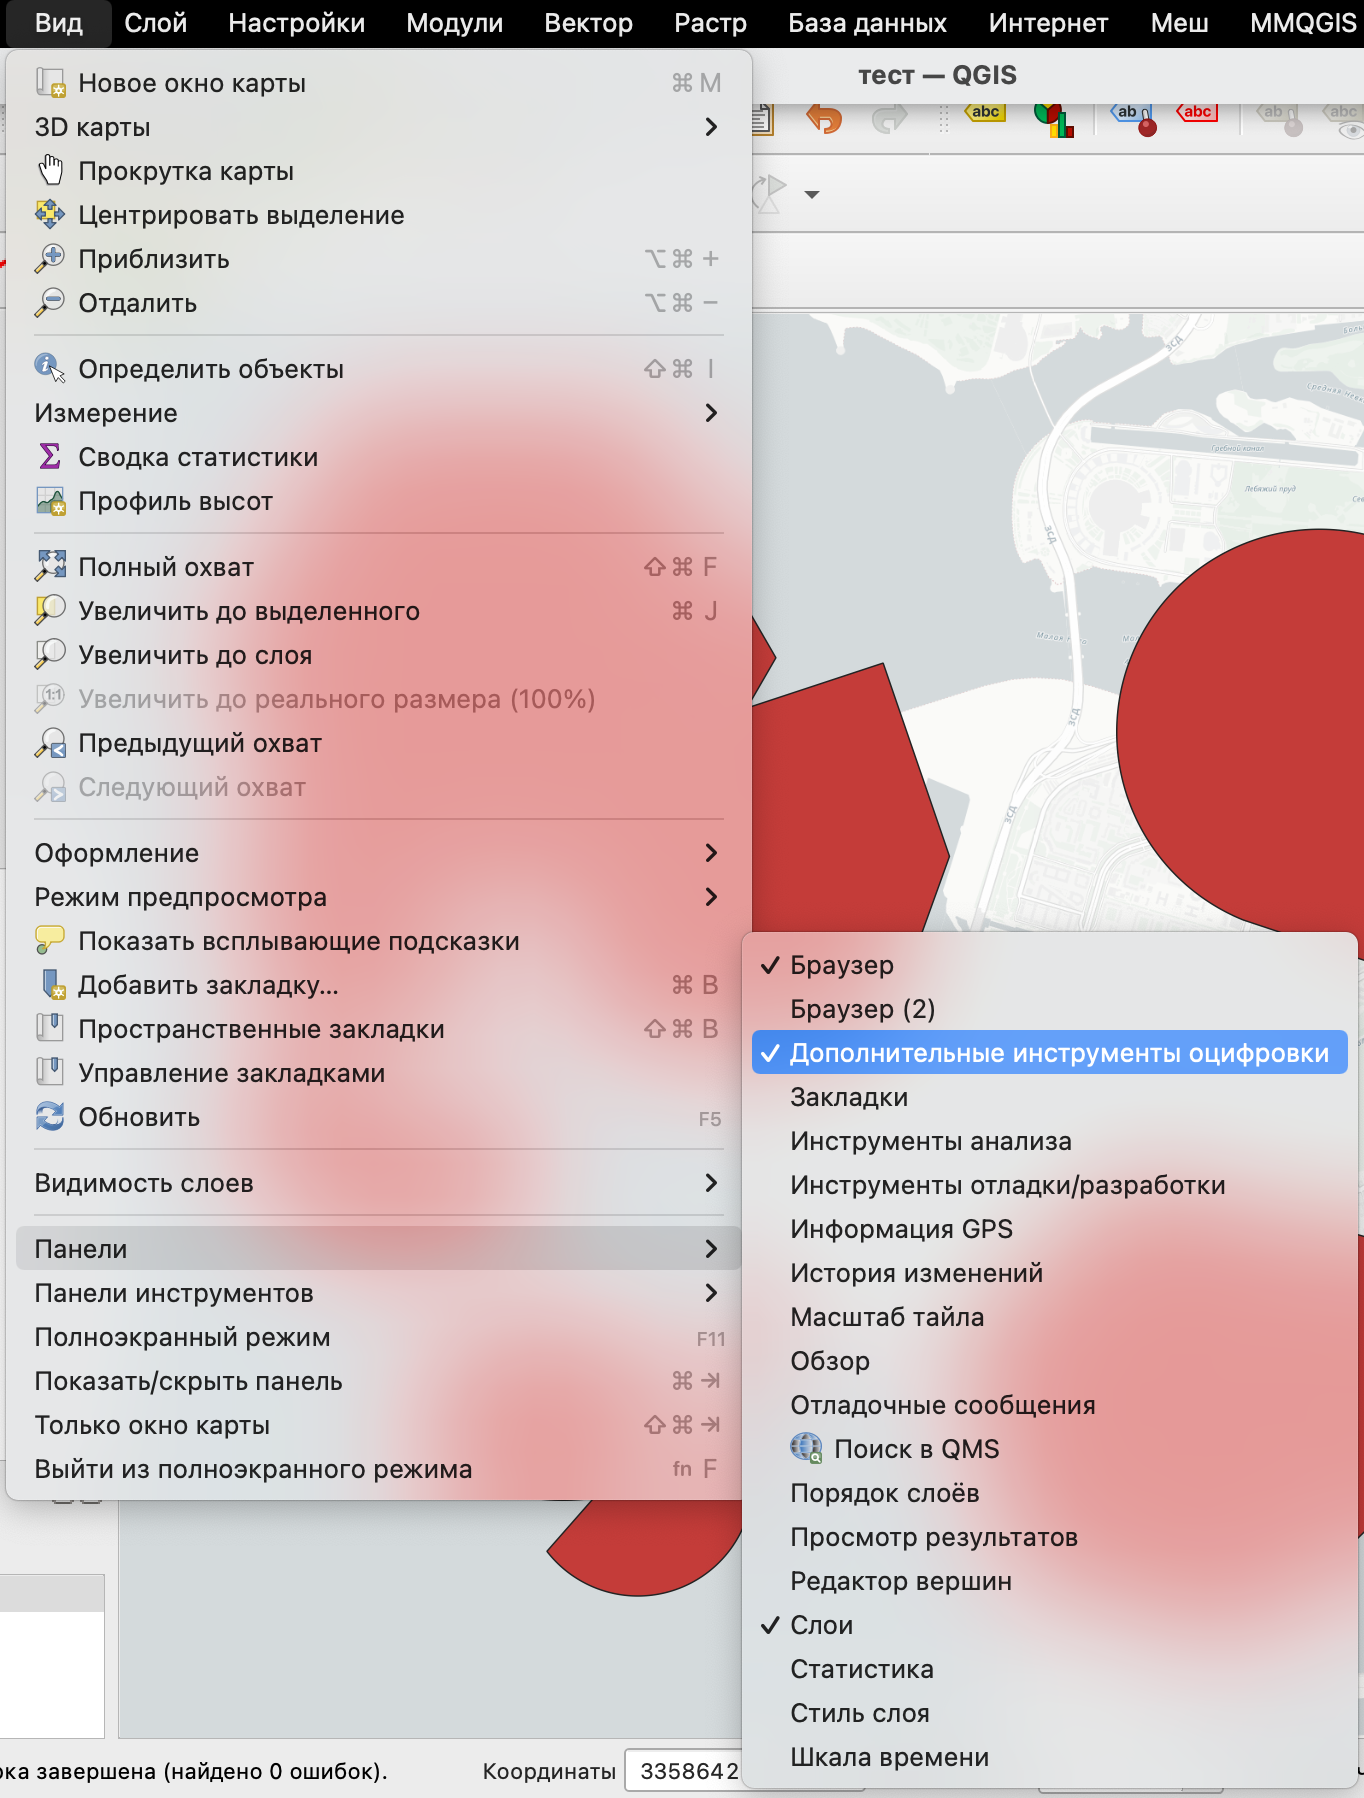
\includegraphics[width=7.11458in,height=\textheight,keepaspectratio]{images/clipboard-2835494369.png}
\end{center}

\begin{tcolorbox}[enhanced jigsaw, arc=.35mm, bottomrule=.15mm, bottomtitle=1mm, breakable, colback=white, colbacktitle=quarto-callout-caution-color!10!white, colframe=quarto-callout-caution-color-frame, coltitle=black, left=2mm, leftrule=.75mm, opacityback=0, opacitybacktitle=0.6, rightrule=.15mm, title=\textcolor{quarto-callout-caution-color}{\faFire}\hspace{0.5em}{Предупреждение}, titlerule=0mm, toprule=.15mm, toptitle=1mm]

Обратите внимание, что она открывается из пункта \emph{Панели} элемента
меню \emph{Вид}.

Наличие в меню одновременно пункта \emph{Панели} и \_Панели инструментов
связано с особенностями перевода: в оригинале это \emph{Panel} и
\emph{Toolbar} соответственно.

\end{tcolorbox}

\begin{center}
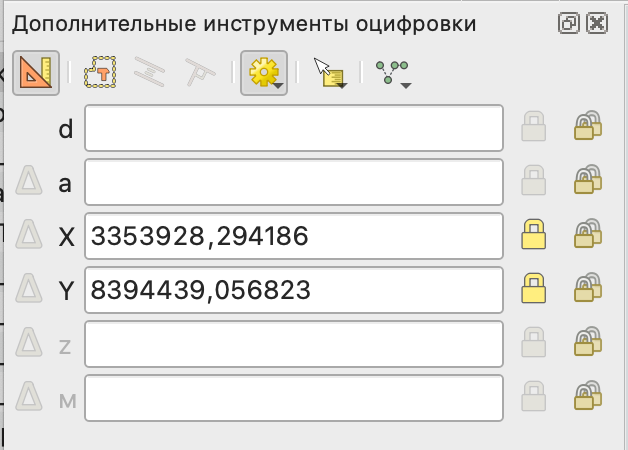
\includegraphics[width=5.8125in,height=\textheight,keepaspectratio]{images/clipboard-252496196.png}
\end{center}

\subsection{Привязка
объектов}\label{ux43fux440ux438ux432ux44fux437ux43aux430-ux43eux431ux44aux435ux43aux442ux43eux432}

В QGIS существует привязка объектов друг к другу, похожа по своему
принципу работы на объектную привязку в CAD системах.

Вы можете включить привязку объектов друг к другу по умолчанию в
настройках программы.

\begin{center}
\includegraphics[width=13.39583in,height=\textheight,keepaspectratio]{images/clipboard-3299530585.png}
\end{center}

Но здесь вы можете настроить только прилипание к одному типу элементов.
Для более контролируемой привязки объектов лучше воспользоваться
\emph{Инструментами прилипания}, которые можно добавить на панель
инструментов из строки меню.

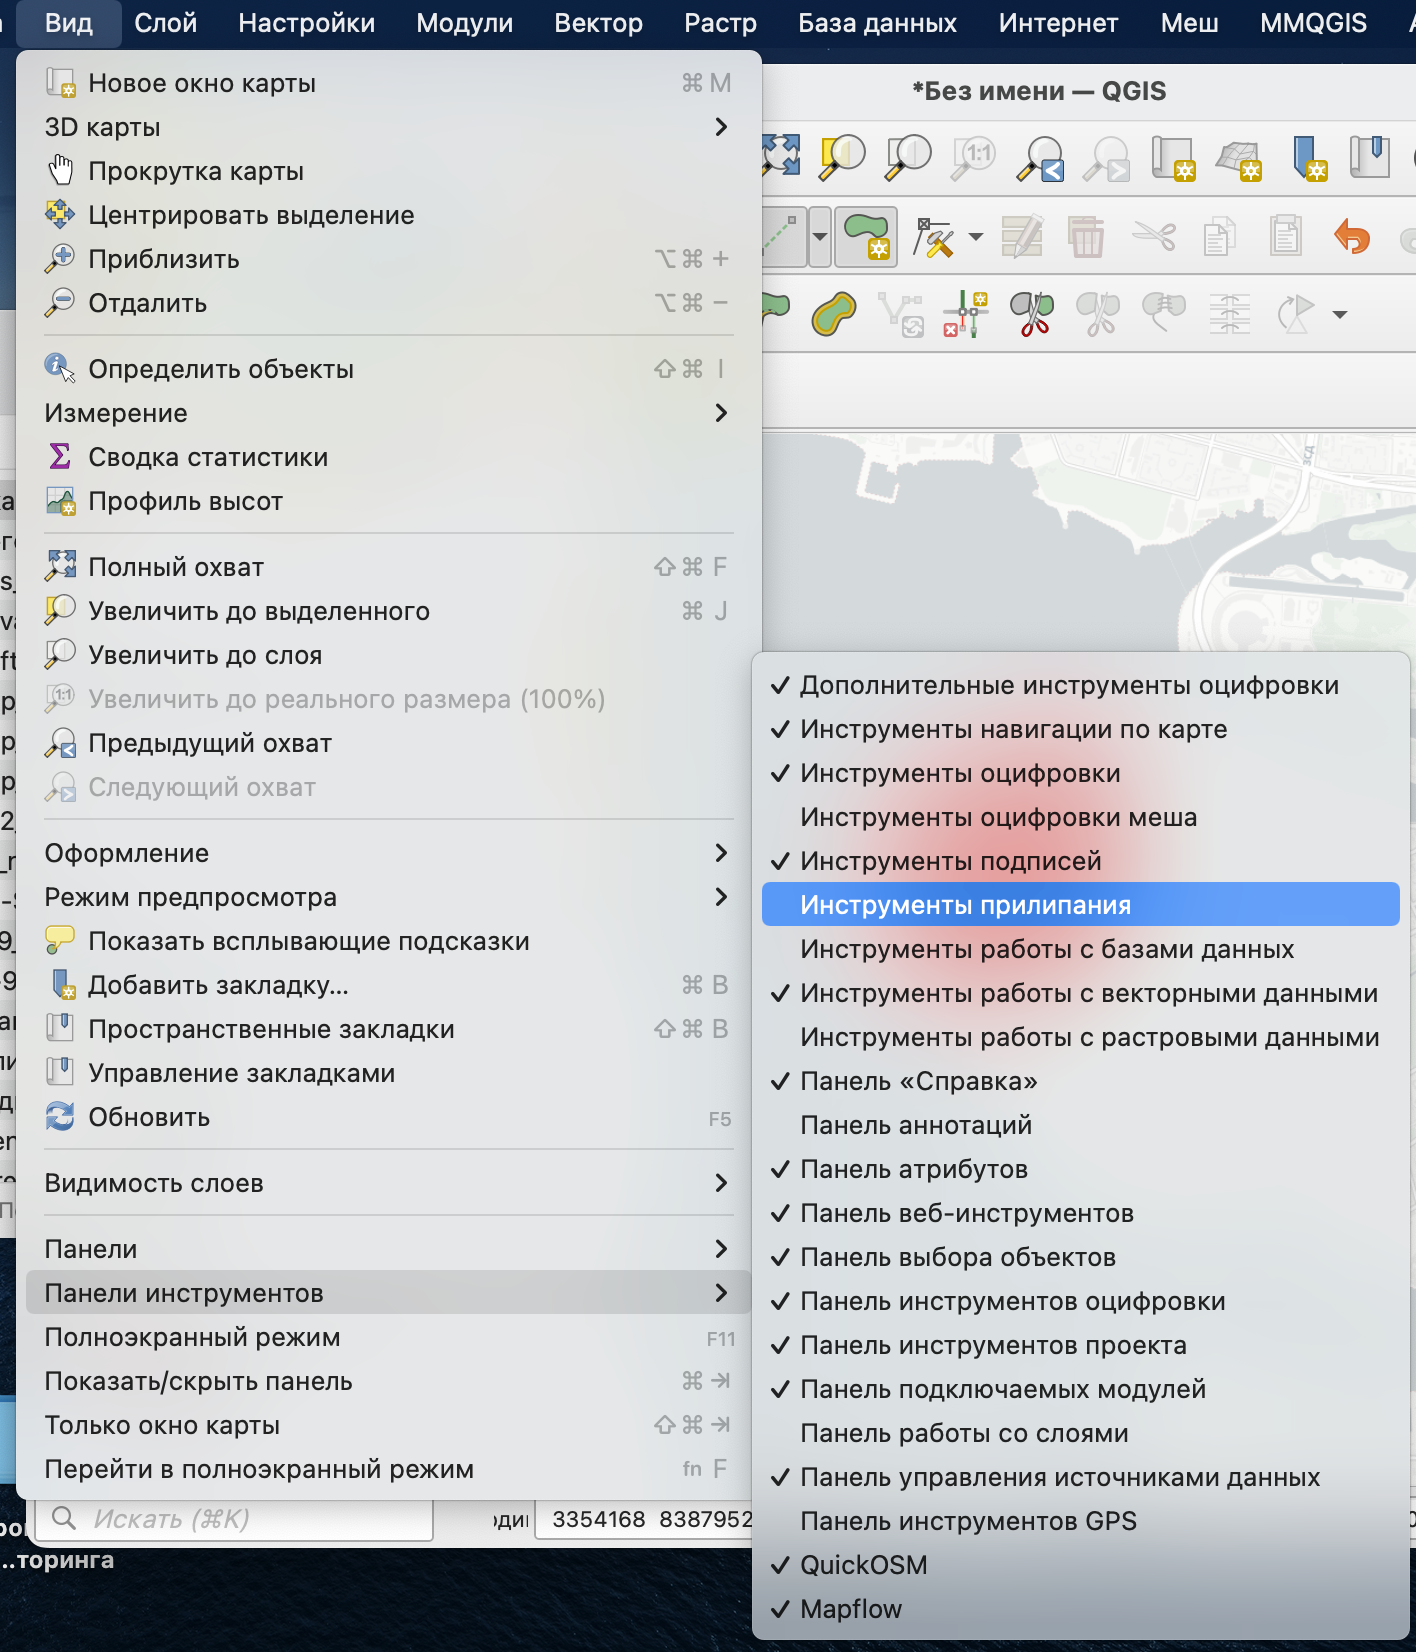
\includegraphics[width=8.03125in,height=\textheight,keepaspectratio]{images/clipboard-2306646983.png}

Эта панель активируется по клику на символ магнита.

\begin{center}
\pandocbounded{
\includegraphics[keepaspectratio]{images/clipboard-2945452430.png}}
\end{center}

Основные инструменты панели (слева направо):

\begin{itemize}
\item
  разрешить прилипание;
\item
  выбор слоев, для которых будет доступно прилипание: все слои -
  прилипание будет осуществляться с учетом объектов всех слоев, которые
  есть в проекте (даже невидимых в данный момент), активный слой -
  прилипание будет осуществляться только для объектов текущего слоя.
\item
  тип объектов, к которым осуществляется прилипание (может быть выбрано
  сразу несколько вариантов):

  \begin{itemize}
  \item
    к вершинам - прилипание только к узловым точкам;
  \item
    к линиям - прилипание к любой точке линии;
  \item
    к поверхности - прилипание к любой точке внутри полигона;
  \item
    к центроиду - прилипание к геометрическому центру полигона;
  \item
    середина отрезка - прилипание только к середине линии;
  \item
    конечные точки линии - прилипание только к начальной или конечной
    точке линии.
  \end{itemize}
\end{itemize}

\begin{center}
\pandocbounded{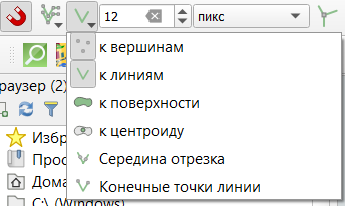
\includegraphics[keepaspectratio]{images/clipboard-4188854556.png}}
\end{center}

\begin{itemize}
\item
  порог прилипания - то есть, в какой области вокруг курсора будет
  искаться объект для прилипания;
\item
  топологическое редактирование позволяет сохранять общие границы между
  объектами. Если эта опция включена, то программа будет автоматически
  перестраивать общую границу для двух объектов (если таковая граница
  есть);
\item
  допустимы ли наложения между объектами;
\end{itemize}

\begin{center}
\pandocbounded{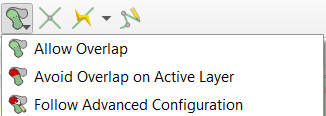
\includegraphics[keepaspectratio]{images/clipboard-3799602480.png}}
\end{center}

\begin{itemize}
\item
  разрешать прилипание к пересечениям - прилипание будет осуществляться
  к пересечениям двух объектов, даже если там нет вершины;
\item
  трассирование (tracing) - позволяет ускорить привязку к линейным
  объектам, при включении этой опции вам не нужно будет прощелкивать по
  всей линии, достаточно будет нескольких точек (если установить
  значение отступа offset, то можно построить линию, параллельную
  существующей);
\item
  самоприлипание - позволяет осуществлять привязку отрисовываемого
  объекта к самому себе.
\end{itemize}

\subsection{Редактирование формы
объектов}\label{ux440ux435ux434ux430ux43aux442ux438ux440ux43eux432ux430ux43dux438ux435-ux444ux43eux440ux43cux44b-ux43eux431ux44aux435ux43aux442ux43eux432}

Основной инструмент редактирования формы - \emph{Инструмент
редактирования вершин}
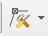
\includegraphics[width=0.46875in,height=0.34375in]{images/clipboard-4065537032.png}
предназначен для редактирования линий и полигонов.

Для того, чтобы его активировать необходимо, чтобы ваш слой был
редактируемым и активен инструмент рисования.

Этот инструмент может работать как только в текущем активном слое, так и
для всех слоев одновременно (что может быть удобно, если у вас несколько
слоев для редактирования и вы не хотите постоянно переключаться между
ними.

После активации инструмента у вас в правой части окна появится небольшая
панель редактированимя вершин, в которой вам предлагается возможность
просмотра каталога вершин объектов.

\begin{center}
\pandocbounded{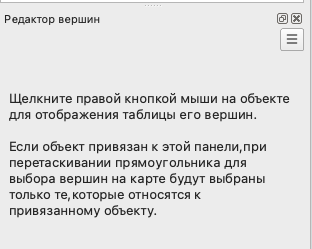
\includegraphics[keepaspectratio]{images/clipboard-1852560836.png}}
\end{center}

В панели редактора отображаются координаты точек в системе координат
слоя.

\begin{center}
\pandocbounded{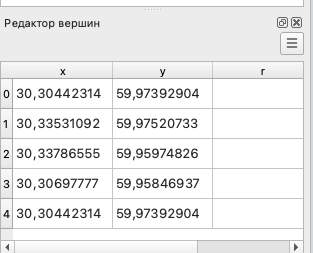
\includegraphics[keepaspectratio]{images/clipboard-2659992431.png}}
\end{center}

При простом наведении на объект вы увидите, что его контур будет
подсвечиваться и узлы отображаться более крупно.

\subsection{Редактирование структуры таблицы
атрибутов}\label{ux440ux435ux434ux430ux43aux442ux438ux440ux43eux432ux430ux43dux438ux435-ux441ux442ux440ux443ux43aux442ux443ux440ux44b-ux442ux430ux431ux43bux438ux446ux44b-ux430ux442ux440ux438ux431ux443ux442ux43eux432}

Атрибуты - это непространственные характеристики объектов, которые
отображаются в табличном виде, где одна строка таблицы - это один
объект, а каждый столбец - это характеристика объекта.

Открыть таблицу атрибутов можно из контекстного меню слоя.

\begin{center}
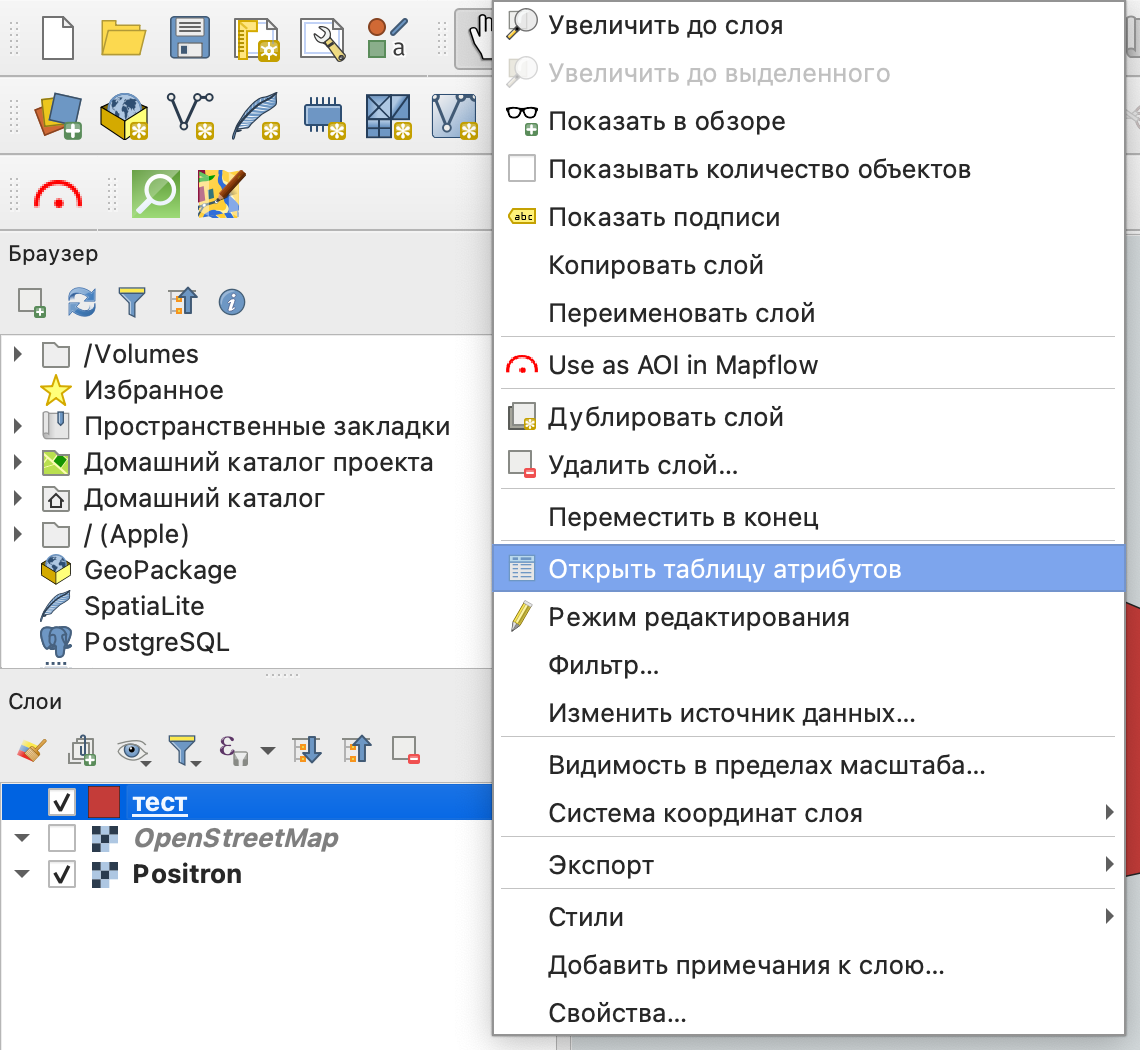
\includegraphics[width=9.05208in,height=\textheight,keepaspectratio]{images/clipboard-1516570935.png}
\end{center}

Когда вы выделяете объект на карте, он выделяется в таблице атрибутов, и
наоборот.

\begin{center}
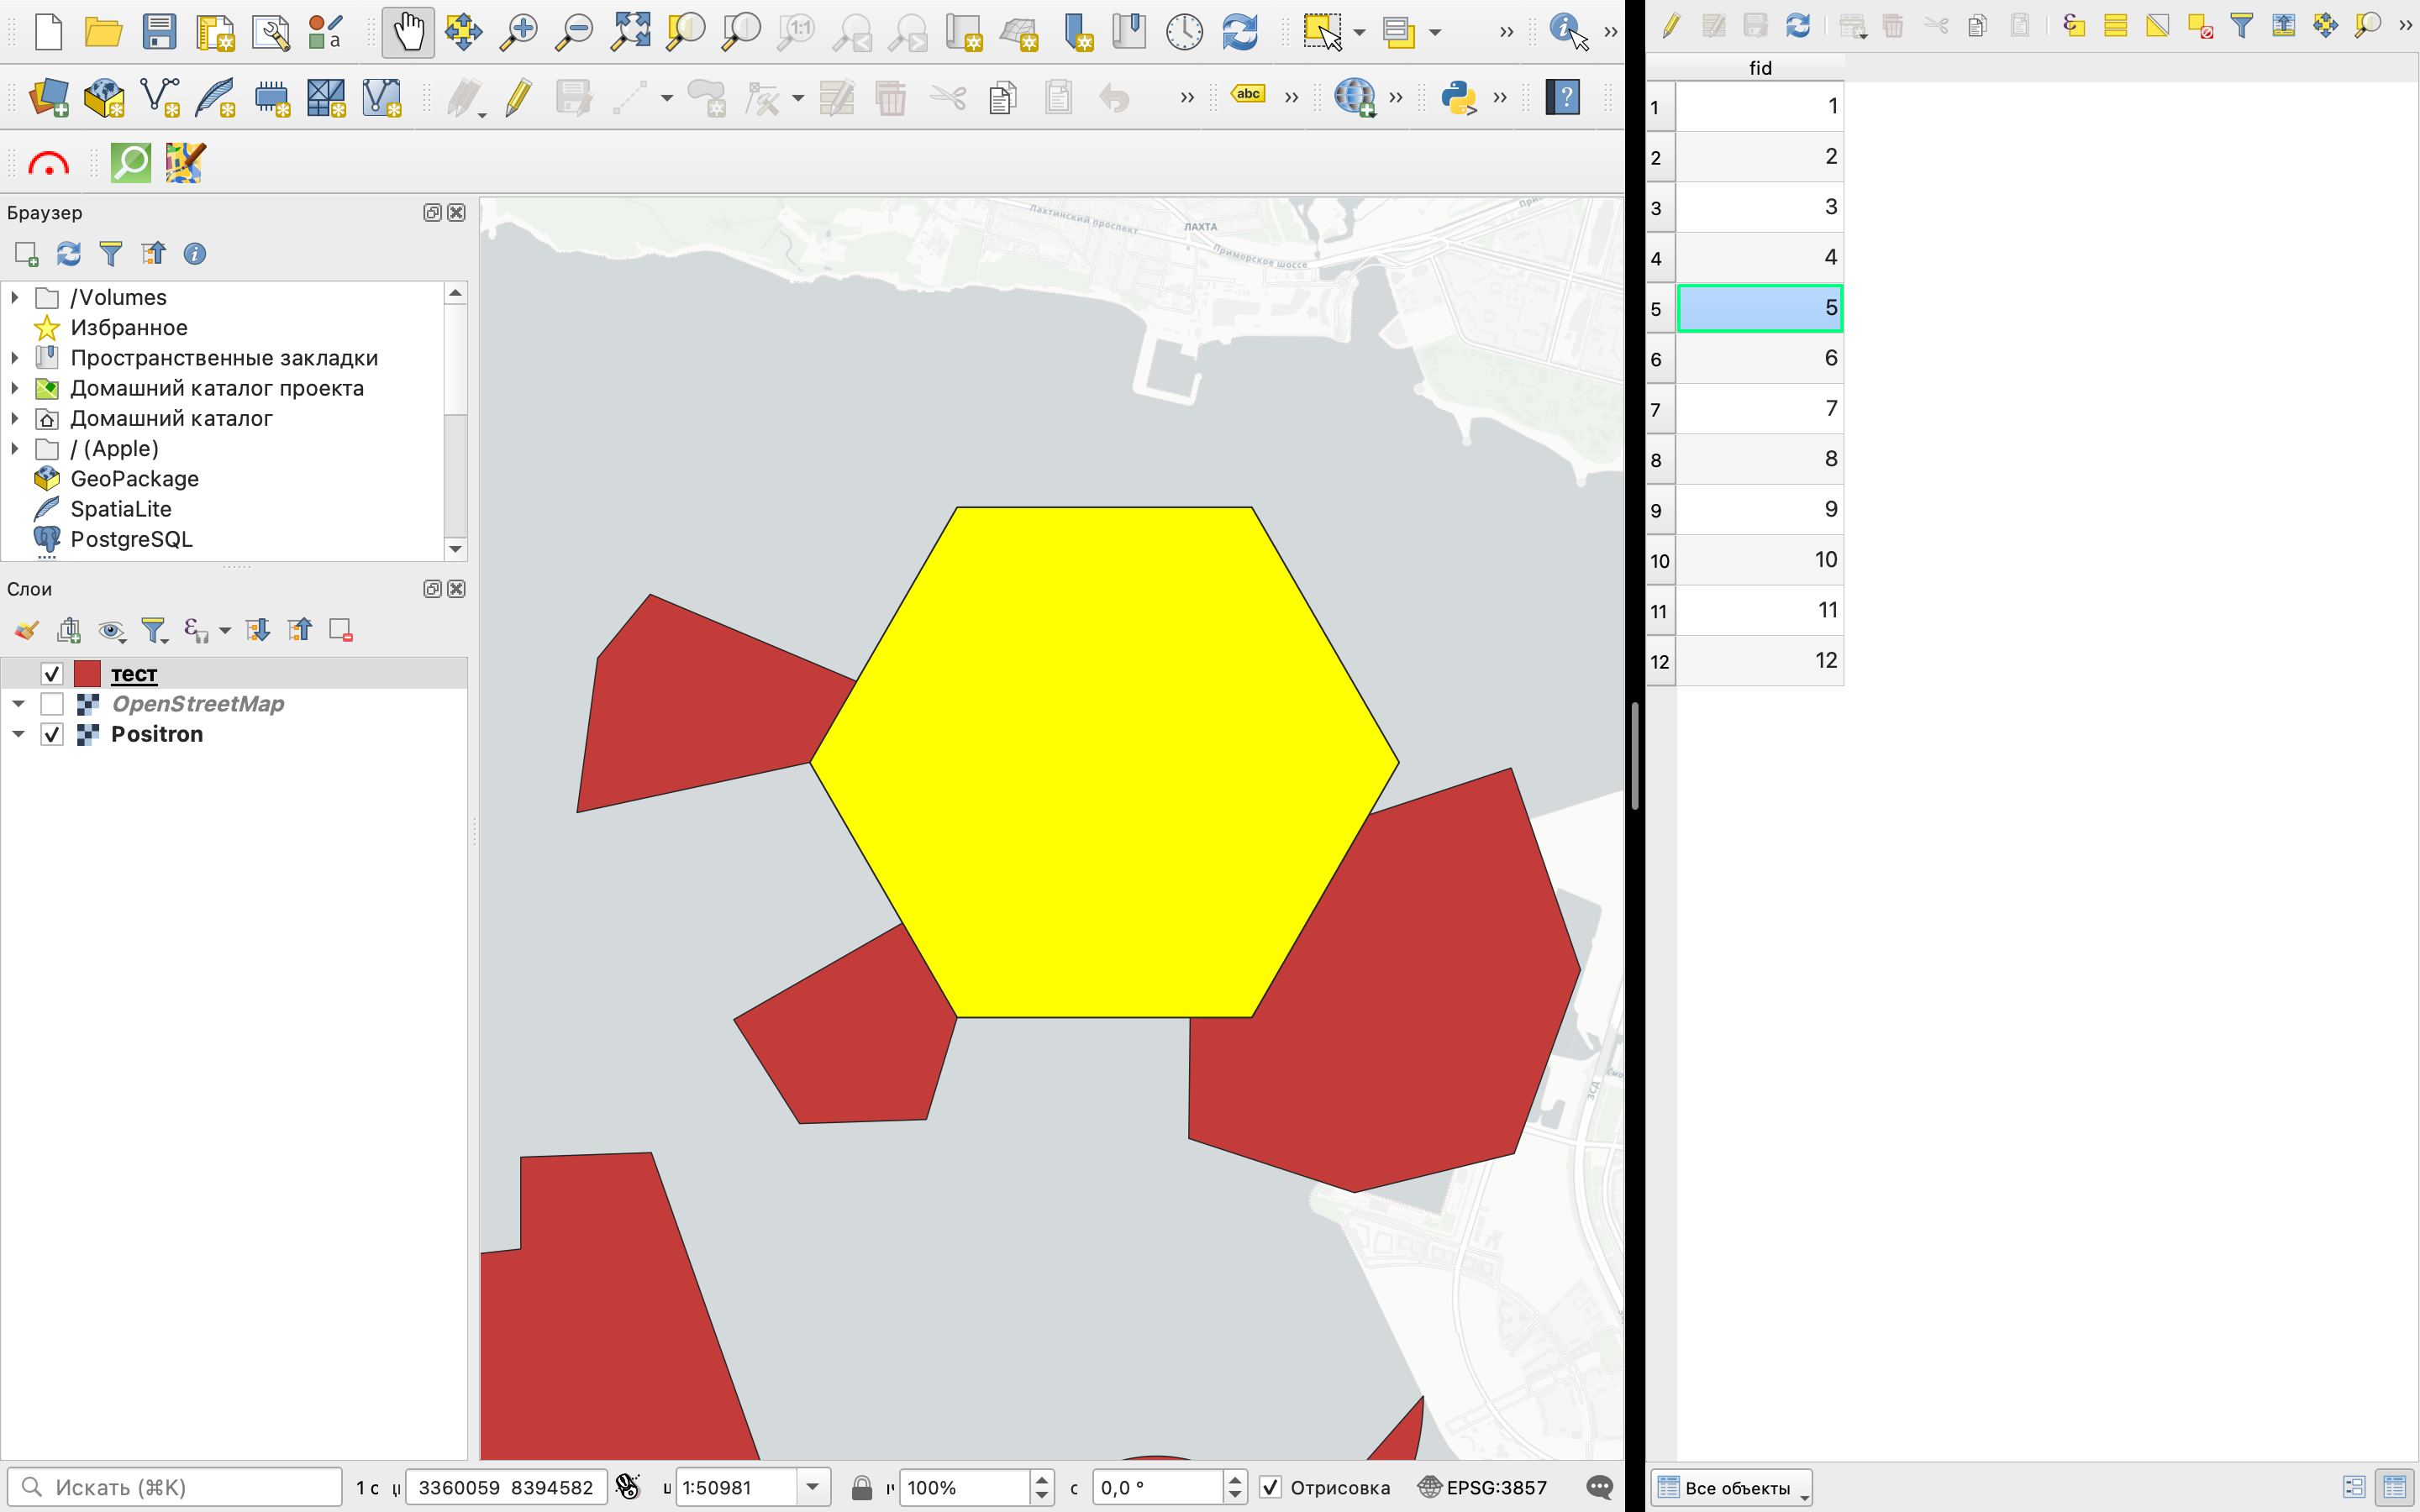
\includegraphics[width=15in,height=\textheight,keepaspectratio]{images/clipboard-1452138254.png}
\end{center}

У таблицы атрибутов есть своя собственная панель инструментов.

\begin{center}
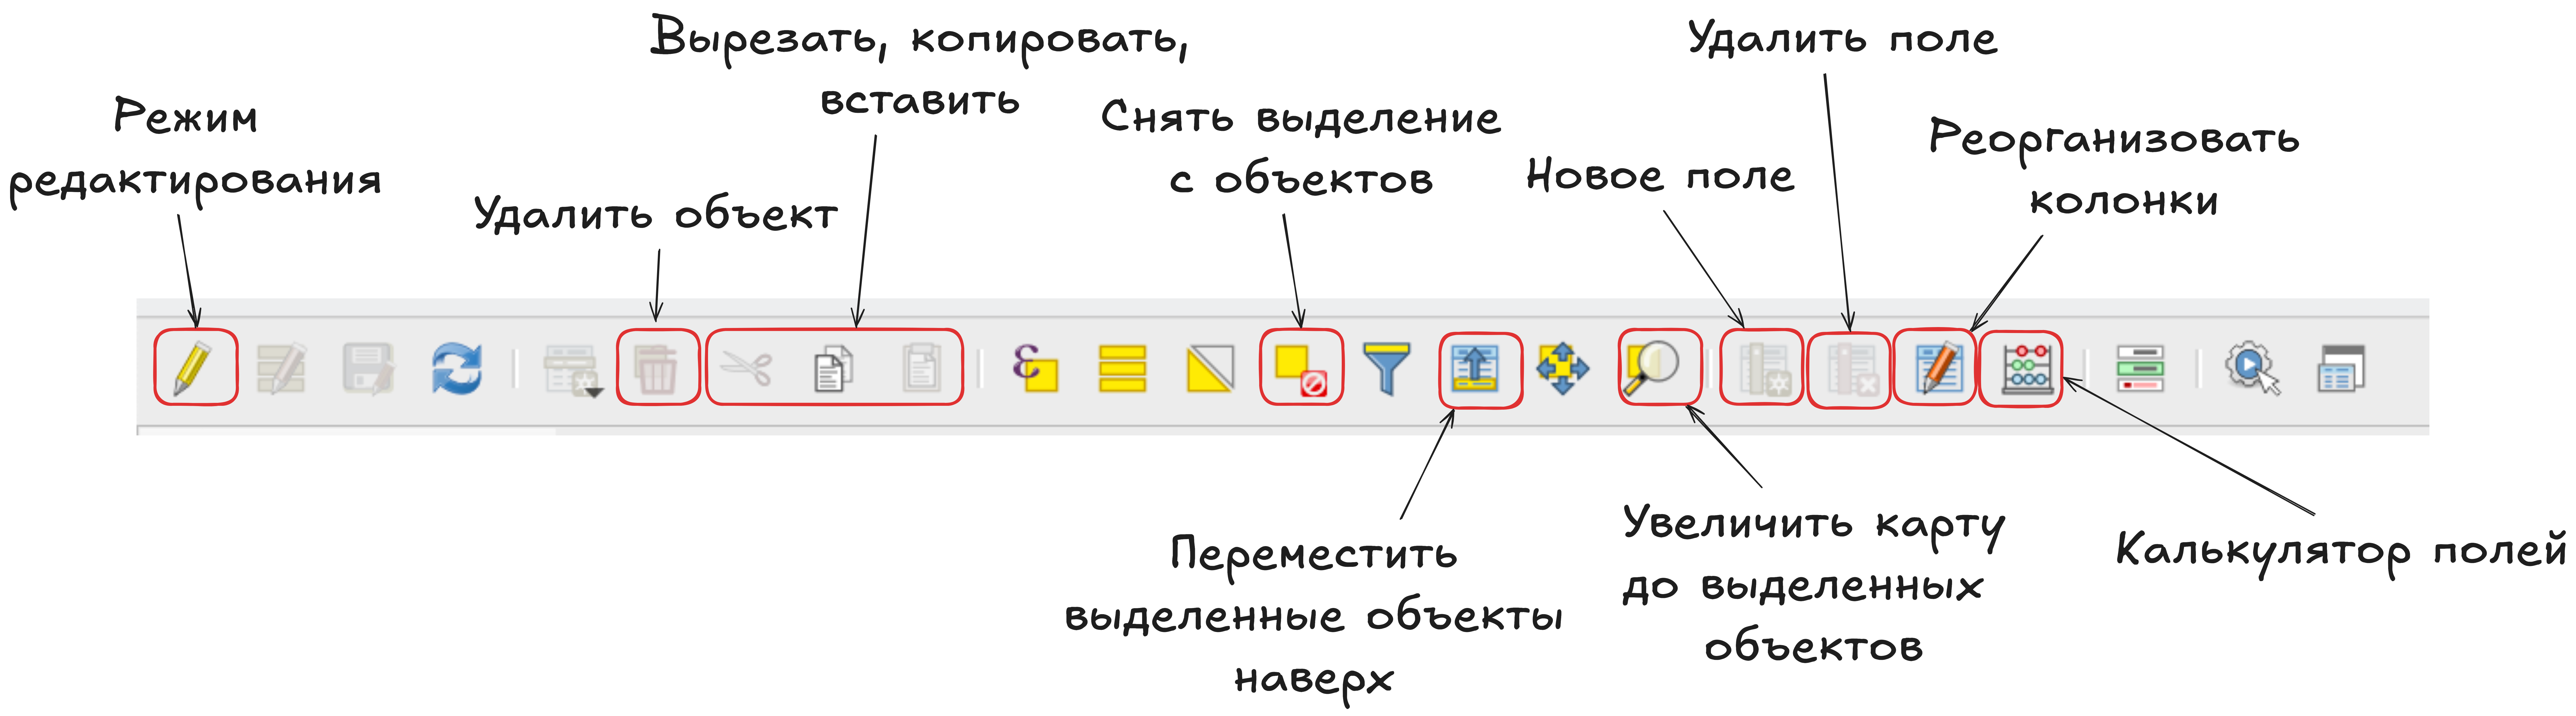
\includegraphics[width=22.47917in,height=\textheight,keepaspectratio]{images/clipboard-1045039255.png}
\end{center}

При добавлении нового поля необходимо указать его имя (оно должно быть
уникальным в рамках таблицы атрибутов) и тип данных, которые будут
содержаться в этом поле.

\begin{center}
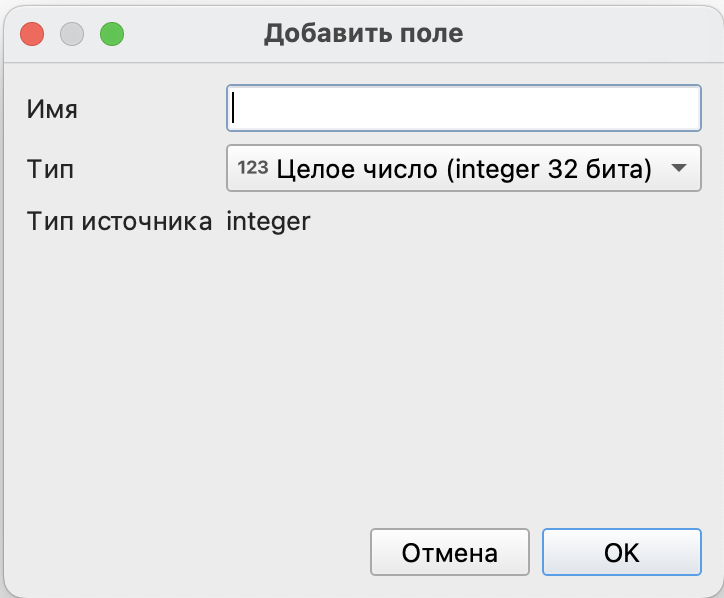
\includegraphics[width=6.30208in,height=\textheight,keepaspectratio]{images/clipboard-996559067.png}
\end{center}

При удалении полей, если вы хотите удалить несколько из них, вы можете
выделить в списке их все, просто кликнув на названия.

Реорганизация полей значит изменение их порядка в таблице, для нее вы
можете просто перетащить названия полей в списке, установив тот порядок,
который хотите. В списке ваши поля будут перечислены сверху вниз, что
соответствует их порядку в таблице слева-направо.

Калькулятор полей необходим для создания вычисляемых полей или
обновления значений в уже существующих полях. Мы будем активно работать
с калькулятором полей в более поздних разделах.

\end{document}
